\documentclass[semifinal]{cpecmu}

%% This is a sample document demonstrating how to use the CPECMU
%% project template. If you are having trouble, see "cpecmu.pdf" for
%% documentation.

\projectNo{69}
\acadyear{2020}

\titleTH{ระบบการจัดการ Nursery}
\titleEN{Nursery Management System}

\author{นายพงศ์ภัค เกษมศรี ณ อยุธยา}{Pongpuk Kasemsee Na Ayutaya}{600610754}
\author{นายศุภกร หอมน่าน}{Suphakorn Homnan}{600610782}

\cpeadvisor{chinawat}
\cpecommittee{paskorn}
\committee{รศ.ดร.\,นิพนธ์ ธีรอำพน}{Assoc.\,Prof.\,Nipon Theera-Umpon, Ph.D.}

%% Some possible packages to include:
\usepackage[final]{graphicx} % for including graphics

%% Add bookmarks and hyperlinks in the document.
\usepackage[colorlinks=true,allcolors=Blue4,citecolor=red,linktoc=all]{hyperref}

%% Set up commenting
\iffinal
  \usepackage[disabled]{authcomments}
\else
  \usepackage{authcomments}
\fi
\newcommenter{CI}{0.0,0.5625,0.0}  % green

%% Needed just by this example, but maybe not by most reports
\usepackage{afterpage} % for outputting
\usepackage{pdflscape} % for landscape figures and tables. 

%% Some other useful packages. Look these up to find out how to use
%% them.
% \usepackage{natbib}    % for author-year citation styles
% \usepackage{txfonts}
% \usepackage{appendix}  % for appendices on a per-chapter basis
% \usepackage{xtab}      % for tables that go over multiple pages
% \usepackage{subfigure} % for subfigures within a figure
% \usepackage{pstricks,pdftricks} % for access to special PostScript and PDF commands
% \usepackage{nomencl}   % if you have a list of abbreviations

%% if you're having problems with overfull boxes, you may need to increase
%% the tolerance to 9999
% \tolerance=9999

\bibliographystyle{plain}
% \bibliographystyle{IEEEbib}

% \renewcommand{\topfraction}{0.85}
% \renewcommand{\textfraction}{0.1}
% \renewcommand{\floatpagefraction}{0.75}

%% Example for glossary entry
%% Need to use glossary option
%% See glossaries package for complete documentation.
\ifglossary
  \newglossaryentry{lorem ipsum}{
    name=lorem ipsum,
    description={derived from Latin dolorem ipsum, translated as ``pain itself''}
  }
\fi

%% Uncomment this command to preview only specified LaTeX file(s)
%% imported with \include command below.
%% Any other file imported via \include but not specified here will not
%% be previewed.
%% Useful if your report is large, as you might not want to build
%% the entire file when editing a certain part of your report.
% \includeonly{chapters/intro,chapters/background}

\begin{document}
\maketitle
\makesignature

\ifproject
\begin{abstractTH}
    การบริหารจัดการเนอสเซอรี่จําเป็นต้องจัดเก็บข้อมูลเพื่อใช้ในการตรวจสอบความพร้อมของเด็กในแต่ละวัน อาทิ สถิติการมา–ขาด อุปกรณ์ส่วนตัว และข้อมูลสุขภาพ รวมไปถึงข้อมูลยามฉุกเฉิน อาทิ หมายเลขติดต่อผู้ปกครอง โรงพยาบาลฉุกเฉิน และข้อมูลส่วนบุคคล ในปัจจุบัน การเก็บข้อมูลดังกล่าวยังคง ใช้วิธีกรอกลงบนเอกสาร ซึ่งเกิดความผิดพลาดได้ง่าย ใช้เวลานาน และสิ้นเปลืองทรัพยากรกระดาษโดยใช่เหตุ นอกจากนี้ หลังจากเก็บข้อมูลลงกระดาษแล้ว ทางเนอสเซอรี่เองยังจําเป็นต้องกรอกข้อมูลลงในคอมพิวเตอร์อีกครั้งหนึ่ง 
    เพื่อป้องกันการสูญหายและอํานวยความสะดวกในการค้นหาข้อมูล โครงงานนี้มุ่งที่จะแก้ไขปัญหาและอุปสรรคดังกล่าว โดยการสร้างโปรแกรมประยุกต์บนเว็บ (web application) สําหรับจัดการข้อมูลภายเนอสเซอรี่ เพื่อเก็บข้อมูลโดยตรง ทําให้ลดความยุ่งยากในการจัดเก็บข้อมูล ลดความผิดพลาดในการกรอกข้อมูล และยังสามารถนําข้อมูลที่มีอยู่ไปวิเคราะห์และแสดงผลเพื่อให้เห็นข้อมูลภาพรวมของเด็กได้ชัดเจนยิ่งขึ้น นอกจากนี้การใช้ระบบจัดการเนอสเซอรี่ยังช่วยลดการสูญหายของข้อมูลระหว่างการจัดเก็บ (เช่น การสูญหายของเอกสารที่มักพบในการเก็บข้อมูลในแบบเก่า และการเกิดความเสียหายของเอกสาร)  ระบบจัดการเนอสเซอรี่นี้จะช่วยให้การบริหารจัดการเป็นไปอย่างคล่องตัวและเบ็ดเสร็จ ตั้งแต่กระบวนการรับเด็กแรกเข้า การเลื่อนชั้น จนกระทั่งถึงเวลาที่เด็กพร้อมจะเข้าเรียนในระดับอนุบาล


\end{abstractTH}

\begin{abstract}
    Nursery Management needs to store information to be used to observe the Readiness of each child each day such as The Attendance Statistics, The list of personal equipment and Health information, Including emergency information such as parent's emergency contact numbers and Preferred hospital. Nowadays, The collection of such information is still done by pen and paper.  This causes unnecessary paper consumption.  Moreover, When mistakes happen they take a long time to be corrected. Also to prevent loss and to facilitate convenient lookups The Nursery needs to reenter all the information on the computer anyway.
    The purpose of this project is to eliminate the unnecessary workflow by creating a Web Application for managing data within the Nursery. Although outside the scope of this project, The collected information can be used afterward for analyses and display to give a clearer perspective of the child. Using a Nursery Management System can also reduce data loss during storage (such as Document losses and Damages often found in old-fashioned archives).  This Web Application aims to be a one-stop service in managing the Nursery from the moment a child enters the Nursery to departure for Kindergarten.
\end{abstract}

\iffalse
\begin{dedication}
This document is dedicated to all Chiang Mai University students.

Dedication page is optional.
\end{dedication}
\fi % \iffalse

\begin{acknowledgments}
โครงงานนี้สำเร็จลุล่วงได้ด้วยความกรุณาจากอาจารย์ชินวัตร อิศราดิสัยกุล อาจารย์ที่ปรึกษาโครงงานที่ได้ให้คำแนะนำและข้อเสนอแนะ แนวคิด ตลอดจนการค่อยเฝ้าติดตามและแก้ไขข้อบกพร่องต่างๆ ตลอดจนโครงงานเล่มนี้เสร็จสมบูรณ์
ผู้ศึกษาจึงขอกราบขอบพระคุณเป็นอย่างยิ่ง
ขอกราบขอบพระคุณคณะกรรมการสอบโครงงาน อาจารย์นวดนย์ คุณเลิศกิจ และ อาจารย์พฤษภ์ บุญมา ที่ค่อยให้คำแนะนำและข้อเสนอแนะต่างๆ ผู้ศึกษาจึงขอกราบขอบพระคุณเป็นอย่างยิ่ง
ขอบคุณเพื่อนๆที่ค่อยช่วยเหลือและให้คำแนะนำต่างๆ เกี่ยวกับโครงงานนี้
สุดท้ายนี้ขอขอบคูณทางพีคอะบู เนอร์สเซอรี่ ที่ได้ให้ความร่วมมือในการลองใช้งานระบบจัดการ nursery จนทำให้โครงงานสำเร็จลุล่วงไปได้ด้วยดี

\acksign{2021}{4}{6}
\end{acknowledgments}%
\fi % \ifproject

\contentspage

\ifproject
\figurelistpage

\fi % \ifproject

% \abbrlist % this page is optional

% \symlist % this page is optional

% \preface % this section is optional


\pagestyle{empty}\cleardoublepage
\normalspacing \setcounter{page}{1} \pagenumbering{arabic} \pagestyle{cpecmu}

\chapter{\ifcpe บทนำ\else Introduction\fi}

\section{\ifcpe ที่มาของโครงงาน\else Project rationale\fi}

ในปัจจุบันเทคโนโลยีได้เข้ามามีบทบาทในชีวิตประจําวันในทุกๆ ด้าน โดยในแต่ละด้านก็มีการนําเทคโนโลยีมาใช้ทดแทนแรงงานคน  เพื่ออํานวยความสะดวกในการทํางานของเจ้าหน้าที่ฝ่ายต่างๆ  ยกตัวอย่างเช่น แพลตฟอร์มลงทะเบียนสอบ GAT/PAT ออนไลน์ application ที่ใช้จัดการกับระบบต่างๆภายในบริษัทหรือองค์กร สำนักงานต่างๆ ระบบจัดการภายในโรงพยาบาล ระบบจองคิวรับคิวภายในร้านอาหาร เป็นต้น

แต่ว่าในภาคส่วนของทาง nursery ยังไม่ค่อยพบเห็นแพลตฟอร์มหรือระบบจัดการภายในแบบออนไลน์เท่าใดนัก
เนื่องจาก nursery เป็นองค์กรที่มีขนาดเล็ก ไม่ได้มีระบบการบริหารจัดการจากส่วนกลาง จึงทำให้ผู้พัฒนาหลายๆ กลุ่มมองไม่เห็นความสำคัญของปัญหาที่เกี่ยวกับการจัดการ nursery ได้แก่ การจัดเก็บข้อมูลต่างๆ รายวัน ซึ่งในปัจจุบันยังทำลงบนกระดาษอยู่ ส่งผลให้เกิดปัญหาความล่าช้าในกระบวนการรวบรวมและจัดเก็บข้อมูล
นอกจากนี้ การแก้ไขหรือเข้าถึงข้อมูลต่างๆ เช่น การตรวจสอบและแก้ไขประวัติเด็ก ย่อมเกิดความล่าช้า เนื่องจากจำเป็นต้องดำเนินการผ่านเจ้าหน้าที่ของ nursery ยิ่งไปกว่านั้น ยังมีเรื่องของความเสี่ยงในการที่เอกสารที่จัดเก็บไว้จะสูญหายหรือสูญเสียอีกด้วย

จากเหตุผลที่กล่าวมาข้างต้น ทางผู้จัดทําจึงได้นำแนวคิดนี้มาสร้างเป็น web application 
สําหรับจัดการภายในเนอสเซอรี่ เพื่อให้ครูและเจ้าหน้าที่ใน nursery สามารถตรวจสอบและแสดงข้อมูลของเด็กได้โดยง่ายและสะดวกรวดเร็วขึ้น และเพื่อลดการสูญหายของข้อมูลระหว่างการจัดส่งหรือจัดเก็บ ที่อาจเกิดขึ้นได้จากการใช้กระดาษ
นอกเหนือจากการจัดเก็บข้อมูลส่วนบุคคลของเด็กแต่ละคนแล้ว ระบบจัดการภายใน nursery ที่ผู้จัดทำได้วางแผนพัฒนานั้น จะสามารถรองรับการจัดการกิจวัตรประจำวันต่างๆ ภายใน nursery ได้แก่ การเช็คชื่อ เช็คของใช้ เช็คสุขภาพ
ซึ่งสามารถทำได้แบบ real-time ผ่านระบบออนไลน์
ในท้ายที่สุด ระบบจัดการ nursery ที่จะพัฒนานั้น จะมีการจัดการคลังสินค้าของทาง nursery และ ระบบ payment สำหรับจัดการกับประวัติการจ่ายเงินค่าเล่าเรียนใน nursery



\section{\ifcpe วัตถุประสงค์ของโครงงาน\else Objectives\fi}
\begin{enumerate}
    \item เพื่อลดความยุ่งยากในการตรวจสอบข้อมูลของเด็กแต่ละคน ซึ่งในการตรวจสอบข้อมูลเด็กแต่ละคนใน แบบเก่า (เอกสารและexcel) กว่าที่เราจะได้ข้อมูลมาต้องผ่านกระบวนการต่างๆ มากมาย อาทิเช่น การนั่งค้นหากองเอกสารเพื่อหาเอกสารที่บันทึกข้อมูลของเด็กที่ต้องการ หรือการมานั่งค้นหาข้อมูลใน excel ซึ่งอาจจะเสียเวลาได้หากมีการบันทึกไฟล์ไว้หลายๆไฟล์ ทาง web application ของเราจะเข้ามาจัดการกับปัญหานี้ โดยทําให้ขั้นตอนนี้เหล่านี้สามารถเข้าถึงข้อมูลได้รวดเร็วและสะดวกยิ่งขึ้น 

    \item สามารถตรวจสอบการเข้าเรียน ตรวจเช็คอุปกรณ์ ตรวจเช็คสุขภาพของเด็กในแต่ละวัน   สามารถเช็คย้อนหลังได้ และ สามารถนําข้อมูลมาแสดงเพื่อใช้ในการตรวจสอบ

    \item เพื่อลดการใช้ทรัพยากรต่างๆลง อาทิ ทรัพยากรกระดาษ ทรัพยากรเวลา และ ทรัพยากรอื่นๆ ที่ไม่จําเป็น
    \item เพื่อทำให้สามารถตรวจประวัติการจ่ายค่าเทอมของผู้ปกครอง แต่ละคนได้แบบออนไลน์ผ่านทางระบบ payment โดยไม่ต้องไปไล่หาเอกสารเหมือนแบบเก่า

\end{enumerate}


\section{\ifcpe ขอบเขตของโครงงาน\else Project scope\fi}




\subsection{\ifcpe ขอบเขตด้านซอฟต์แวร์\else Software scope\fi}
% \begin{itemize}
%     \item 
    เราจะพัฒนาระบบ ทั้งหมด 7 ระบบหลักๆ ได้แก่
    \CIreply{fix}
    \begin{itemize}
        \item หน้าจัดการประวัติเด็ก คือ หน้าที่ใช้จัดการเกี่ยวกับประวัติของเด็ก สามารถแก้ไขข้อมูลเด็กและทำการย้ายห้องหรือเลื่อนชั้นเรียนเด็กได้
        \item หน้าลงทะเบียนเด็ก คือ หน้ากรอกใบสมัครเข้าเรียนกับ nursery
        \item หน้าเช็คชื่อของเด็ก คือ หน้าเช็คว่าเด็กมาเรียนหรือไม่มาเรียน
        \item หน้าเช็คของเด็ก คือ หน้าเช็คอุปกรณ์เด็ก เช่น ขวดน้ำ ขวดนม ผ้าขนหนู เป็นต้น
        \item หน้าเช็คสุขภาพเด็ก คือ หน้าเช็คสุขภาพเด็ก เช่น วัดไข้ บาดแผล เป็นต้น
        \item หน้าจัดการคลังสินค้า คือ หน้าสำหรับจัดการกับสินค้าหรืออุปกรณ์ใน nursery เช่น ชุดเด็ก กระเป๋า 
        \item หน้าจัดการประวัติการชำระเงินค่าเรียน คือ หน้าสำหรับจัดการประวัติการชำระค่าเทอมของผู้ปกครองเด็ก
    \end{itemize}
% \end{itemize}

\section{\ifcpe ประโยชน์ที่ได้รับ\else Expected outcomes\fi}
จะช่วยลดความล่าช้าในการเรียกใช้ข้อมูลต่างๆลง    
  เนื่องจากไม่ต้องไปค้าหาเอกสารข้อมูลต่างๆ ซึ่งจะช่วยลดการใช้ทรัพยากรของกระดาษลง  ลดขั้นตอนที่ไม่จำเป็นในการย้ายห้องเด็กแต่ละคน ยิ่งไปกว่านั้นการจัดการข้อมูลแบบเก่า  จะต้องมีการกรอกเอกสารและมีการยื่นทำเรื่องเป็นเวลานานพอสมควร แต่ทางตัว web application ของทางเรา จะช่วยลดทอนขั้นตอนที่ไม่จำเป็นต่างๆนั้นออกไป เพื่อให้ทางบุคลากรภายใน nursery สามารถเข้าถึงได้สะดวก

\section{\ifcpe เทคโนโลยีและเครื่องมือที่ใช้\else Technology and tools\fi}

\subsection{\ifcpe เทคโนโลยีด้านฮาร์ดแวร์\else Hardware technology\fi}


\subsection{\ifcpe เทคโนโลยีด้านซอฟต์แวร์\else Software technology\fi}
\begin{itemize}
    \item Frontend : React 	
    \item Backend : Node.js , Express.js 
    \item Database : MongoDB
    \item Cloud Hosting : Amazon Web Services (AWS)
\end{itemize}



\section{\ifcpe แผนการดำเนินงาน\else Project plan\fi}

\begin{plan}{7}{2020}{3}{2021}
    \planitem{7}{2020}{8}{2020}{ศึกษาค้นคว้าข้อมูล}
    \planitem{7}{2020}{8}{2020}{สำรวจ / เก็บ requirement จาก client}
    \planitem{7}{2020}{8}{2020}{วิเคราะห์ requirement ทั้งหมดที่ได้ แล้วคัดเหลือแค่ตัวสำคัญหลักๆ}
    \planitem{9}{2020}{11}{2020}{ออกแบบหน้าเว็บด้วย Adobe XD}
    \planitem{9}{2020}{11}{2020}{ออกแบบ Database Schema}
    \planitem{10}{2020}{12}{2020}{สร้าง Database}

    \planitem{12}{2020}{2}{2021}{เขียน API ที่ฝั่ง Backend}
    \planitem{12}{2020}{2}{2021}{เขียน Frontend แล้ว ทดลองยิง API มาใช้}
    \planitem{1}{2021}{3}{2021}{เชื่อมต่อโค้ดระหว่างฝั่ง Frontend กับ Backend ผ่าน API}

    \planitem{1}{2021}{3}{2021}{ทดสอบระบบ}
    \planitem{8}{2020}{11}{2020}{เขียนรายงาน survey}
    \planitem{12}{2020}{3}{2021}{เขียนรายงาน project}
    \planitem{2}{2021}{3}{2021}{optimize code}


\end{plan}


\section{\ifcpe บทบาทและความรับผิดชอบ\else Roles and responsibilities\fi}
ในส่วนนี้ทางผู้พัฒนามีการแบ่งงานออกเป็นสองฝั่ง ก็คือ ฝั่งหน้าบ้าน 
(Frontend)และฝั่งหลังบ้าน (Backend) ซึ่งในฝั่งหน้าบ้านจำเป็นจะต้องมีความรู้ในเรื่องของ HTML, CSS, JS พอสมควร มีความเข้าใจในเรื่องของการออกแบบ UX/UI เพื่อให้ตอบสนองต่อความต้องของลูกค้า และสามารถเขียน requests ส่งมายังฝั่ง Backend ได้ สามารถจัดการกับ response จากฝั่งหลังบ้านได้ ส่วนความรู้ของฝั่งหลังบ้านที่จำเป็นต้องมีความรู้ในเรื่องของการออกแบบฐานข้อมูล  และมีความรู้ในเรื่องการเขียน API  สำหรับใช้จัดการกับ requests ที่ทางฝั่งหน้าบ้านส่งมาเพื่อต้องการที่จะนำไปใช้งาน เช่น ต้องเรียกข้อมูลเพื่อในไปแสดงผล (GET)
ต้องการบันทึกลงบนฐานข้อมูล (POST) ต้องการแก้ไขข้อมูลบนฐานข้อมูล (PUT)

งานในฝั่ง Frontend นายพงศ์ภัค เกษมศรี ณ อยุธยา จะเป็นผู้รับผิดชอบ 
ส่วนงานในฝั่ง Backend นายศุภกร หอมนาน  จะเป็นผู้รับผิดชอบ


\section{\ifcpe%
ผลกระทบด้านสังคม สุขภาพ ความปลอดภัย กฎหมาย และวัฒนธรรม
\else%
Impacts of this project on society, health, safety, legal, and cultural issues
\fi}

ในส่วนนี้ในเรื่องผลกระทบที่อาจจะเกิดได้ ก็จะมีในเรื่องของประวัติต่างๆของเด็กในเรื่องนี้เป็นเรื่องที่ละเอียดน้อย ทางผู้พัฒนาและผู้ดูแลระบบอาจถูกมองว่ามีข้อมูลต่างๆของเด็ก แล้วอาจจะนำไปใช้ในทางที่ไม่ดี  ซึ่งจากข้อสันนิฐานเหล่านี้ จะนำไปสู่ผลกระทบในด้านความปลอดภัยและ กฏหมายที่จะเข้ามามีส่วนเกี่ยวข้องในเรื่องนี้ ซึ่งในความเป็นจริงไม่เป็นอย่างที่กล่าวไว้ข้างต้นอย่างแน่นอนที่กล่าวไว้คือ ในกรณีสมมติ 

ในส่วนของผลกระทบด้านบวก คือ การที่ผู้สามารถสามารถทำงานต่างๆได้สะดวกยิ่งขึ้น เช่น การเช็คชื่อ การตรวจสุขภาพ การเช็คอุปกรณ์ สามารถทำผ่าน web application ได้โดยไม่ต้องตรวจเช็คลงในกระดาษ ซึ่งส่งผลให้ลดการใช้กระดาษลง


\chapter{\ifcpe ทฤษฎีที่เกี่ยวข้อง\else Background Knowledge and Theory\fi}


\section{ด้านการออกแบบ( Design )}
จากการศึกษาค้นคว้าจากทางทีมผู้พัฒนาพบว่าตัวโครงงานที่เรากำลังจะพัฒนามีการเปลี่ยนแปลงของ Requirement อยู่บ่อยครั้ง  ทางผู้พัฒนาจึงจะนำเอาแนวคิด Design Patterns เข้ามาทำงานช่วยในการทำโครงงานของเรา 
ซึ่งหลักการ Design Patterns คือ แนวคิดที่ใช้ในกันในการแก้ไขปัญหาที่เกิดขึ้นอยู่บ่อยๆ ในการออกแบบ Software และแนวคิดเหล่านี้ไม่เป็นรูปแบบที่ตายตัวง แต่เป็นการอธิบายผ่านแนวคิดหรือโครงสร้างที่จะถูกนำไปประยุกต์ใช้ตามสถานการณ์ต่างๆ  
โดยจะผู้พัฒนาจะนำแนวคิดแบบ Agile  ซึ่งเป็นแนวคิดประเภทหนึ่งของ Design Patterns เข้ามาประยุกต์ใช้กับตัวโครงงาน   ซึ่งตัว Agile นี้มีความน่าสนใจในส่วนของกระบวนการในการทำงานที่มีความโดดเด่นในเรื่องของความยืดหยุ่น  เนื่องจากวิธีดังกล่าวนี้มีการแจกแจงงานออกเป็นส่วนๆ  แล้วนำมาพัฒนากันเป็นทีละส่วน  
ซึ่งจุดเด่นของ Agile นี้คือ การรองรับการเปลี่ยนแปลงของ Requirement จากลูกค้า มากกว่าการทำตามแบบแผนที่วางไว้  โดยจุดเด่นในเรื่องนี้จะตอบโจทย์ในของความรวดเร็วในการส่งงานหรือตัว Demo ให้กับลูกค้าและ สามารถนำ Feedback จากลูกค้ามาแก้ไขได้เพื่อให้ตัวชิ้นงานมีความสมบูรณ์ยิ่งขึ้น 
 จากประโยชน์ทั้งหมดที่กล่าวมาข้างต้นทางทีมผู้พัฒนาจึงเลือกใช้ Agile นำในการนำมาออกแบบ Flow ในการทำงานต่างๆ  โดยทางผู้พัฒนาจะนำกระบวนการทำงานแบบ Scrum มาใช้ในการวางแผนการทำงาน 
ซึ่งเจ้าตัวนี้เป็นหนึ่งในแนวคิดของ Agile ซึ่งมีประสิทธิภาพในการจัดการกับปริมาณงานให้มีความสมดุลโดยการแบ่งงานออกเป็นส่วนๆ แล้วแยกกันมาพัฒนา  ถ้าส่วนนึงเสร็จแล้วจะมีการส่งไป Test  หากผ่านขั้นนี้ก็จะเคลื่อนไปทำงานในส่วนถัดไป  หากไม่ผ่านก็จะวนกลับไปในขั้นตอนเดิมเพื่อกลับพัฒนาให้ดีขึ้นอีกครั้ง  
ในส่วนของการออกแบบฐานข้อมูล ทางผู้พัฒนาเลือกใช้ในตัวของ Mongodb ซึ่งฐานข้อมูลตัวนี้จะเป็นฐานข้อมูลแบบไม่มีความสัมพันธ์ ( NoSQL ) 
เหตุผลที่เลือกใช้ฐานข้อมูลตัวนี้เนื่องจาก Mongodb มี Services และ Tools หลายตัวที่ช่วยอำนวยความสะดวกในการจัดการกับข้อมูลเป็นอย่างดีอย่างเช่น MongoDB Atlas, MongoDB Compass 
ข้อดีอีกอย่างคือ Nosql มีสามารถในการ Scalable เพื่อรองรับการขยายฐานข้อมูลในภายภาคหน้า  ในส่วนโครงสร้างของระบบทางผู้พัฒนาเลือกใช้เป็นแบบ Client-Server แต่ในภายภาคหน้า  ผู้พัฒนามีความคิดที่จะนำเอาระบบโครงสร้างแบบ Microservices มาใช้ถ้าเกิดพัฒนาไปจนถึงจุดที่มีฟีตเจอร์เกินกว่าที่ทางทีมงานแพลนไว้  
ตัว Microservices จะเข้ามาช่วยในการจัดสรรแบ่งส่วนเป็นหมวดหมู่  ยกตัวอย่างเช่น  ส่วนของเช็คชื่อ  ส่วนของเช็ค Stock  ส่วนของ Payment  โดยทางผู้พัฒนาคิดว่าถ้าเกิดจะใช้โครงสร้างแบบ Microservices ทางผู้พัฒนาคิดว่าจะใช้ตัว Kubernets ( k8s ) มาช่วยในการทำ Devops เพื่อให้สามารถจัดการกับตัว Project ได้สะดวกยิ่งขึ้น 
ตัว Kubernets เป็นแพลตฟอร์ม Open-source ที่จะช่วยให้การทำงานต่างๆ ที่เกี่ยวข้องกับ Linux Container สามารถทำได้โดยอัตโนมัติ และลดกระบวนการติดตั้งหรือขยายแอปพลิเคชันที่รันบน Container ที่ทางผู้พัฒนาต้องลงมือทำด้วยตนเองให้เหลือน้อยที่สุด 
	ในส่วนของการออกแบบ UX/UI ทางเราเลือกใช้เครื่องมือคือ Adobe XD เนื่องจากเจ้าตัวโปรแกรมนี้มีให้ใช้งานได้ฟรีและยังใช้งานง่ายโดยไม่ต้องเสียเวลาไปเรียนรู้ สำหรับตัวโปรแกรม Adobe XD เป็น Software ที่ใช้สำหรับวาดแบบหรือออกแบบหน้า UI ที่ใช้งานง่าย 
  
  
  

\section{ด้านเทคนิค ( Technical )}
ในส่วนของทฤษฏีหรือองค์ความรู้ในด้านนี้จะหนักไปในเรื่องของการทำ
Web-Application ในส่วนของหน้าบ้าน ( Frontend ) ทางผู้พัฒนาเลือกใช้ในตัวของ
React ซึ่งเป็น Library ของ Javascript ตัวหนึ่งที่ได้รับความนิยมเป็นอยากมาก เหตุผลที่เลือกใช้เนื่องจากตัว Library React นี้ถูกสร้างจากทาง Facebook 
จึงมี Community อย่างหนาแน่น  เมื่อพบเจอปัญหาที่ไม่สามารถแก้ไขด้วยตนเองได้ก็สามารถไปค้นหาจากแหล่ง Community เหล่านี้ได้ ยกตัวอย่างเช่น Stackoverflow 
และอีกเหตุผลที่เลือกใช้ React ก็คือ เจ้าตัว Redux ,  Tools ตัวนี้ช่วยอำนวยความสะดวกในเรื่องของการจัดการกับ States ต่างๆ  ภายใน Project ให้สามารถเรียกใช้ States ต่างๆได้อย่างเป็นระบบระเบียบ และการใช้งาน React ยังมีรูปแบบการเขียน
ได้หลากหลายรูปแบบ อย่างเช่น Class Component , Hook ซึ่งเราสามารถเลือกใช้ได้ตามความเหมาะสมของงานเพื่อทำให้ชิ้นงานมีประสิทธิภาพสูงสุด
ส่วนหลังบ้าน ( Backend ) ทางผู้พัฒนาเลือกใช้ตัว Node.js และ Express.js  ซึ่งตัว Node.js คือตัวใช้สำหรับรันตัว Javascript ไว้ทำงานบนฝั่ง Backend ได้  ส่วน Express.js คือ  framework บน Node.js 
ซึ่งตัว Express จะมี Features ต่างๆ  ที่จะช่วยให้ทำเว็บได้สะดวกขึ้น ยกตัวอย่างเช่น การทำ Routing, Middleware การจัดการ Request และ Response เป็นต้น  ทำให้เราสามารถพัฒนาเว็บโดยใช้ Node.js ได้สะดวกและรวดเร็วยิ่งขึ้นตัว
เนื่องจากทางตัวโครงงานฝั่ง Frontend เราก็ใช้ภาษา Javascript แล้ว Backend เราก็เลยเลือกใช้ Express.js  เนื่องจากทางผู้พัฒนาจะได้ไม่ต้องเสียเวลาไปศึกษาภาษาอื่นๆ เช่น  .NET Framework , Java , Python 
ส่วนประโยชน์ของเจ้าตัว Nodejs ก็คือในเรื่องของความเร็ว และ Performance ยังไม่หมดแค่นี้ Nodejs ยังง่ายต่อการศึกษาเรียนรู้ทำให้ไม่เสียเวลาในการเรียนรู้มากนะ 




% \subsection{Subsection heading goes here}

% Subsection 1 text

% \subsubsection{Subsubsection 1 heading goes here}
% Subsubsection 1 text

% \subsubsection{Subsubsection 2 heading goes here}
Subsubsection 2 text

\section{ ด้านธุรกิจ ( Business )
}
ในส่วนของด้านธุรกิจตอนนี้ทางเรายังไม่ค่อยได้วางแผนสักเท่าไหร่ แต่ว่าทางผู้พัฒนาก็คิดว่าถ้าหากทางทีมงานพัฒนาตัวweb-applicationจนถึงขั้นสามารถนำไปใช้งานได้ในทุกๆfeaturesในระดับที่ทางผู้พัฒนาตั้งไว้ก็จะมีการนำไปเสนอให้แก่ทางnurseryหลายๆแห่งเพื่อที่จะทำการขายตัวแอปตัวนี้แก่พวกเขาเหล่านี้ โดยทางเราจะหารายได้จากการเพิ่มฟีดเจอร์ต่างๆไม่ก็การปรับปรุงแก้ไขระบบให้มีความเสถียรมากยิ่งขึ้น คอยดูแลระบบเก่าให้ยังสามารถใช้งานได้ต่อไปเรื่อยๆ 	เมื่อทางnurseryต้องการขยายระบบทางทีมงานก็ต้องพร้อมที่จะscalableระบบอยู่เสมอ ซึ่งในส่วนนี้ก็ถือว่าเป็นรายได้ส่วนหนึ่งที่เราจะได้รับมาจากทางลูกค้า


\section{\ifcpe%
ความรู้ตามหลักสูตรซึ่งถูกนำมาใช้หรือบูรณาการในโครงงาน
\else%
ISNE knowledge used, applied, or integrated in this project
\fi
}

ความรู้ตามหลักสูตรที่ถูกนำมาใช้ในโครงงานมีดังต่อไปนี้
\begin{itemize}
  \item ความรู้จากวิชา Computer Programming ช่วยทำให้เข้าใจการเขียนโค้ดพื้นฐาน และ สามารถนำไปประยุกต์ในการเขียนภาษาอื่นๆได้
  \item ความรู้จากวิชา Basic Computer Lab ช่วยทำให้เข้าใจพื้นฐานการเขียน Web-Application เบื้องต้น และ เข้าใจคำสั่งพื้นฐานในการเขียน Linux CLI
  \item ความรู้จากวิชา Database ช่วยทำให้เข้าใจการออกแบบฐาน และ รู้คำสั่ง Query ข้อมูลพื้นฐาน
  \item ความรู้จากวิชา Software Engineering ช่วยทำให้เข้าใจวงจรการทำงานให้เกิดเป็น Software ชิ้นหนึ่ง และ เข้าใจว่ากระบวนการหรือแนวคิดในการสร้าง Software มีอยู่หลากหลายวิธี สามารถเลือกใช้ได้ตามความ
  เหมาะสมของชิ้นงาน 
  
\end{itemize}


\section{\ifcpe%
ความรู้นอกหลักสูตรซึ่งถูกนำมาใช้หรือบูรณาการในโครงงาน
\else%
Extracurricular knowledge used, applied, or integrated in this project
\fi
}

ความรู้นอกหลักสูตรที่ถูกนำมาใช้ในโครงงานมีดังต่อไปนี้
\begin{itemize}
  \item ความรู้เรื่องการเขียน React นำมาเพื่อเขียนหน้า Browser ให้ทาง User ใช้งาน
  \item ความรู้เรื่องการใช้ Redux นำมาเพื่อใช้ในการจัดการกับ States ต่างๆในโค้ดส่วน Frontend
  \item ความรู้ในการนำ Express.js เข้ามาช่วยในการเขียน Routing , จัดการกับ Middleware , จัดการ Request และ Response
\end{itemize}

\chapter{\ifproject%
\ifcpe โครงสร้างและขั้นตอนการทำงาน\else Project Structure and Methodology\fi
\else%
\ifcpe โครงสร้างของโครงงาน\else Project Structure\fi
\fi
}

\section{โครงสร้างของระบบ}



\subsection{Database Design}

ประเภทของฐานข้อมูลที่ใช้เป็นแบบ NoSQL
(รูปที่~\ref{fig:DatabaseDiagram}) แสดงองค์ประกอบต่างๆ ของฐานข้อมูล ซึ่งมีรายละเอียดดังต่อไปนี้
%
  \begin{itemize}
    \item childs เก็บข้อมูลที่เกี่ยวข้องกับเด็กทั้งหมด เช่น เก็บวันที่สมัคร วันที่เข้าเรียน ชื่อ ชื่อเล่น วันเดือนปีเกิด เป็นต้น  
    โดยที่ \_id จะมีการเชื่อมกับ payment, gadgets, healths, enrollment, address, guardians, customer, childStatic, childDynamic, medical, document, child\_info 
    ในส่วนของการเชื่อมความสัมพันธ์นี้ ทำเพื่อให้การเรียกใช้ข้อมูลของเด็กในส่วนของข้อมูลอื่น เช่น การเช็คชื่อ การชำระเงินค่าเรียน การเช็คของ เกิดขึ้นได้โดยสะดวกยิ่งขึ้น
    \item childStatic เก็บข้อมูลเด็กที่ไม่เปลี่ยนแปลง เช่น เชื้อชาติ ศาสนา วันที่สมัคร
    \item childDynamic เก็บข้อมูลเด็กที่มีการเปลี่ยนแปลง เช่น น้ำหนัก ส่วนสูง รูปถ่าย
    \item child\_info เก็บข้อมูลพฤติกรรมต่างๆ ของเด็ก
    \item info\_category เก็บข้อมูลชื่อประเภทหัวเรื่องต่างๆ
    \item info\_item เก็บข้อมูลหยิบย่อยต่างๆ
    \item info\_display\_order เก็บข้อมูลสำหรับทำหน้าแสดงผลแบบ dynamic
    \item customer เก็บข้อมูลลูกค้าสำหรับใช้ซื้อของจากทางเนอสเซอรี่
    \item medical เก็บข้อมูลทางการแพทย์ของเด็ก
    \item document เก็บข้อมูลเอกสารในการสมัครของเด็ก
    \item guardians เก็บข้อมูลส่วนตัวของผู้ปกครองเด็ก เช่น ชื่อ ทำอาชีพอะไร อีเมล เบอร์โทร มีความสัมพันธ์อะไรกับเด็ก เป็นต้น
    \item address เก็บข้อมูลที่อยู่ของเด็ก เช่น บ้านเลขที่ ถนน ตำบล อำเภอ จังหวัด รหัสไปรษณีย์ 
    \item users เก็บ email password สำหรับเข้าสู่ ระบบจัดการ nursery 
    \item rooms เก็บข้อมูลห้องเรียนว่าห้องนี้ชื่อห้องว่าอะไร ไว้ให้ enrollment เรียกใช้ผ่าน ObjectId
    \item enrollment เก็บข้อมูลว่าเด็กเริ่มเรียนห้องนี้วันไหน มีการย้ายออกจากห้องนี้วันไหน
    \item attendances เก็บข้อมูลการเช็คชื่อทั้งหมด วันที่เช็ค สถานะว่ามาหรือไม่มา
    \item gadgets เก็บข้อมูลการเช็คอุปกรณ์ของเด็กทั้งหมด มีการเก็บ ข้อมูลเด็ก วัน ลิสต์ของที่ต้องเช็ค ก็จะมีสถานะว่าเอามาหรือไม่เอามา
    \item healths เก็บข้อมูลการเช็คสุขภาพของเด็กทั้งหมด มีการเก็บ ข้อมูลเด็ก วัน ลิสต์สุขภาพที่ต้องเช็ค ก็จะมีสถานะว่าใช่หรือไม่ใช่
    \item stock เก็บข้อมูลของใช้ทั้งหมดของเด็กใน nursery ว่าของชิ้นนี้ชื่ออะไร ขนาดเท่าไหร่ รหัสสินค้าคืออะไร
    \item show\_stock เก็บข้อมูลว่าของแต่ละอย่างในคลังสินค้า มีจำนวนกี่ชิ้น ราคาเท่าไหร่
    \item history\_stock เก็บข้อมูลการเพิ่มลดของต่างๆ จำนวนของในคลังสินค้า แก้ไขวันไหน โดยใคร
    \item payment เก็บข้อมูลประวัติการโอนเงินค่าเล่าเรียนของผู้ปกครองเด็ก มีการเก็บ ข้อมูลเด็ก วันที่ส่งสลิปโอนเงิน ค่าเล่าเรียนหรือจำนวนเงินที่ชำระ รูปสลิปใบเสร็จ 
  \end{itemize}


\subsection{XD Design}

\begin{itemize}
  \item RegisterPage คือ หน้าแบบฟอร์มในการลงทะเบียนเด็กในการเข้าเรียน nursery 
  %
  ซึ่งระบบนี้เป็นแบบ StepForm คือกรอกแล้วสามารถกลับมาแก้ไขข้อมูลเดิมได้ หากผู้ใช้ยังไม่กดยืนยันข้อมูลใน step สุดท้าย
  เริ่มแรกผู้ใช้จะต้องกรอกข้อมูลส่วนตัวของเด็ก (รูปที่~\ref{fig:register}) 
  %
  จากนั้นก็กรอกประวัติผู้ปกครอง (รูปที่~\ref{fig:fatherForm}, \ref{fig:motherForm}, \ref{fig:guardiansForm})
  %
  สุดท้ายผู้ใช้จะต้องกรอกข้อมูลที่อยู่ของเด็ก (รูปที่~\ref{fig:addressForm}) เมื่อกรอกข้อมูลทั้งหมดเสร็จสิ้นให้กดปุ่มยืนยันเพื่อบันทึกผล
  
  \item  ProfilePage คือ หน้าที่ใช้ในการจัดการกับประวัติส่วนตัวของเด็ก (รูป~\ref{fig:Profile}) ซึ่งจะมีฟังก์ชันการทำงานเสริมที่ใช้ดูประวัติส่วนตัวกับข้อมูลรายเดือนของเด็ก
  โดยกดปุ่มสีฟ้าใต้ชื่อเพื่อดูข้อมูลส่วนตัว (รูปที่~\ref{fig:ProfileTwo}) ซึ่งหน้านี้จะแสดงข้อมูลส่วนตัวและสามารถแก้ไขข้อมูลของเด็กแต่ละคนได้โดยกดปุ่มแก้ข้อมูล เมื่อกดแล้วระบบจะนำผู้ใช้ไปยังหน้าแก้ไขข้อมูลเด็ก(รูปที่~\ref{fig:UpdateProfile}) 
  
  ในส่วนของหน้านี้จะสามารถแก้ไขน้ำหนัก ส่วนสูง ชื่อเล่น ห้องเรียน ชื่อและเบอร์โทรผู้ปกครอง 
  
  (พ่อ,แม่,ญาติ) โรงพยาบาลที่จะให้พาน้องไปยามฉุกเฉิน รูปภาพน้อง โดยที่สามารถแก้ไขบางส่วนได้ ไม่จำเป็นต้องแก้ไขข้อมูลทั้งหมดทุกครั้ง 
  ส่วนการใช้งานฟังก์ชันการแสดงข้อมูลรายเดือนของเด็ก ให้กลับมาที่หน้าประวัติ จากนั้นกดปุ่มสีชมพูล่างชื่อเด็ก หลังจากนั้น
  ระบบจะนำผู้ใช้มายังหน้าแสดงข้อมูลรายเดือน (รูปที่~\ref{fig:ChartPage}) ของเด็กคนที่กดเลือก โดยที่การใช้งานหน้านี้จะมีให้เลือกเดือนที่ต้องการจะดูข้อมูล หลังจากนั้นระบบจะแสดงข้อมูลรายเดือนในเดือนที่ต้องการ
  
  \item  Attendance คือ หน้าเช็คชื่อเด็กรายวัน ซึ่งหน้าแสดงผลหลักจะเป็นดัง (รูปที่~\ref{fig:Attendance}) หน้านี้จะแสดงผลการเข้าเรียนของเด็กในเดือนและห้องที่ผู้ใช้ได้เลือกไว้ (ค่าเริ่มต้นจะเป็นเดือนปัจจุบันกับห้อง ก1) 
  โดยสามารถเลือกได้จากinputตรงมุมซ้ายบนล่าง menu bar ส่วนในการเช็คชื่อนั้น สามารถทำได้โดยกดปุ่มเช็คชื่อ
  จากนั้นระบบจะนำผู้ใช้ไปยังหน้าเช็คชื่อ (รูปที่~\ref{fig:CheckAttendance}) หน้านี้เป็นหน้าสำหรับให้ผู้ใช้เข้ามาเช็คข้อมูลเด็กในแต่ละวัน โดยมีวันที่ต้องการเช็คให้เลือกที่มุมขวาบน (ค่าเริ่มต้นจะเป็นวันปัจจุบัน) การเช็คชื่อทำได้ด้วยการกดที่ปุ่มด้านล่างสถานะ โดยหากกดหนึ่งครั้ง
  หน้าจะแสดงผลว่ามา หากกดอีกครั้งจะแสดงผลว่าไม่มา และถ้ากดอีกจะแสดงผลเป็นมา ไม่มา สลับกันไปเรื่อยๆ

  \item  Health คือ หน้าเช็คสุขภาพเด็กรายวัน หน้านี้(รูป~\ref{fig:Health}) จะแสดงข้อมูลสุขภาพของเด็กรายวัน(ค่าเริ่มต้นจะเป็นวันปัจจุบันกับห้องเรียน ก1) โดยผู้ใช้สามารถเลือกวันและห้องเรียนที่ต้องการจะแสดงข้อมูลได้จากinputมุมซ้ายบนล่างmenu bar 
  หากผู้ใช้ต้องการเช็คข้อมูลให้กดปุ่มเช็คสุขภาพประจำวัน จากนั้นระบบจะนำผู้ใช้ไปยังหน้าเช็คสุขภาพประจำวัน (รูป~\ref{fig:CheckHealth}) 
  หน้านี้เป็นหน้าสำหรับให้ผู้ใช้เข้ามาเช็คข้อมูลเด็กในแต่ละวัน โดยที่การเช็คสุขภาพจะทำได้ด้วยการกดที่ปุ่มด้านล่างข้อมูลที่ต้องการเช็ค(อาหารเช้า, ศีรษะ, หู/ใบหู, เล็บ, ผิวหนัง, เสื้อผ้า, ร่องรอยบาดแผล, วัดไข้) กดหนึ่งครั้ง
  หน้าจะแสดงผลว่าปกติ กดอีกครั้งจะแสดงผลว่าไม่ปกติ ถ้ากดอีกจะแสดงผลเป็นปกติ ไม่ปกติ สลับกัน


  \item  Gadget คือ หน้าเช็คอุปกรณ์เด็กรายวัน หน้านี้(รูปที่~\ref{fig:Gadget}) จะแสดงข้อมูลของที่เด็กเอามารายวัน(ค่าเริ่มต้นจะเป็นวันปัจจุบันกับห้องเรียน ก1) โดยผู้ใช้สามารถเลือกวันและห้องเรียนที่ต้องการจะแสดงข้อมูลได้จากinputมุมซ้ายบนล่างmenu bar 
  หากผู้ใช้ต้องการเช็คข้อมูลให้กดปุ่มเช็คอุปกรณ์ประจำวัน จากนั้นระบบจะนำผู้ใช้ไปยังหน้าเช็คอุปกรณ์ประจำวัน (รูป~\ref{fig:CheckGadget}) 
  หน้านี้เป็นหน้าสำหรับให้ผู้ใช้เข้ามาเช็คข้อมูลเด็กในแต่ละวัน โดยที่การเช็คอุปกรณ์จะทำได้ด้วยการกดที่ปุ่มด้านล่างข้อมูลที่ต้องการเช็ค(นม, แพมเพิส, ขวดน้ำ, ขวดนม, ผ้าขนหนู) กดหนึ่งครั้ง
  หน้าจะแสดงผลว่าเอามา(สัญลักษณ์เช็คถูก) กดอีกครั้งจะแสดงผลว่าไม่ได้เอามา(สัญลักษณ์เช็คผิด) ถ้ากดอีกจะแสดงผลเอามา ไม่เอามา สลับกัน
  
  \item  Stock คือ หน้าจัดการคลังสินค้าใน nursery โดยที่มีหน้านี้เป็นหน้าหลักของการทำงานระบบคลังสินค้า(รูปที่~\ref{fig:Stock}) โดยที่หน้าคลังสินค้าหลักจะแสดงข้อมูลของที่ทาง nursery มีว่ามีจำนวนทั้งหมดกี่ชิ้น มีของอะไรบ้าง และหน้านี้จะมีปุ่มให้เลือกใช้
  อยู่สามปุ่มหลัก คือ ปุ่มประวัติ, ปุ่มราคาของในคลัง, แก้ไข 
  
  โดยเมื่อคลิกปุ่มประวัติ ระบบจะนำผู้ใช้ไปยังหน้าแสดงประวัติการจัดการ stock สินค้า (รูปที่~\ref{fig:HistoryStock}) หน้านี้จะแสดงข้อมูลว่าของชิ้นไหน ขนาดอะไร จำนวนกี่ชิ้น ที่มีการเปลี่ยนแปลง (เพิ่ม,ลด) และ แสดงวันที่มีการเข้ามาแก้ไข แก้ไขโดยใคร
  
  ส่วนปุ่มราคาของในคลังสินค้า (รูปที่~\ref{fig:editPrice}) จะแสดงข้อมูลราคาของใน nursery (ค่าเริ่มต้นจะเป็นไซส์ S) สามารถเลือกไซส์ที่ต้องการดูข้อมูลด้วยการเลือกจาก input ทางด้านขวาบน ในส่วนของการแก้ไขราคา สามารถทำได้โดยการกดปุ่มปากกาสีฟ้า แล้วกรอกค่าที่ต้องการเปลี่ยน
  จากนั้นกดยืนยัน เป็นอันเสร็จสิ้น
  
  ส่วนแก้ไข(รูป~\ref{fig:CheckStock}) จะแสดงข้อมูลจำนวนของใน nursery (ค่าเริ่มต้นจะเป็นไซส์ S) สามารถเลือก
  ไซส์ที่ต้องการดูข้อมูลด้วยการ เลือกจาก input ทางด้านขวาบน ในส่วนของการแก้ไขจำนวนสามารถทำได้ด้วย การกดปุ่มบวกหรือลบตามที่ผู้ใช้ต้องการ 
  หากต้องการเพิ่มของให้กดบวก จากนั้นก็กรอกค่าที่ต้องการเพิ่ม โดยค่าที่กรอกจะไปบวกเพิ่มกับค่าเก่าที่แสดงให้เห็นกดหน้าที่จะกดบวก 
  ในส่วนของการลดจำนวนของให้กดที่ปุ่มลบ จากนั้นก็กรอกค่าที่ต้องการลด โดยค่าที่กรอกจะไปลบกับค่าเก่าที่แสดงให้เห็นกดหน้าที่จะกดลบ จากนั้นกดยืนยันเป็นอันเสร็จสิ้น
  
  \item  Payment คือ หน้าที่ใช้จัดการกับใบแจ้งยอด (ค้างชำระ) กับใบเสร็จ (ชำระแล้ว) ประวัติการจ่ายเงินค่าภายใน nursery หน้าหลักสำหรับระบบบัญชี (รูปที่~\ref{fig:Payment}) หน้านี้จะแสดงข้อมูล transactions ของทาง nursery (ค่าเริ่มต้นจะเป็นสถานะค้างชำระ) สามารถเปลี่ยนสถานะสำหรับการแสดงผลได้ โดยเลือกที่ input ทางมุมซ้าย 
  การเพิ่ม transaction สามารถทำได้ผ่านหน้าประวัติ (รูปที่~\ref{fig:Profile}) จากนั้นเลือกเด็กที่ต้องการจะทำรายการ เมื่อเลือกได้แล้วให้กดที่ปุ่มสีเขียว
  หลังจากนั้นระบบจะนำผู้ใช้มายังหน้าเพิ่มรายการบัญชี (รูปที่~\ref{fig:CreatePayment}) ซึ่งหน้านี้จะให้ผู้ใช้กรอกข้อมูลที่จำเป็นในการทำใบแจ้งยอดรายการ ให้ผู้ใช้กรอกข้อมูลให้ครบถ้วน หลังจากนั้นให้กดบันทึก
  เมื่อกลับมาหน้าบัญชี (รูปที่~\ref{fig:Payment}) รายการที่เพิ่มเข้าไปก็จะแสดงบนหน้าบัญชี หากผู้ใช้ต้องการพิมพ์ใบแจ้งยอด ให้ผู้ใช้เลือกรายการที่จะพิมพ์ หลังจากนั้นกดที่ปุ่มสีฟ้าบริเวณด้านขวาสุด
  ระบบจะพาไปยังหน้าพิมพ์ใบแจ้งยอดที่ผู้ใช้เลือกมา (รูปที่~\ref{fig:invoicePage}) 
  ในส่วนการเปลี่ยนสถานะจากค้างชำระเป็นชำระแล้ว สามารถทำได้โดยการกดปุ่มชำระค่าใช้จ่ายในหน้าบัญชี (รูปที่~\ref{fig:Payment}) หลังจากนั้น ระบบจะนำผู้ใช้มายังหน้าอัพเดตรายการ (รูปที่~\ref{fig:updatePayment})
  หน้านี้จะให้ผู้ใช้กรอกจำนวนเงินที่ลูกค้าชำระมาแล้ว (หากเงินที่ชำระมีค่าน้อยกว่าเงินที่ต้องชำระทั้งหมด สถานะจะยังคงค้างชำระเหมือนเดิม แต่จะมีข้อมูลใบเสร็จจากไฟล์ที่แนบมาด้วย เพิ่มเข้าไปในฐานข้อมูล) และจะมีให้แนบรูปใบเสร็จ (หากไม่มีรูปใบเสร็จหรือมีการแนบใบเสร็จภายนอก ให้กดที่ปุ่มแนบสลิปใบเสร็จส่งแยกภายนอก)
  เมื่อกรอกข้อมูลครบแล้ว ให้กดบันทึก ก็จะเป็นอันเสร็จสิ้นการอัพเดตรายการ หากผู้ใช้ต้องการจะพิมพ์ใบเสร็จ
  ให้ผู้ใช้เลือกสถานะเป็นชำระแล้ว หลังจากนั้นให้เลือกรายการที่ต้องการพิมพ์ แล้วกดที่ปุ่มสีฟ้า
  หลังจากนั้นระบบจะนำผู้ใช้ไปยังหน้าพิมพ์ใบเสร็จ (รูปที่~\ref{fig:slipPage}) 

\end{itemize}

\subsection{Architecture}

ระบบหลักๆ ที่ทางผู้พัฒนาใช้ เป็นระบบแบบ client--server คือทางฝั่ง client จะใช้ React ในการพัฒนาตัวเว็บไซต์ โดยผู้ใช้จะมีการส่ง request มายังฝั่ง server เพื่อที่จะทำงานที่ผู้ใช้ต้องการ ซึ่งฝั่ง server 
จะพัฒนาผ่าน Express.js ทางฝั่งนี้ก็จะ query ข้อมูลจากทางฐานข้อมูลที่เก็บไว้บน MongoDB Atlas เมื่อได้รับข้อมูลแล้วจะทำการส่ง response กลับไปยัง client เพื่อให้ผู้ใช้สามารถทำงานในส่วนที่ต้องการได้

\subsection{API documentation}
รูปที่~\ref{fig:ApiDocs1}--\ref{fig:ApiDocs2} แสดง API documentation โดยในส่วนของ URL ที่จะนำไปใช้ในการเรียกใช้ service สามารถดูที่หัวมุมด้านซ้าย ซึ่งเป็น baseURL สำหรับการใช้งาน

เมื่อผู้ใช้ต้องการใช้ service ตัวใดก็สามารถเลือกได้จากตารางข้อมูลในรูปภาพ เช่น หากผู้ใช้ต้องการเรียกใช้ service 

สำหรับ get ข้อมูลสำหรับหน้าเช็คชื่อที่ใช้แสดงในตารางเช็คชื่อ (URL endpoint แรกในรูปที่~\ref{fig:ApiDocs1}) 
สามารถเข้าถึงได้ที่ URL \url{localhost:8000/api/attendance/getChild} โดยต้องกรอก parameters ที่ 
service นี้ต้องการ ได้แก่ \texttt{room} (ห้องเรียน), \texttt{date} (วันที่เลือก), และ \texttt{amount\_day} (จำนวนวันในเดือนที่เลือก)

\section{ขั้นตอนการดำเนินงาน}
\subsection{Discovery}
\begin{itemize}
  \item สำรวจและสอบถามปัญหาจาก stakeholder
  \item นำปัญหาต่างหรือ requirements มาวิเคราะห์
  \item สรุปผลแล้วนำ requirements ที่ได้จากการวิเคราะห์ไปทำต่อในขั้นตอนถัดไป
\end{itemize}

\subsection{Design}
\begin{itemize}
  \item ออกแบบหน้า UI/UX โดย Adobe XD
  \item ออกแบบฐานข้อมูลโดย Draw.io
\end{itemize}

\subsection{Develop}
\begin{itemize}
  \item สร้าง database
  \item เขียน APIs ตามที่ได้ design มาในขั้นตอนก่อนหน้า
  \item เขียน frontend แล้วทดสอบยิง APIs ไปยังฝั่ง backend
  \item เชื่อมโค้ด frontend กับ backend ผ่าน APIs
\end{itemize}

\subsection{Testing}
\begin{itemize}
  \item ทดสอบระบบในแต่ละฟีเจอร์ว่าสามารถใช้งานได้ตามที่ต้องการหรือไม่
\end{itemize}


\begin{landscape}
  \begin{figure}
    \begin{center}
    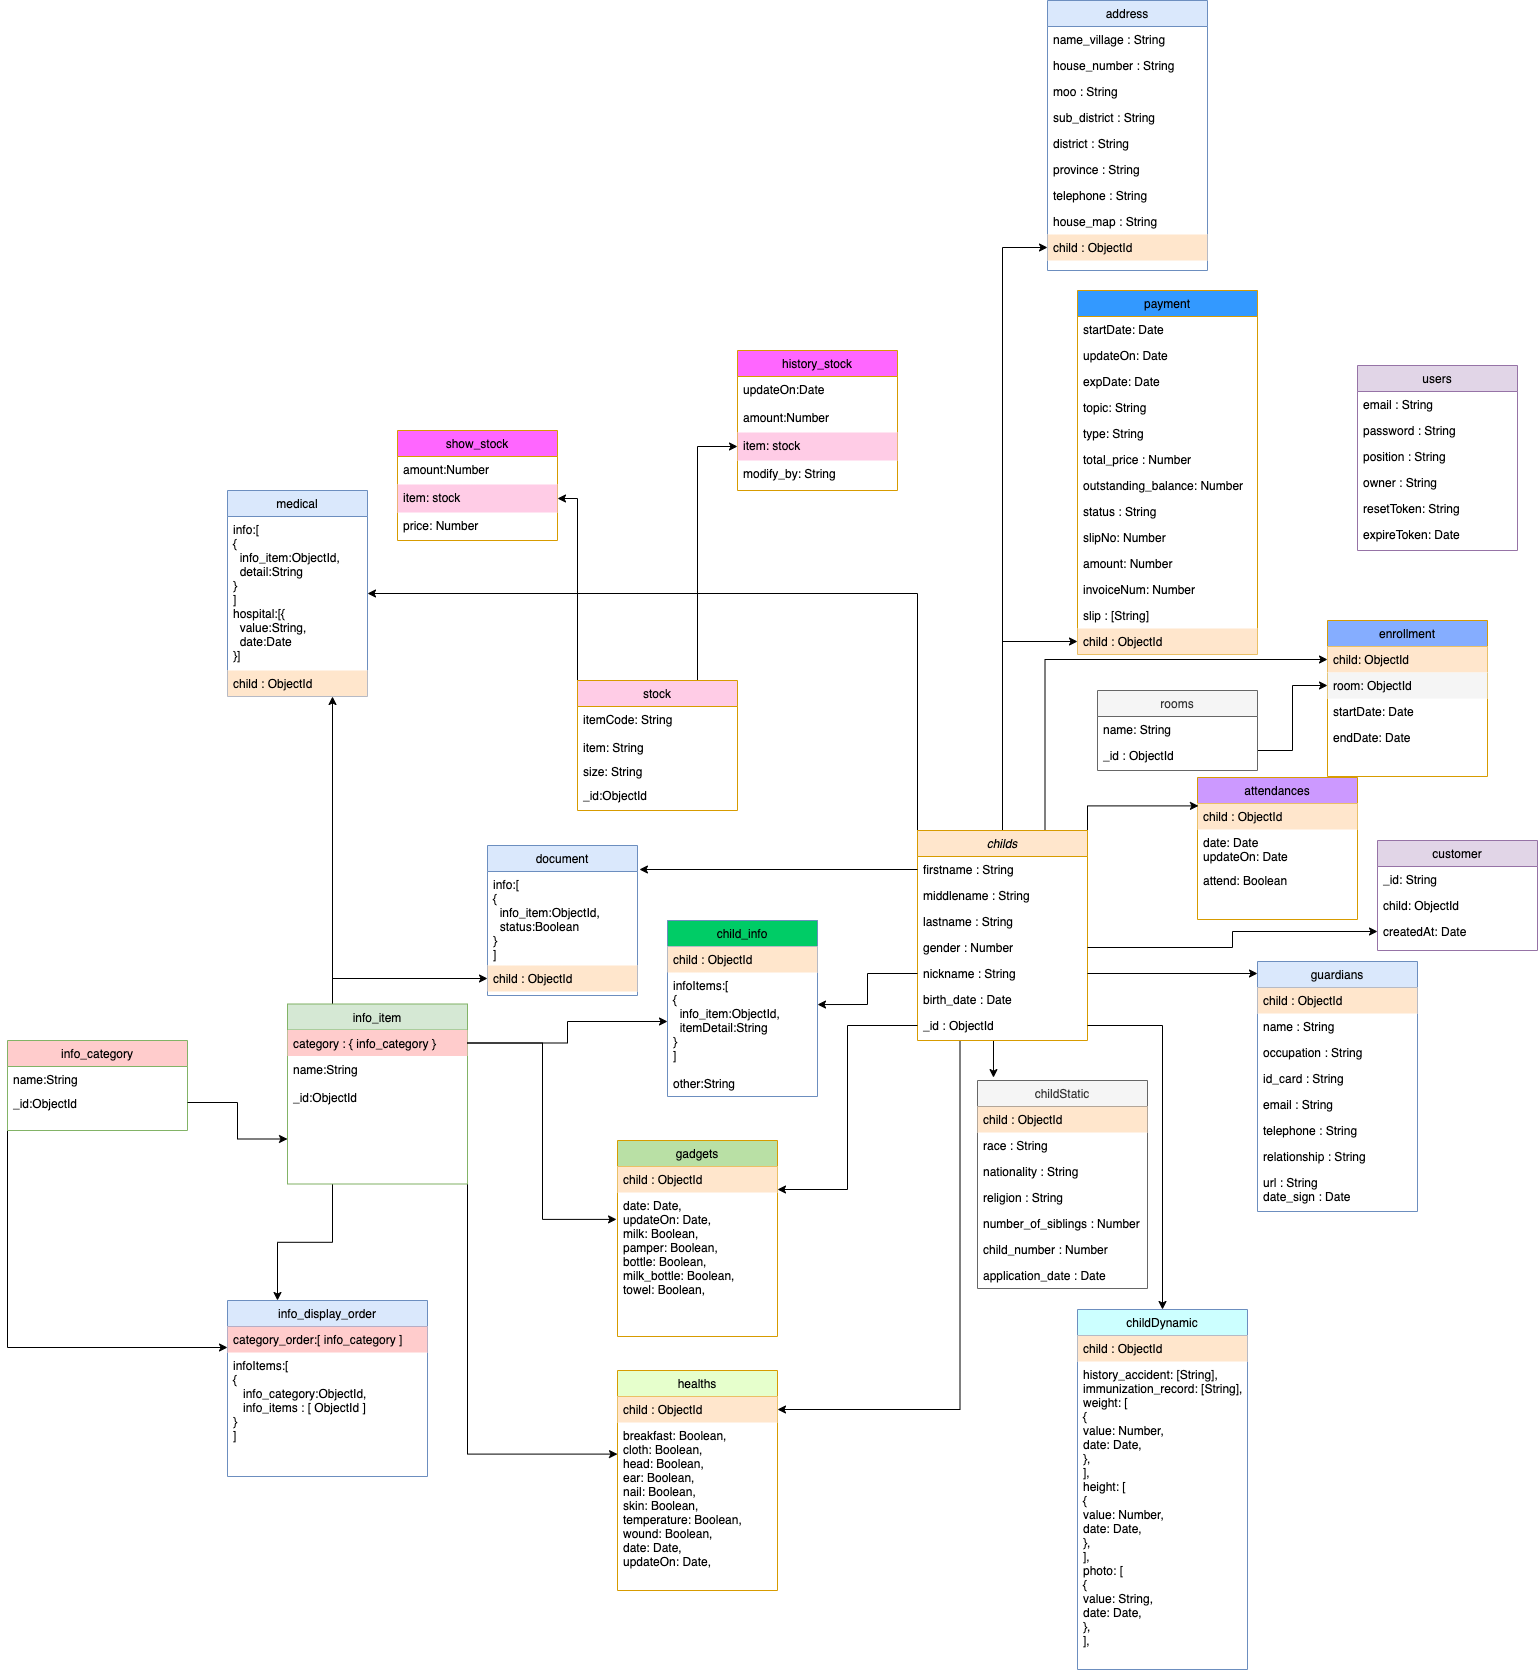
\includegraphics[height=1.0\textheight]{images/NurseryDiagram.png}
    \end{center}
  \caption{แผนภาพแสดงรายละเอียดฐานข้อมูลของระบบ}
  \label{fig:DatabaseDiagram}
\end{figure}
\end{landscape}
  
  \begin{landscape}
    \begin{figure}
      \begin{center}
        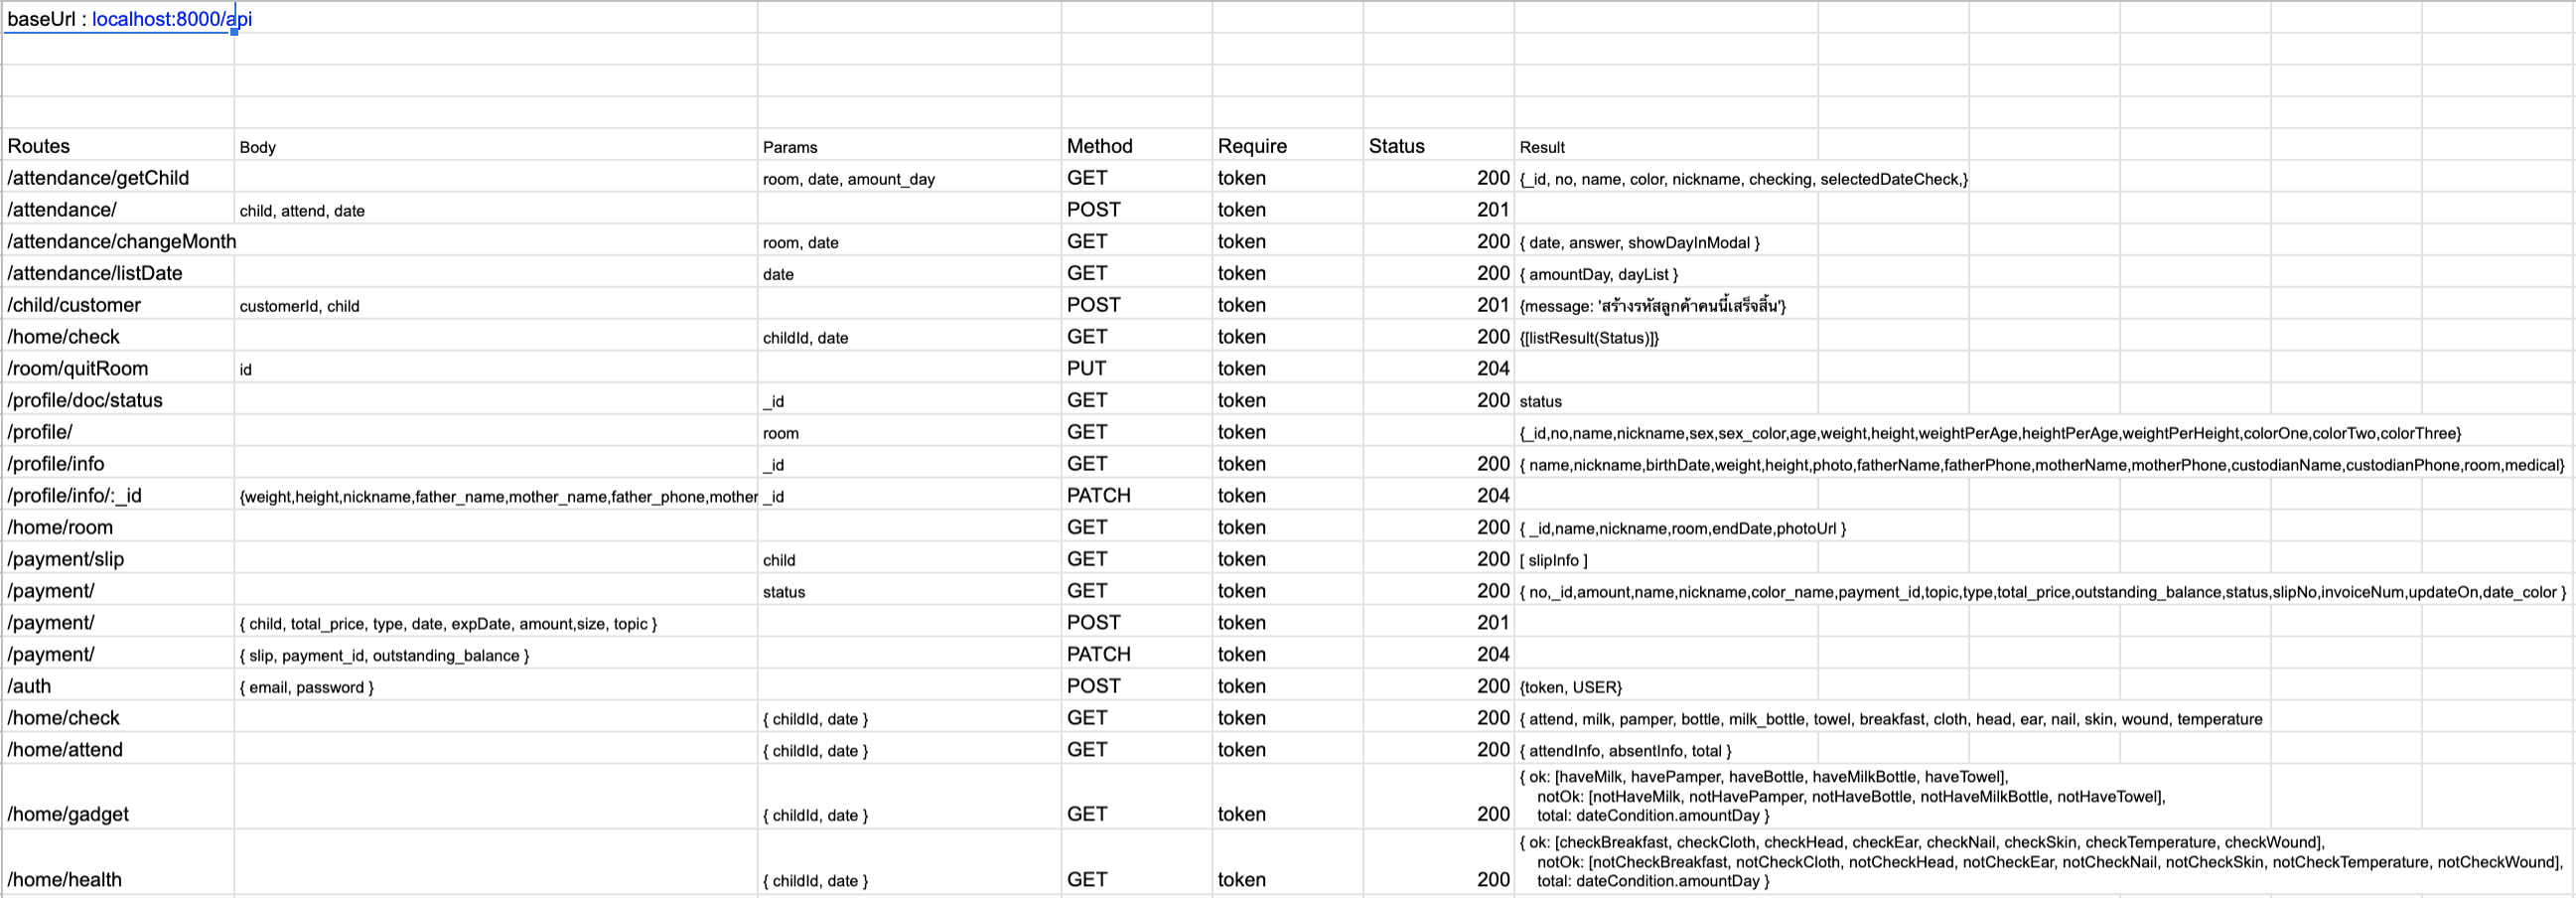
\includegraphics[width=\linewidth]{images/ApiDocOne.png}
      \end{center}
      \caption[ตารางแสดง API Document 1]{ตารางแสดง API Document 1}
      \label{fig:ApiDocs1}
    \end{figure}
  \end{landscape}
  
  \begin{landscape}
    \begin{figure}
      \begin{center}
        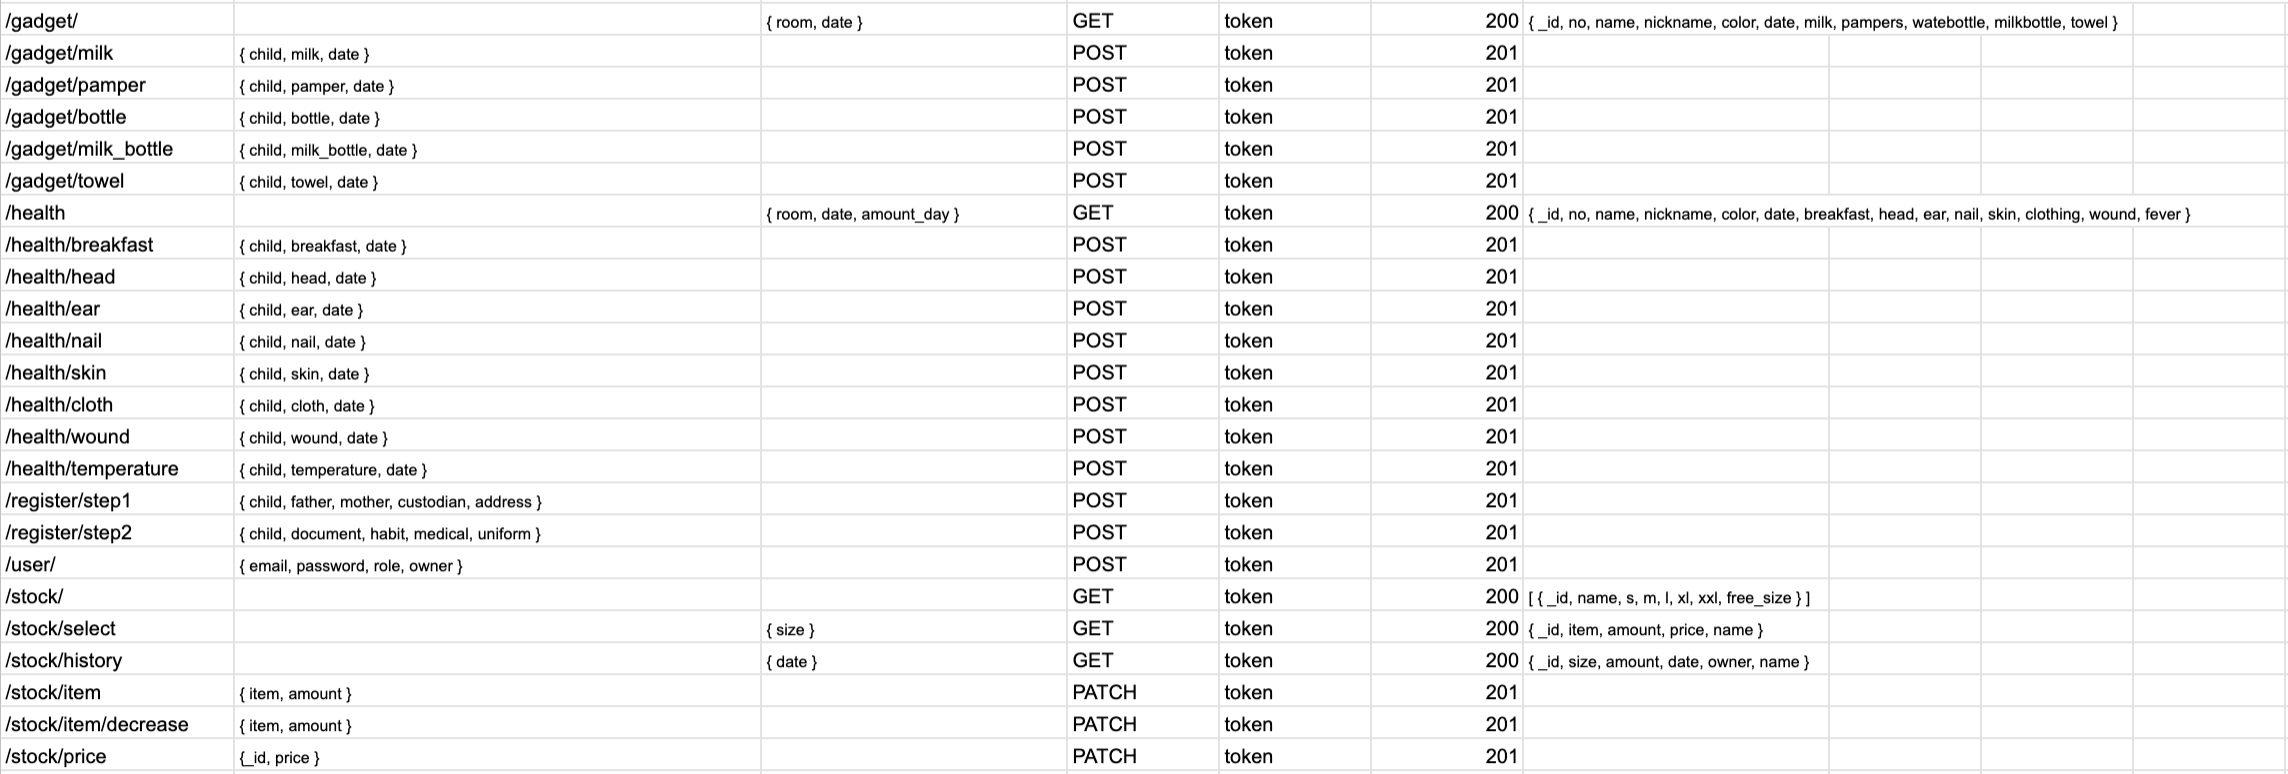
\includegraphics[width=\linewidth]{images/ApiDocTwo.png}
      \end{center}
      \caption[ตารางแสดง API Document 2]{ตารางแสดง API Document 2}
      \label{fig:ApiDocs2}
    \end{figure}
  \end{landscape}

  \begin{figure}
    \begin{center}
    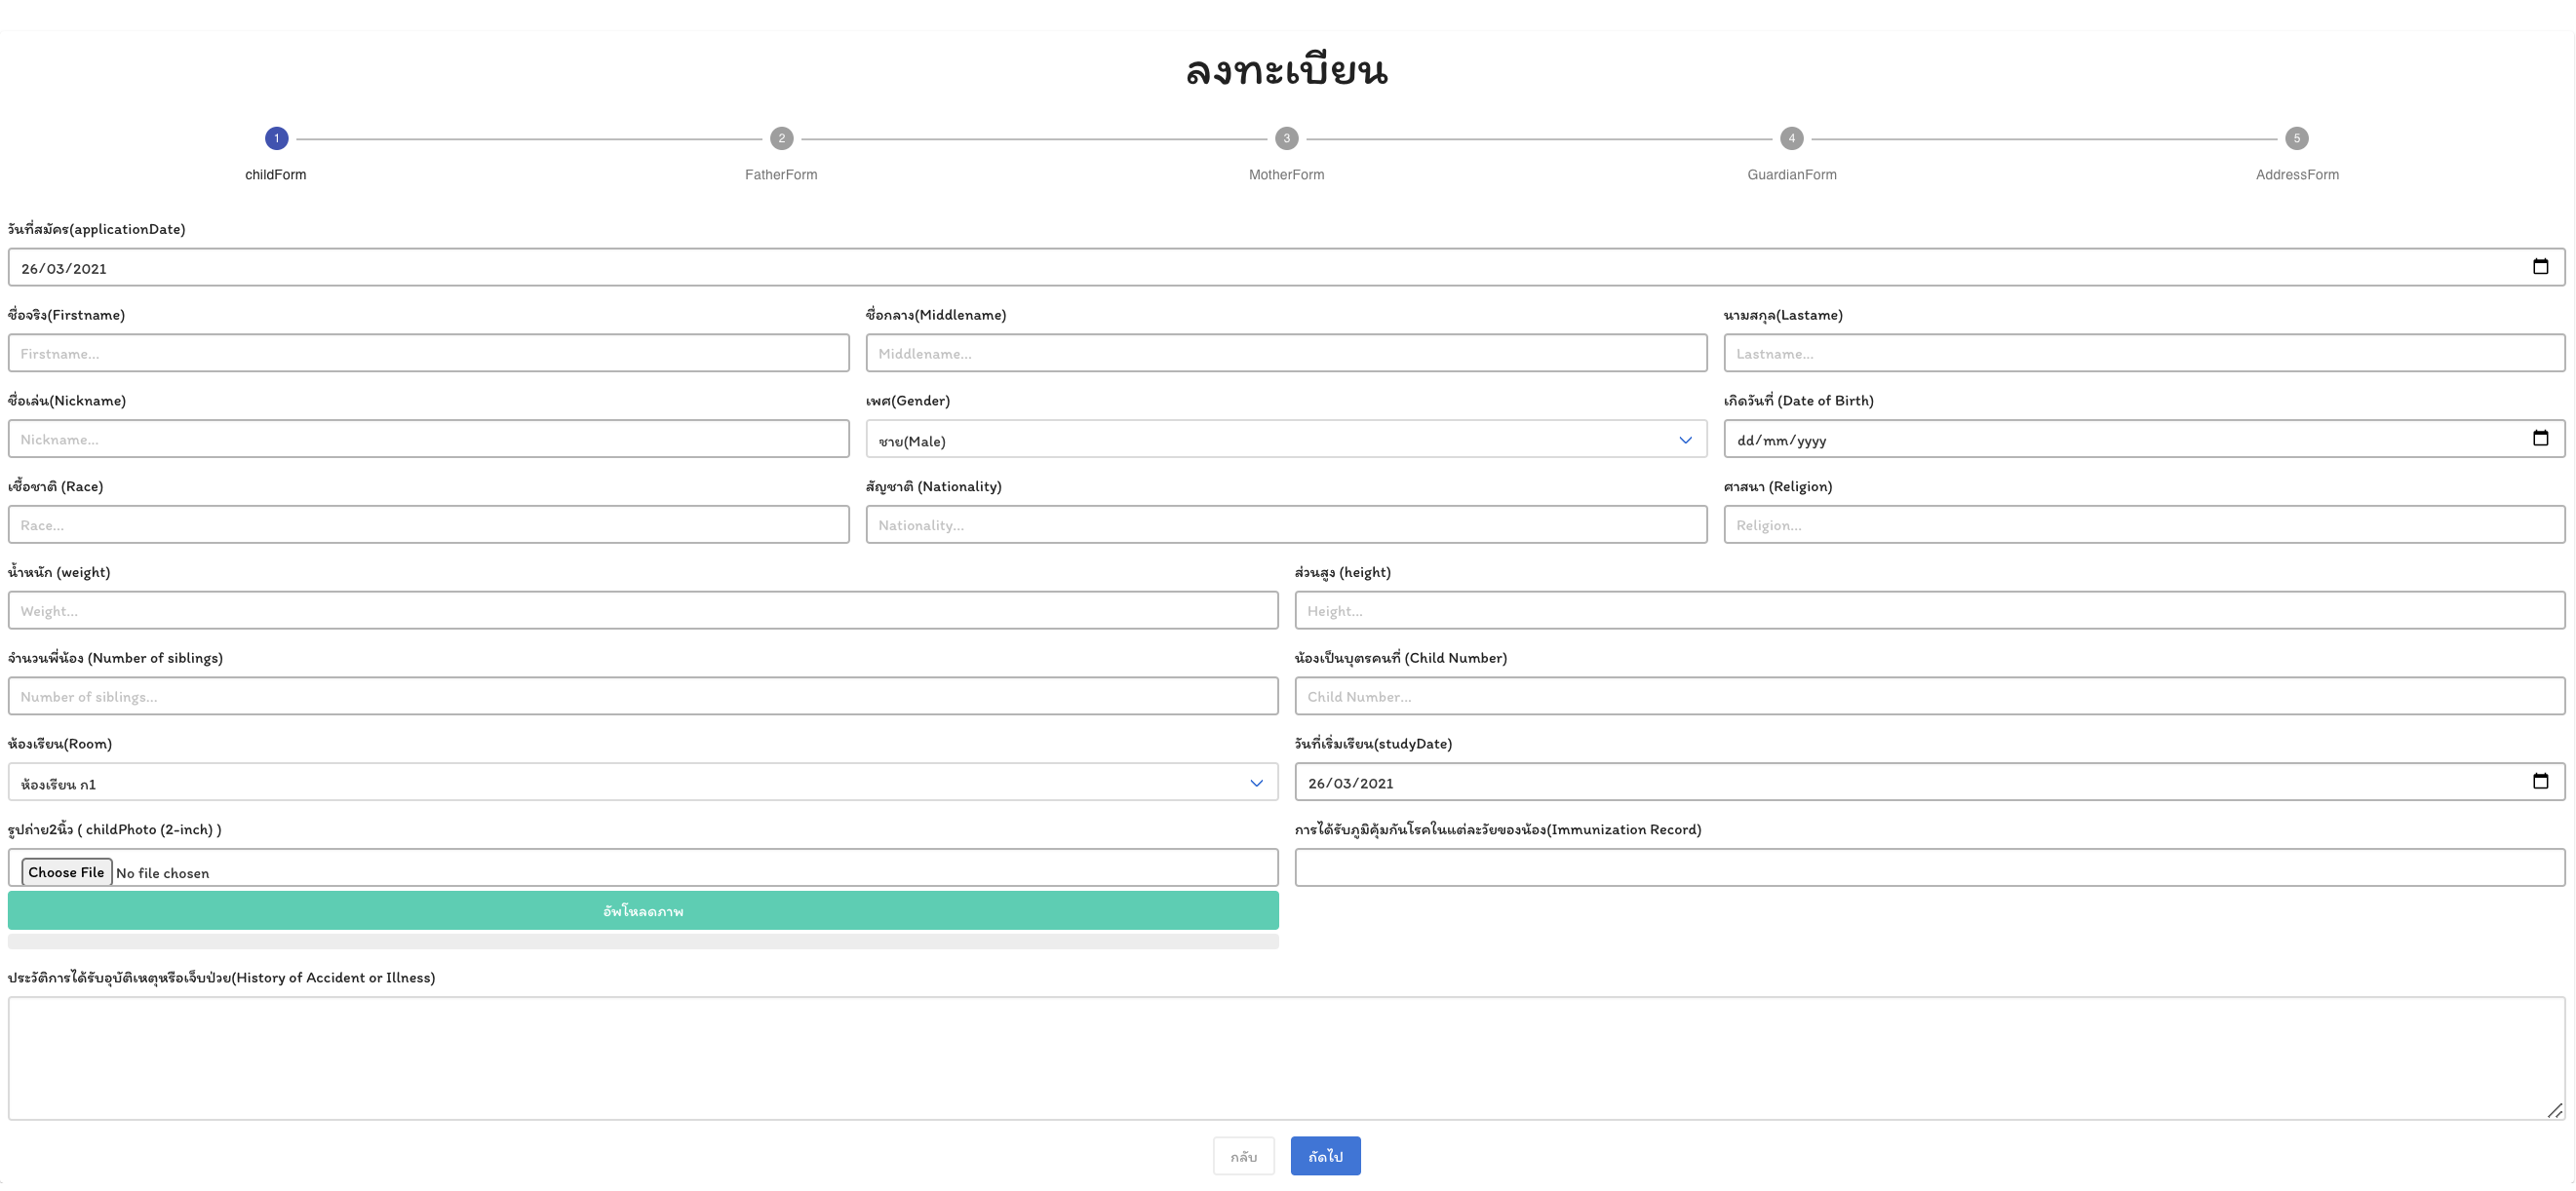
\includegraphics[width=\linewidth]{images/RegisterForm.png}
    \end{center}
    \caption[หน้ากรอกข้อมูลเด็ก]{หน้ากรอกข้อมูลเด็ก}
    \label{fig:register}
  \end{figure}


  \begin{figure}
    \begin{center}
    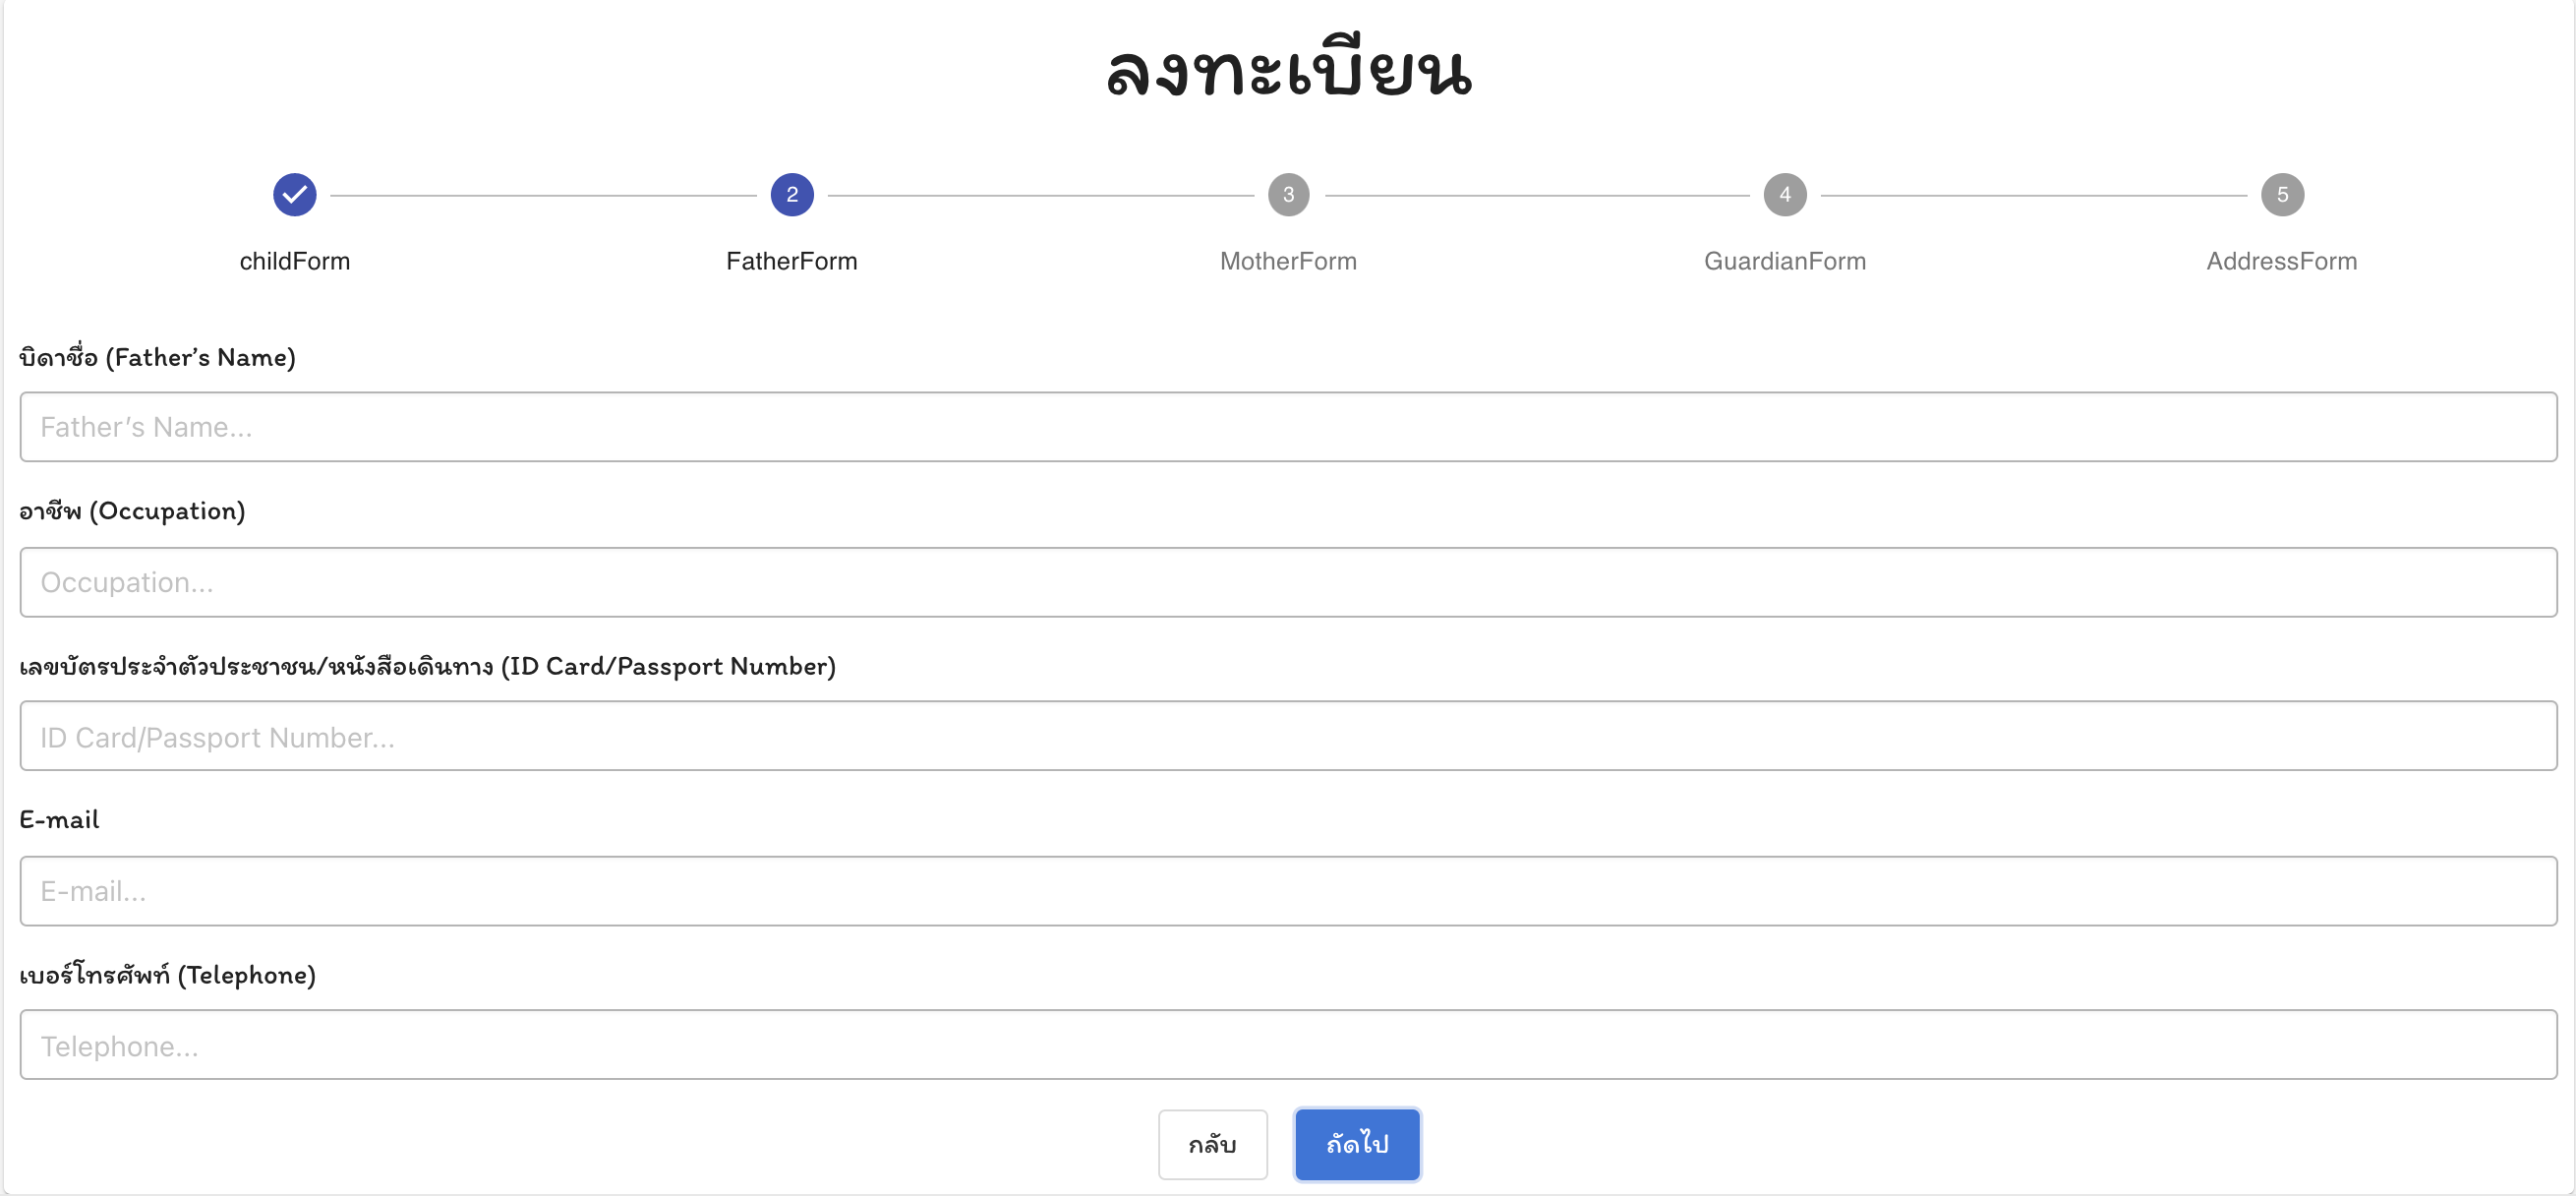
\includegraphics[width=\linewidth]{images/fatherForm.png}
    \end{center}
    \caption[หน้ากรอกข้อมูลบิดา]{หน้ากรอกข้อมูลบิดา}
    \label{fig:fatherForm}
  \end{figure}


  \begin{figure}
    \begin{center}
    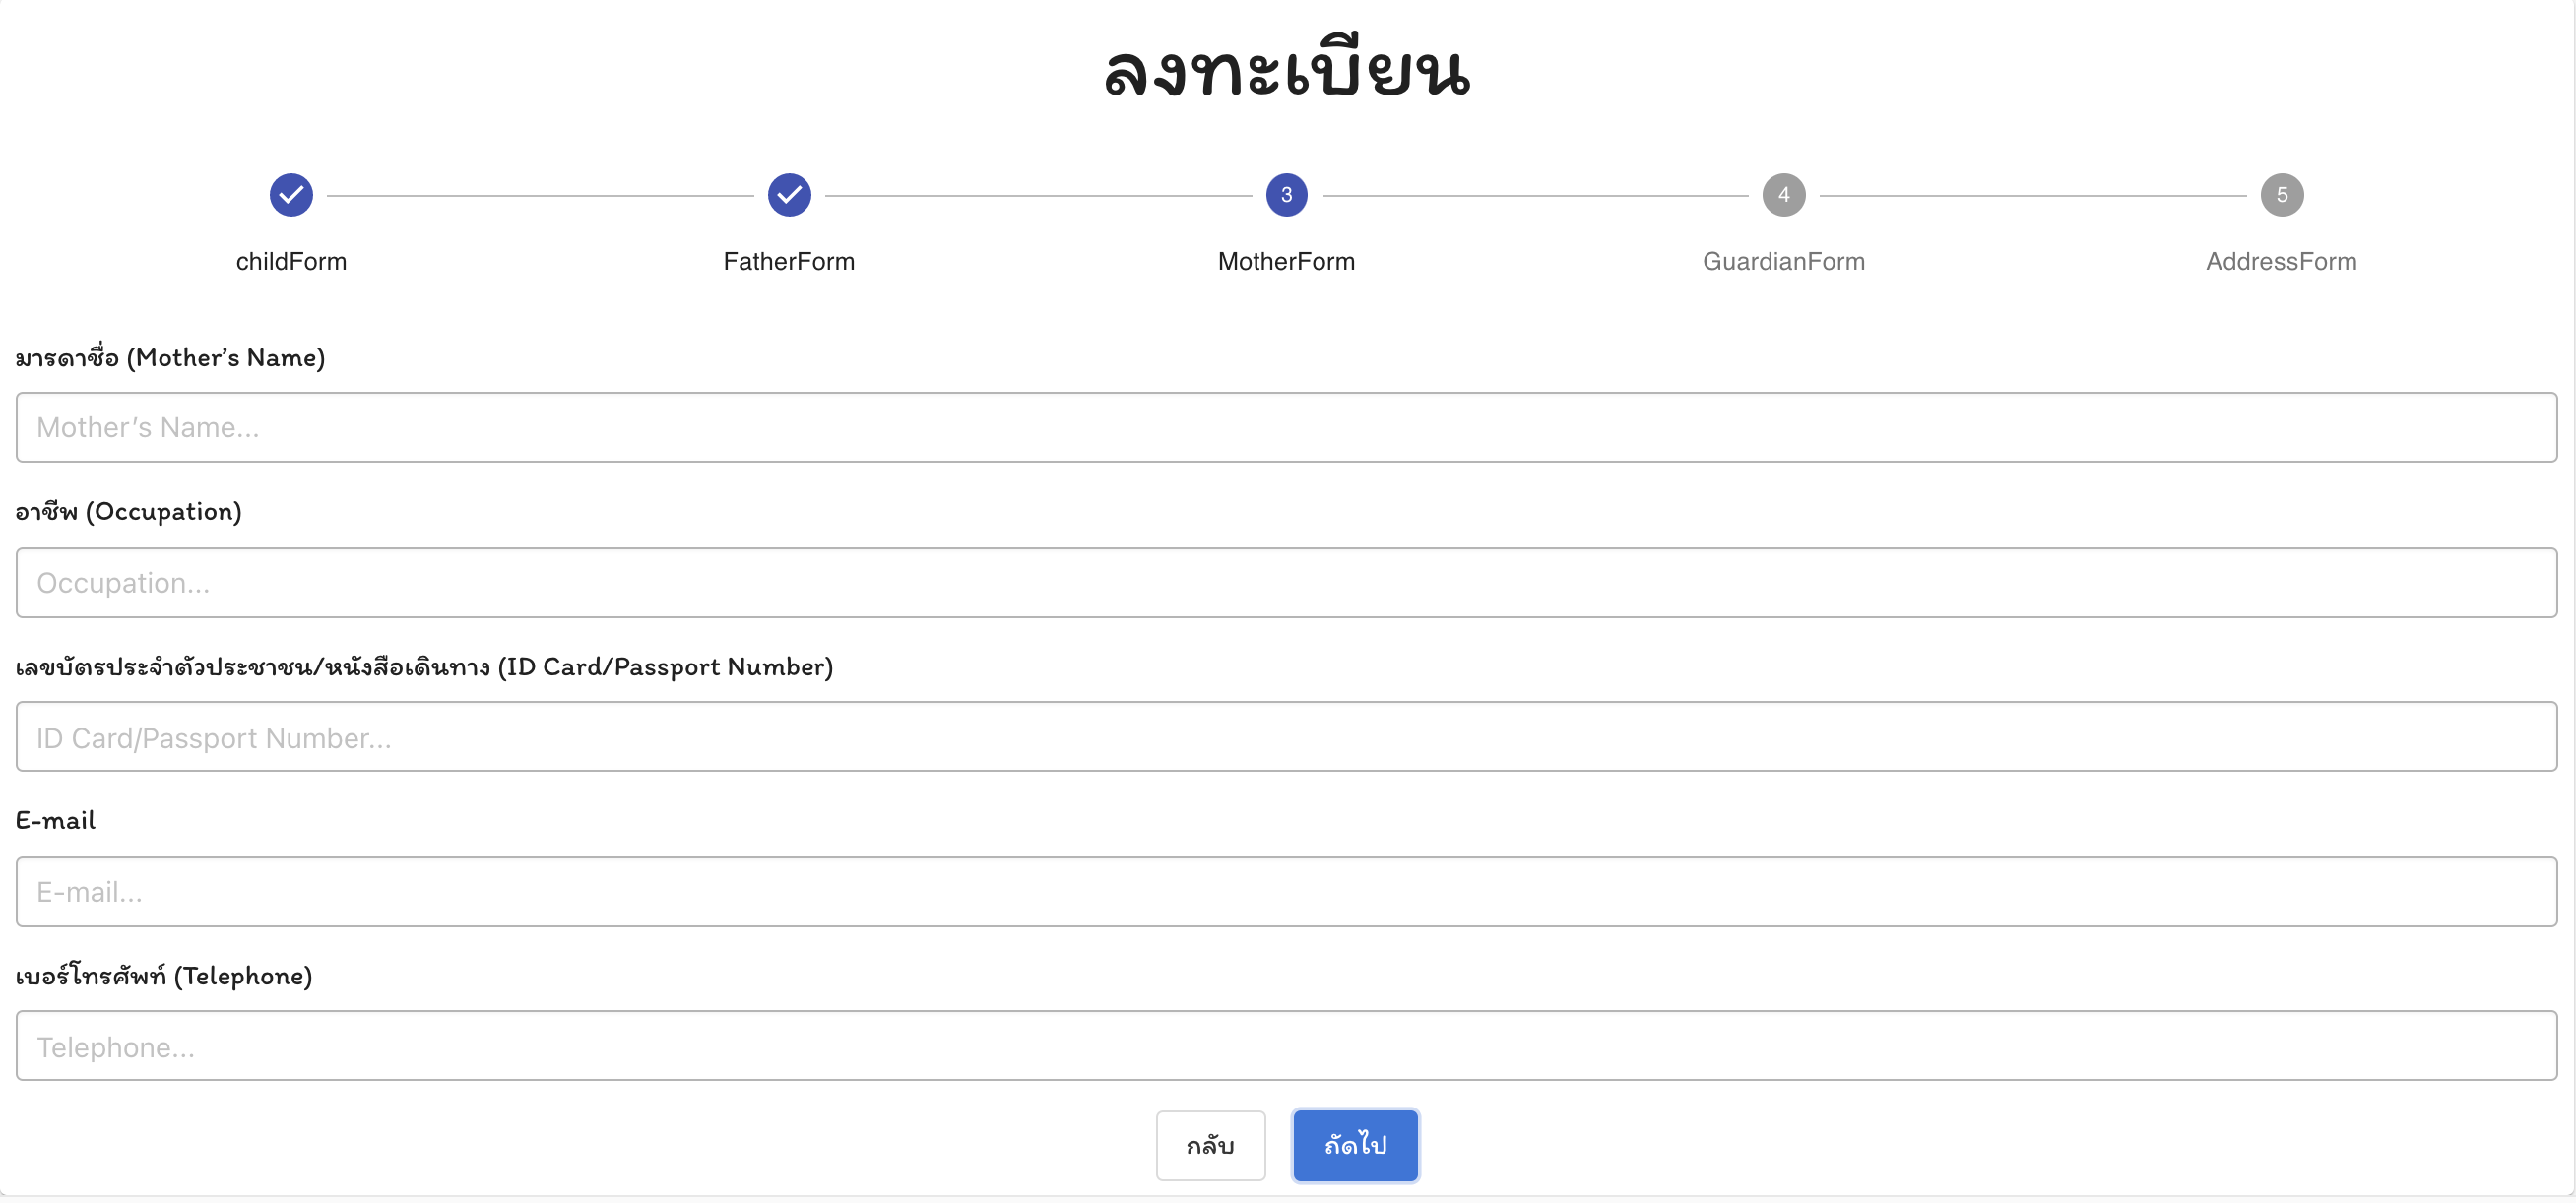
\includegraphics[width=\linewidth]{images/motherForm.png}
    \end{center}
    \caption[หน้ากรอกข้อมูลมารดา]{หน้ากรอกข้อมูลมารดา}
    \label{fig:motherForm}
  \end{figure}


  \begin{figure}
    \begin{center}
    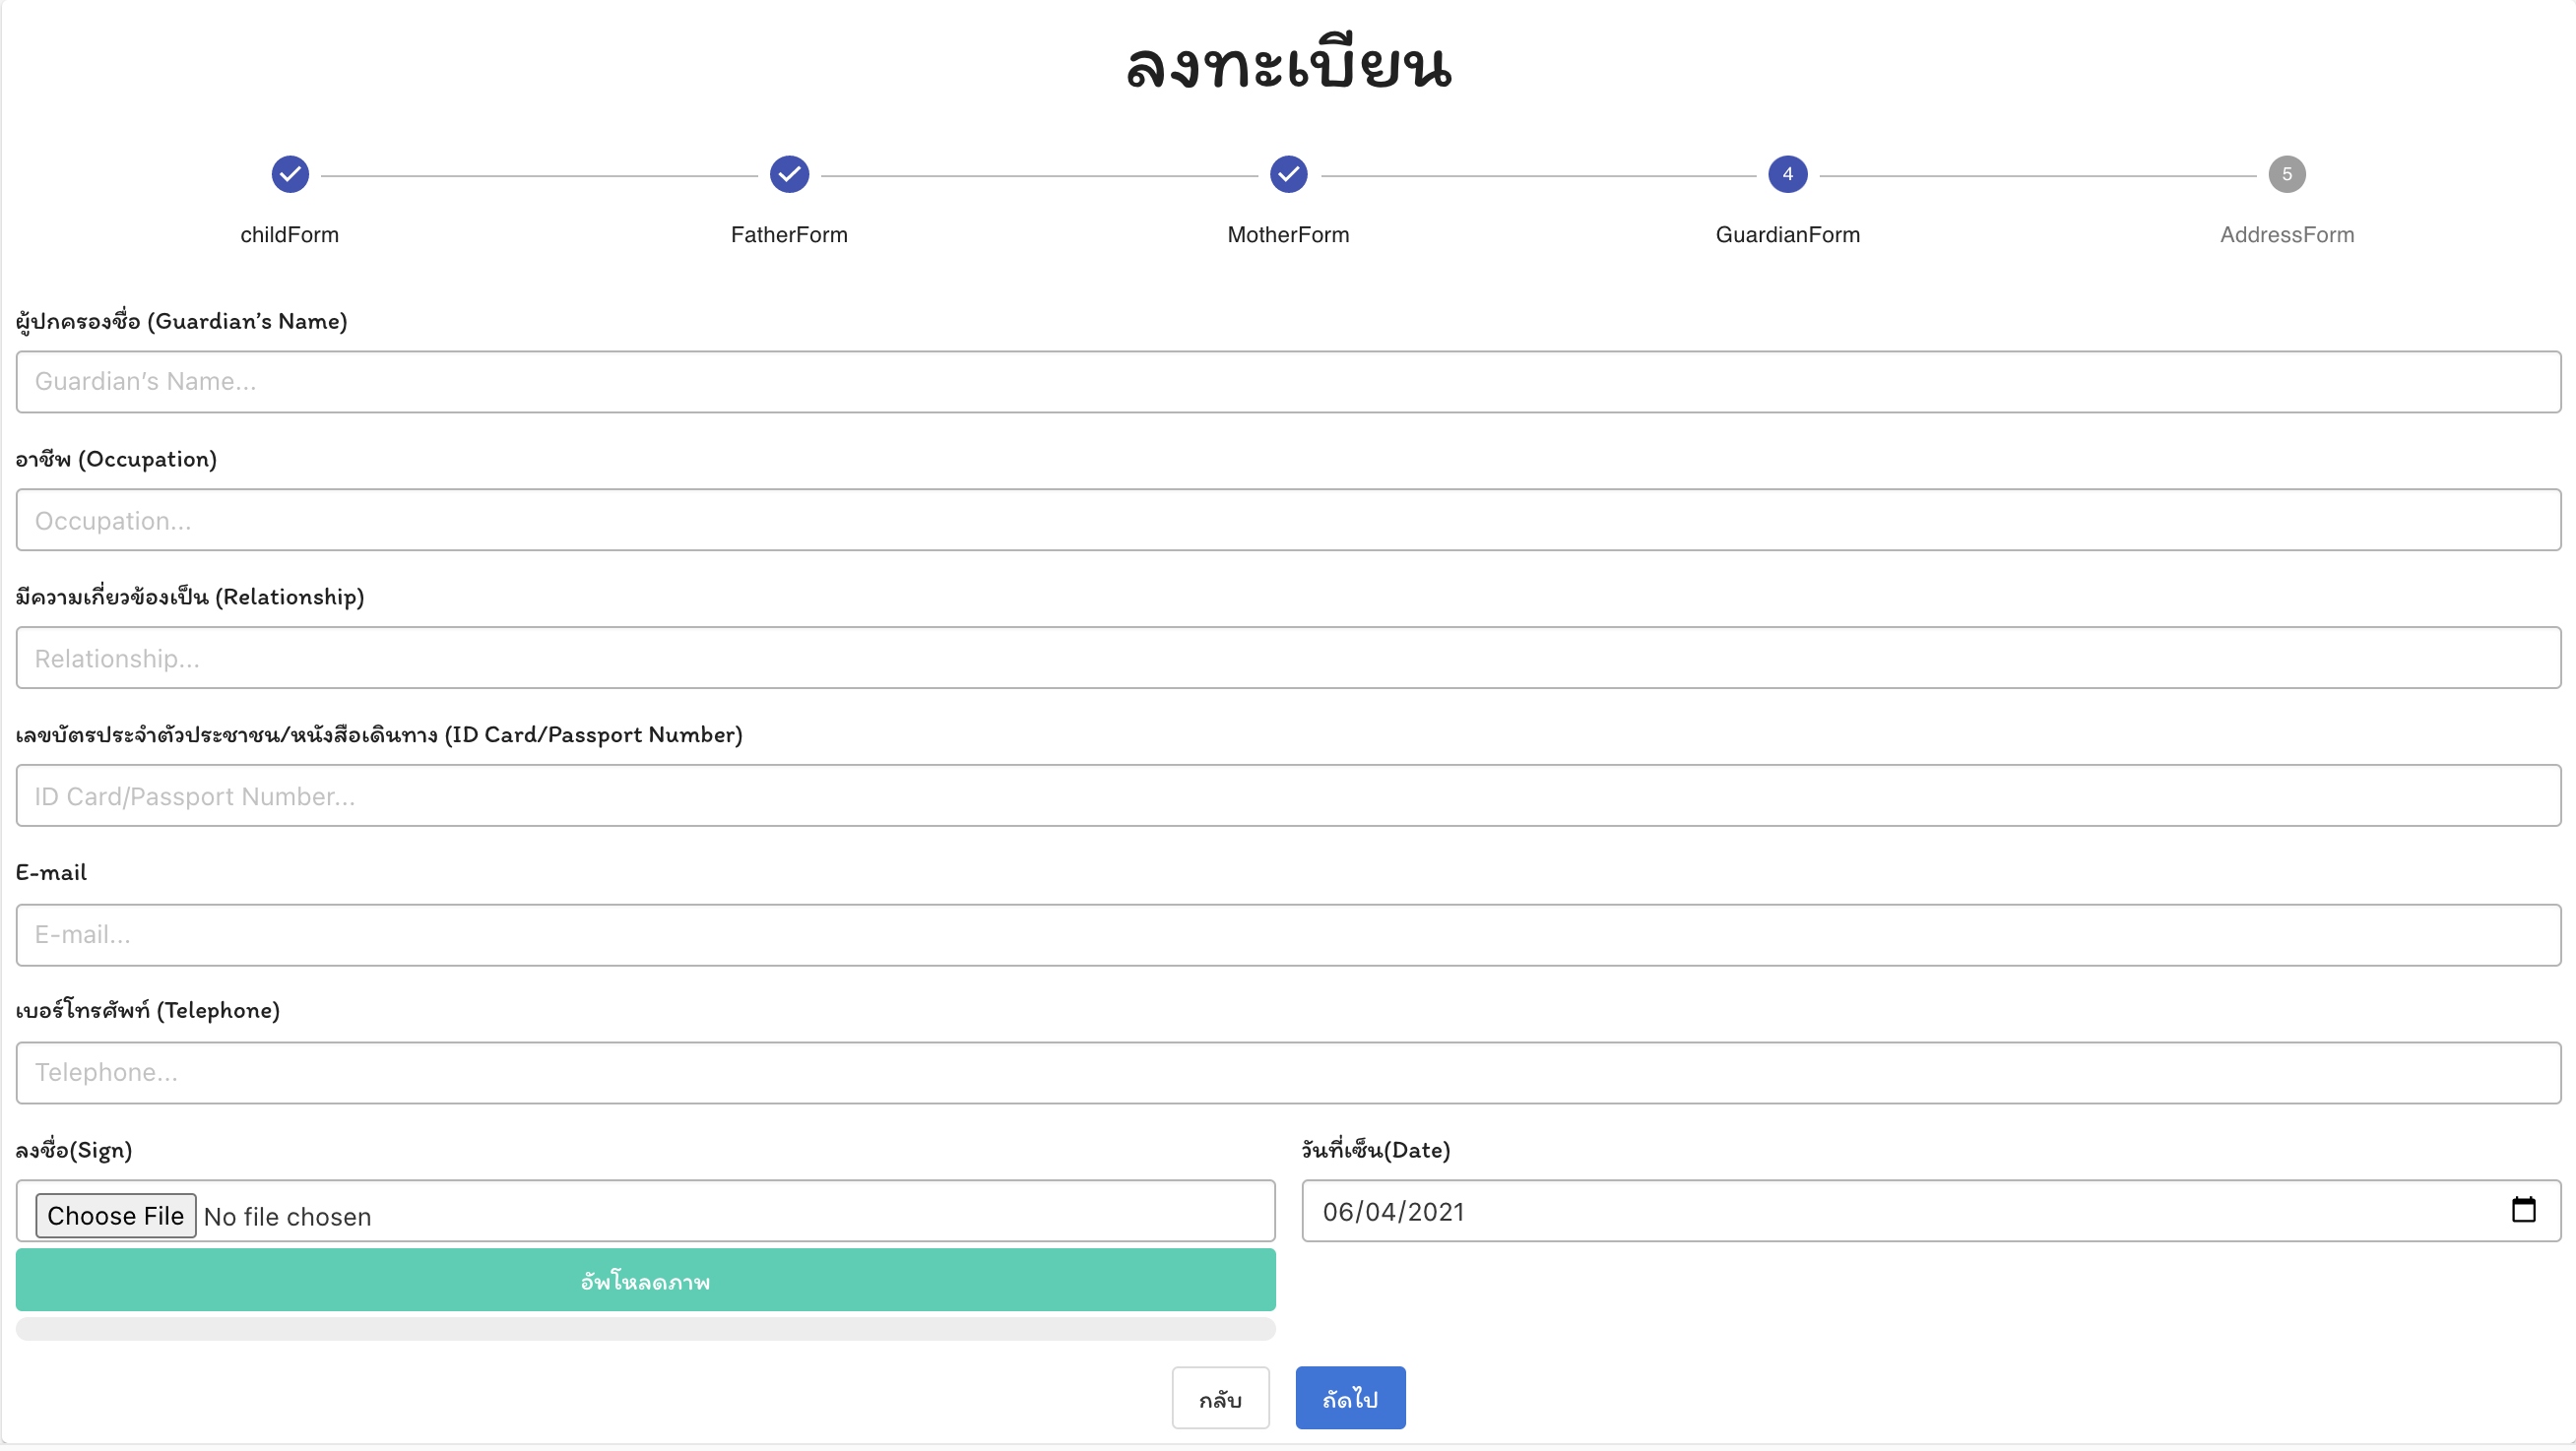
\includegraphics[width=\linewidth]{images/guardiansForm.png}
    \end{center}
    \caption[หน้ากรอกข้อมูลผู้ปกครอง]{หน้ากรอกข้อมูลผู้ปกครอง}
    \label{fig:guardiansForm}
  \end{figure}


  \begin{figure}
    \begin{center}
    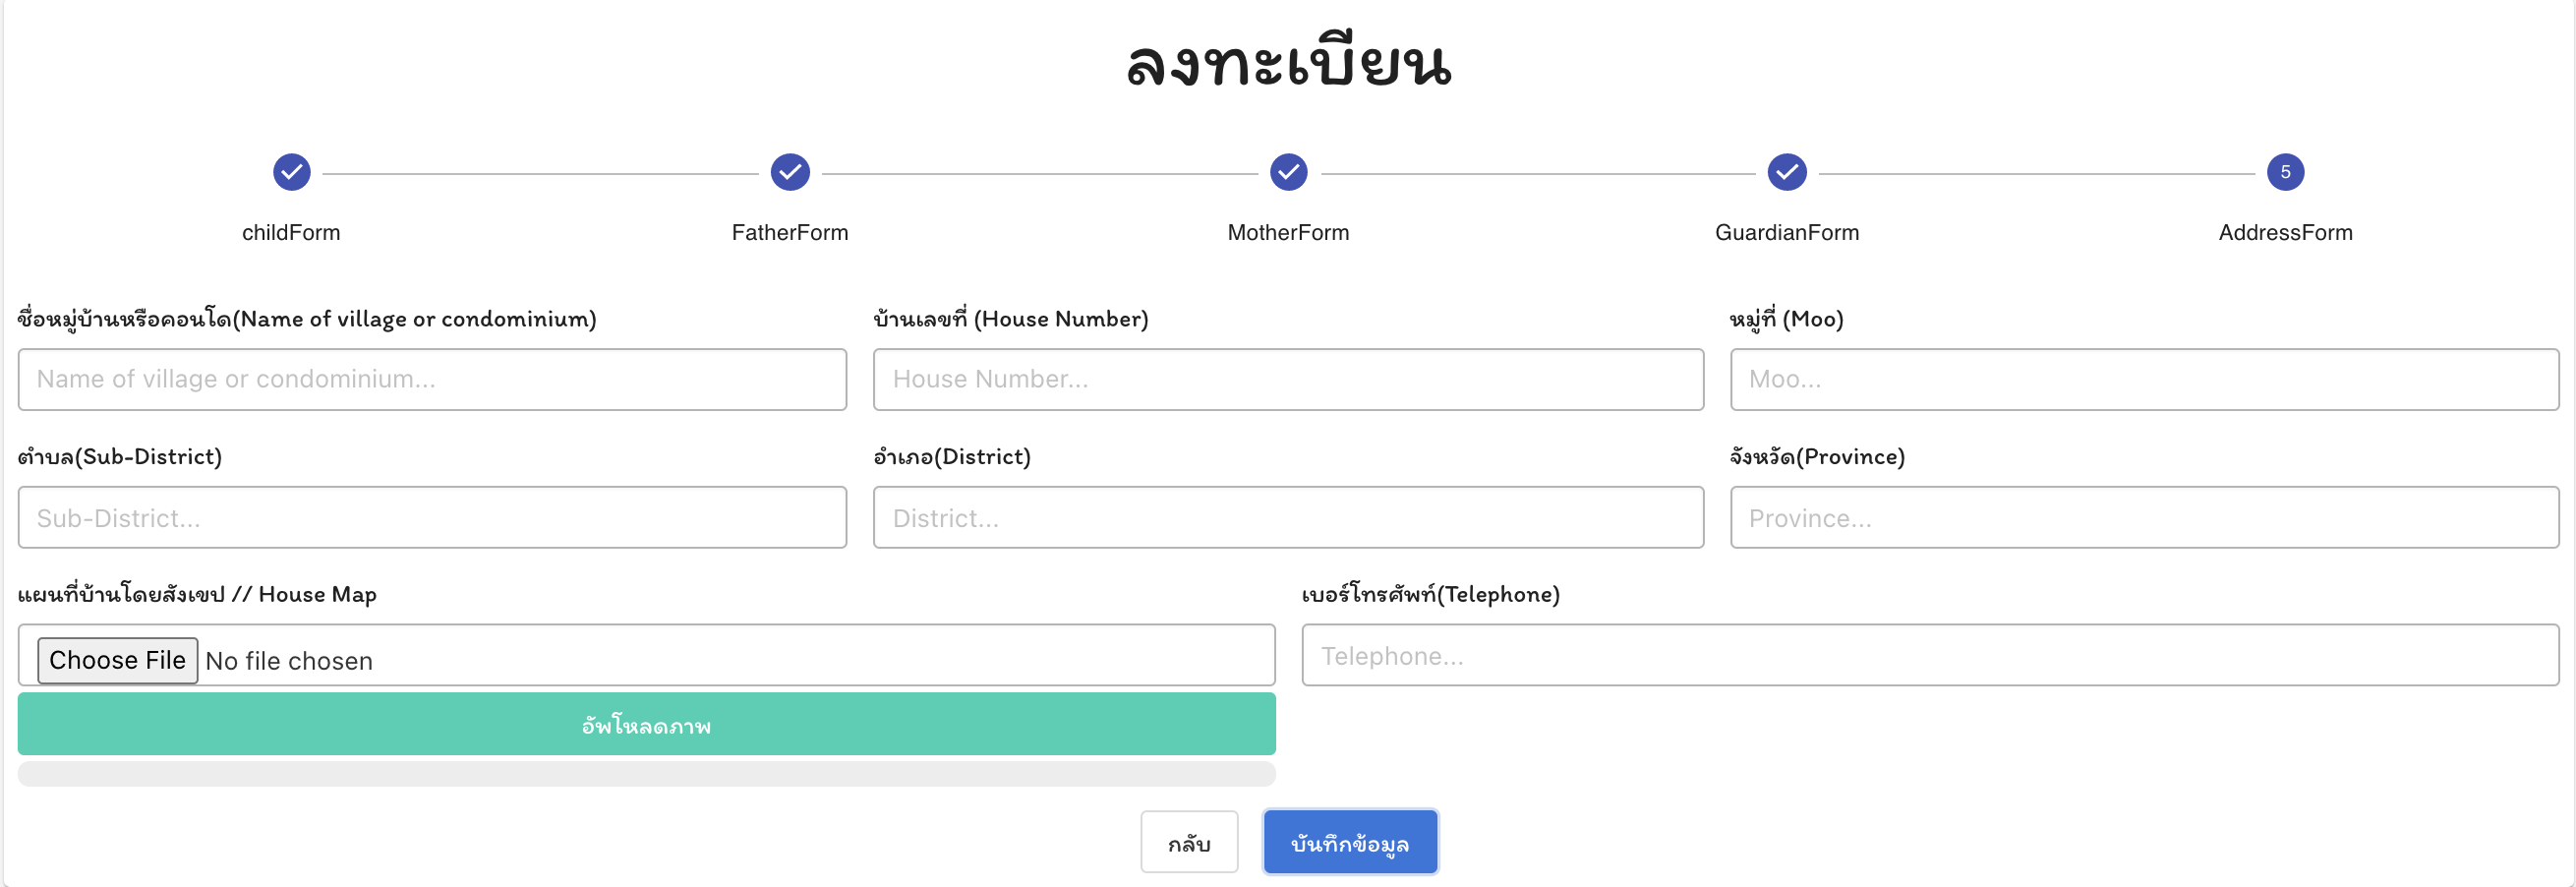
\includegraphics[width=\linewidth]{images/addressForm.png}
    \end{center}
    \caption[หน้ากรอกข้อมูลที่อยู่]{หน้ากรอกข้อมูลที่อยู่}
    \label{fig:addressForm}
  \end{figure}

  \begin{figure}
    \begin{center}
    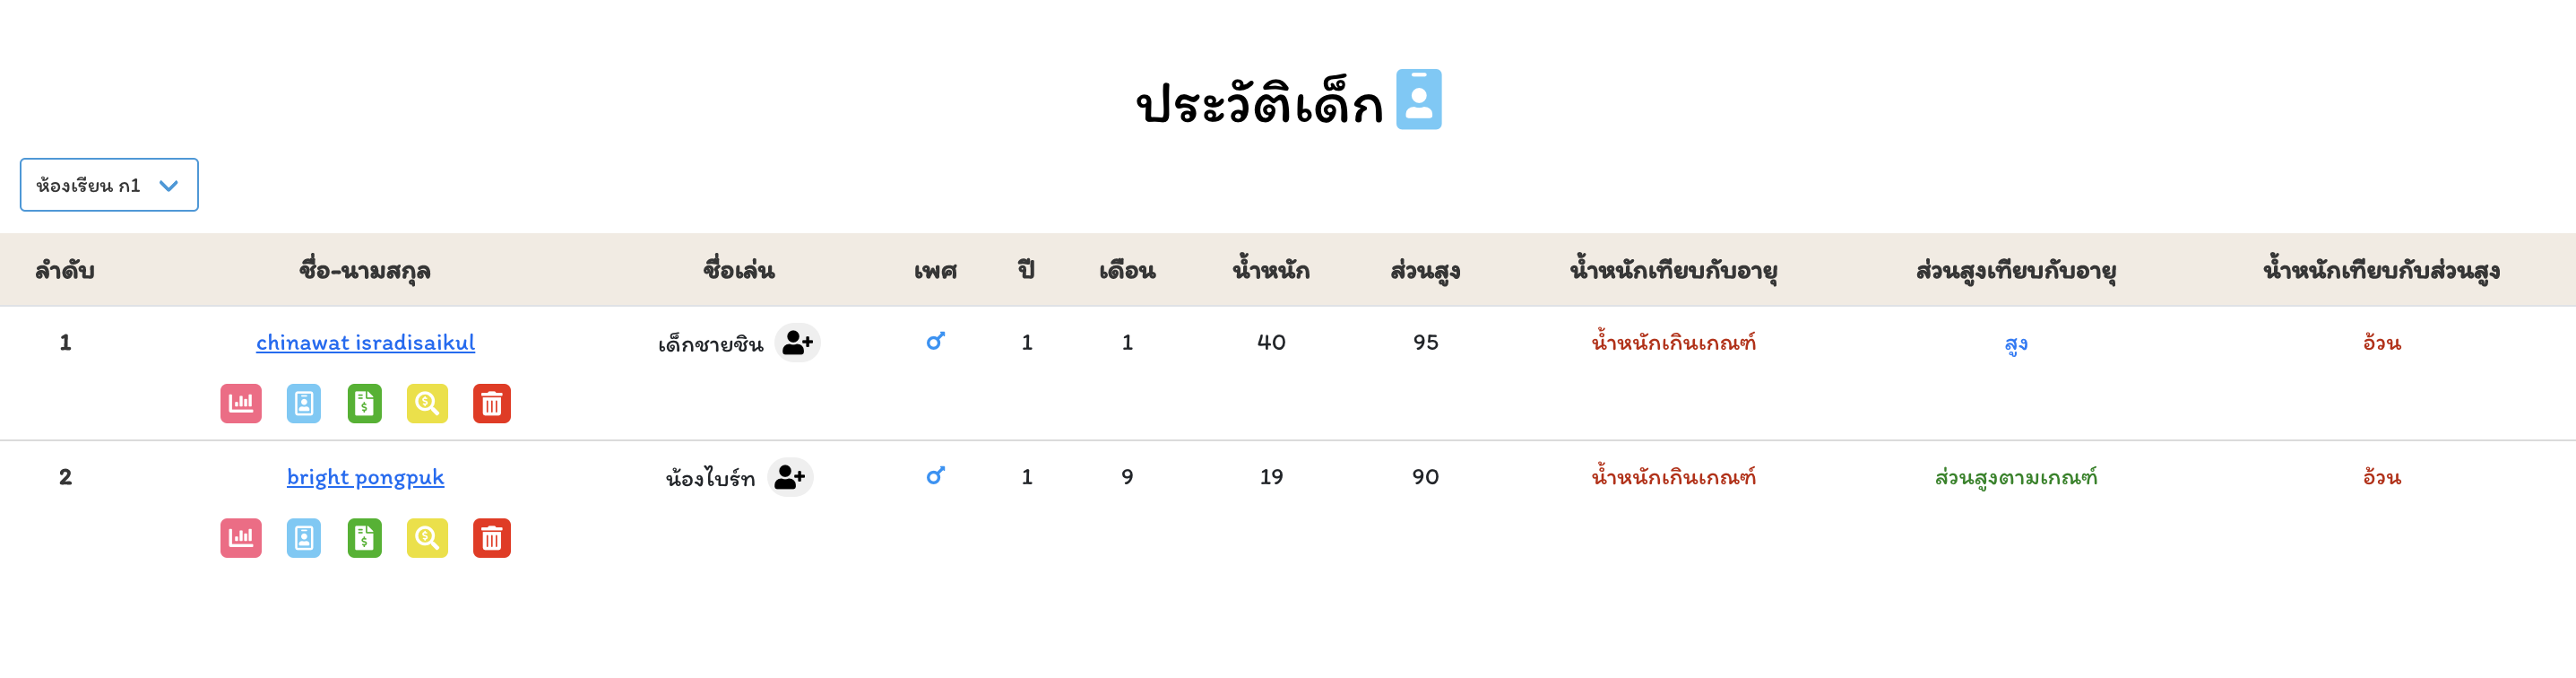
\includegraphics[width=\linewidth]{images/Profile.png}
    \end{center}
    \caption[หน้าประวัติเด็ก]{หน้าประวัติเด็ก}
    \label{fig:Profile}
  \end{figure}



  \begin{figure}
    \begin{center}
    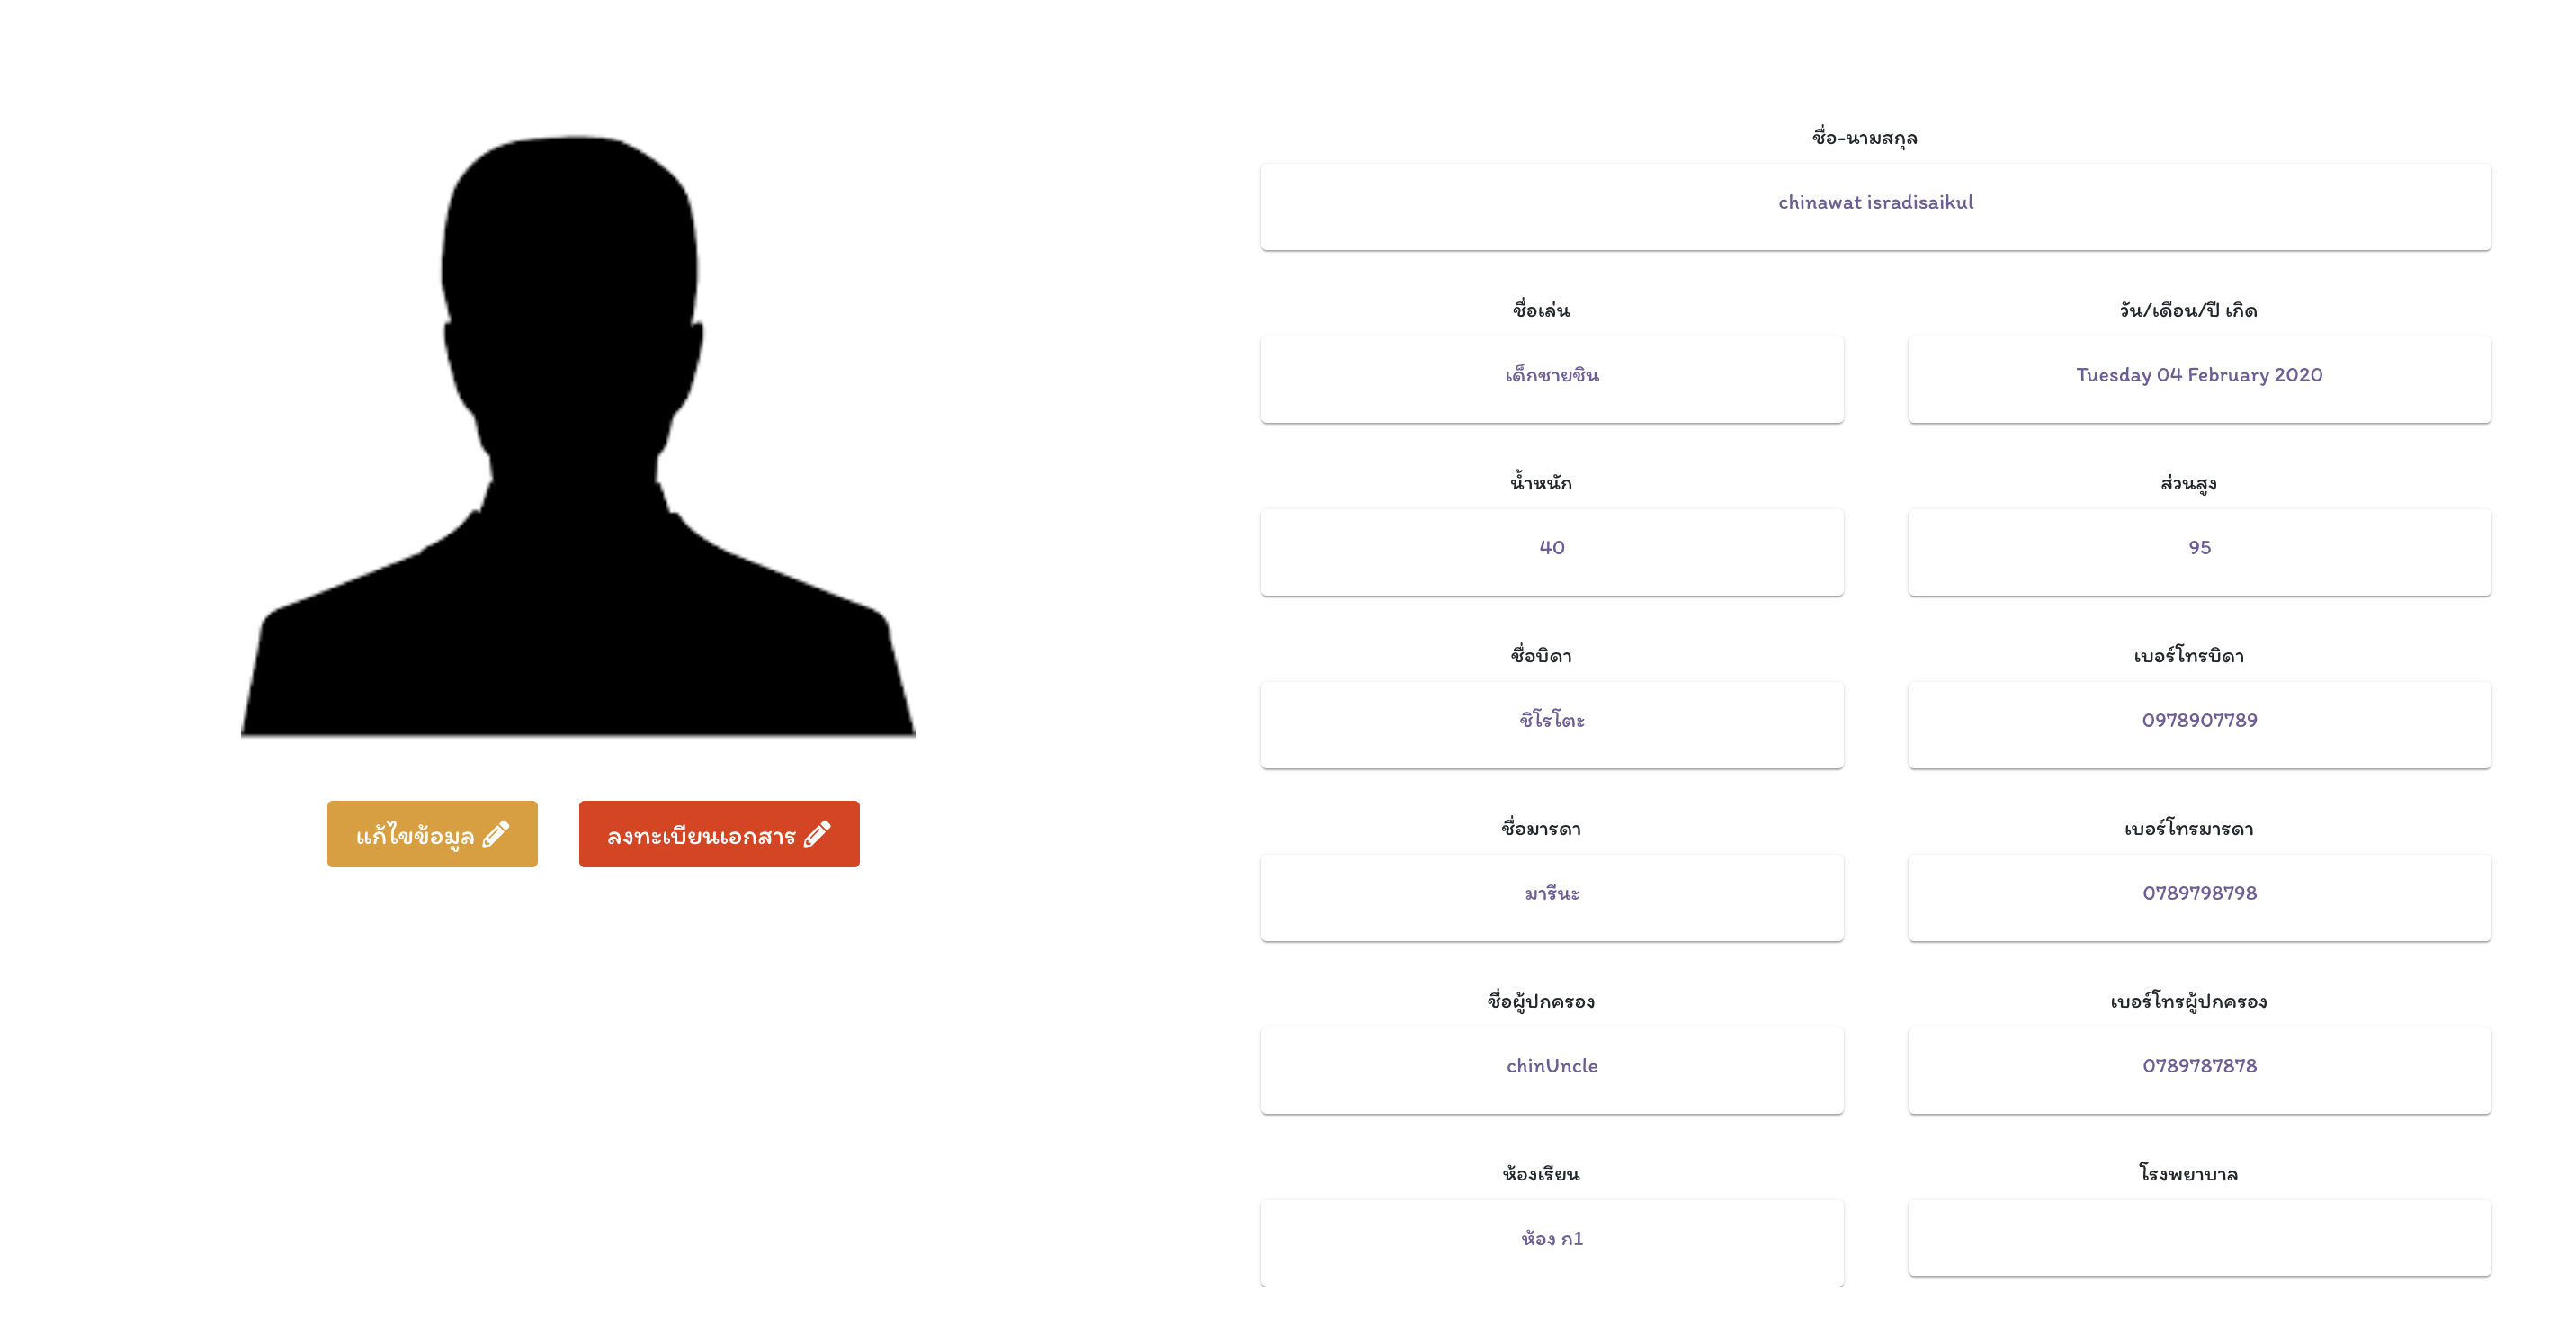
\includegraphics[width=\linewidth]{images/ProfileInfo.png}
    \end{center}
    \caption[หน้าประวัติส่วนตัวเด็ก]{หน้าประวัติส่วนตัวเด็ก}
    \label{fig:ProfileTwo}
  \end{figure}


  \begin{figure}
    \begin{center}
    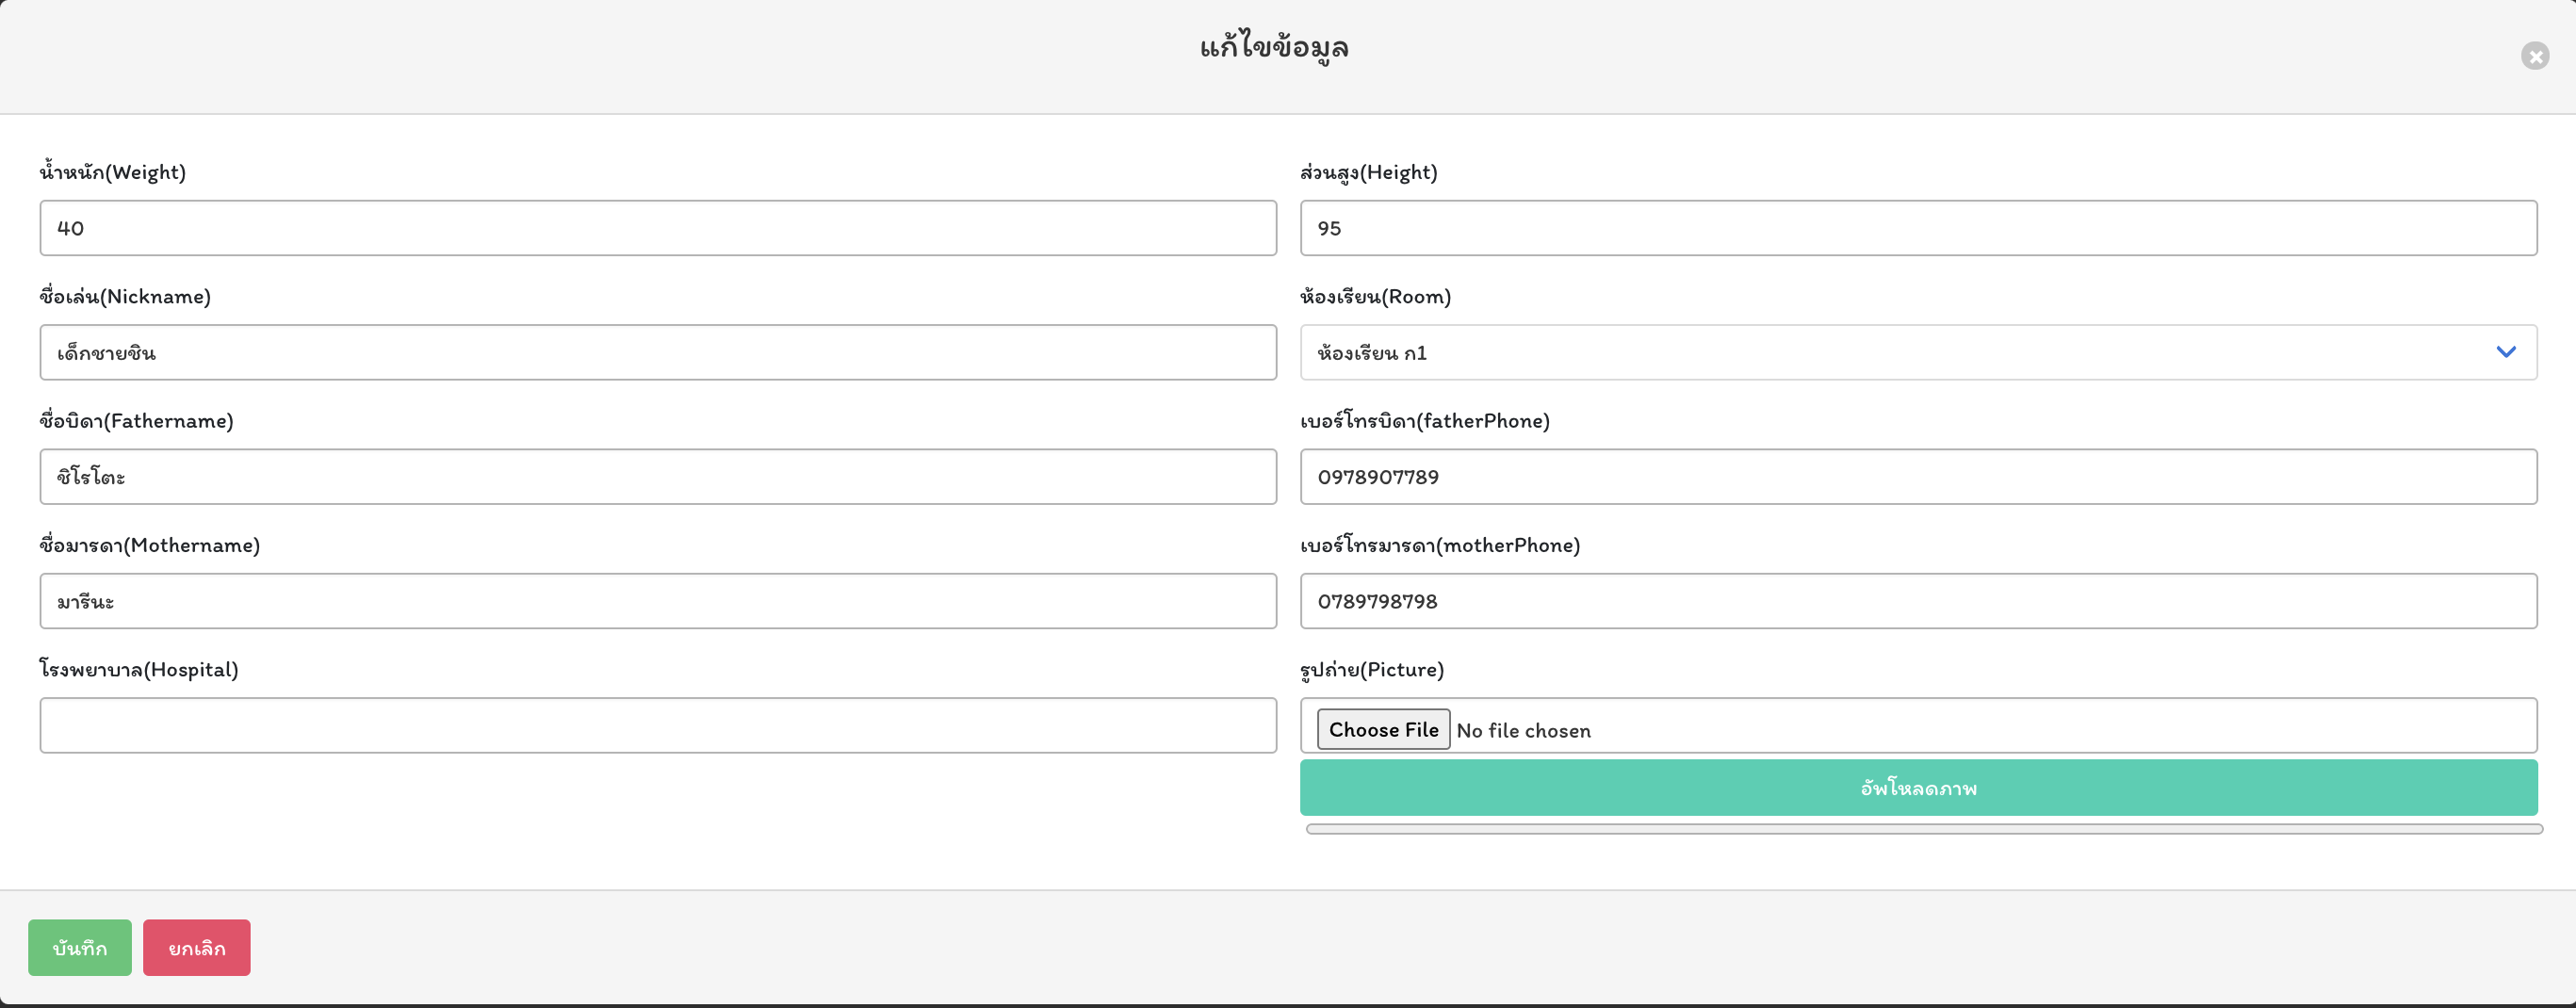
\includegraphics[width=\linewidth]{images/updateProfile.png}
    \end{center}
    \caption[หน้าแก้ไขข้อมูลเด็ก]{หน้าแก้ไขข้อมูลเด็ก}
    \label{fig:UpdateProfile}
    \end{figure}



  \begin{figure}
    \begin{center}
    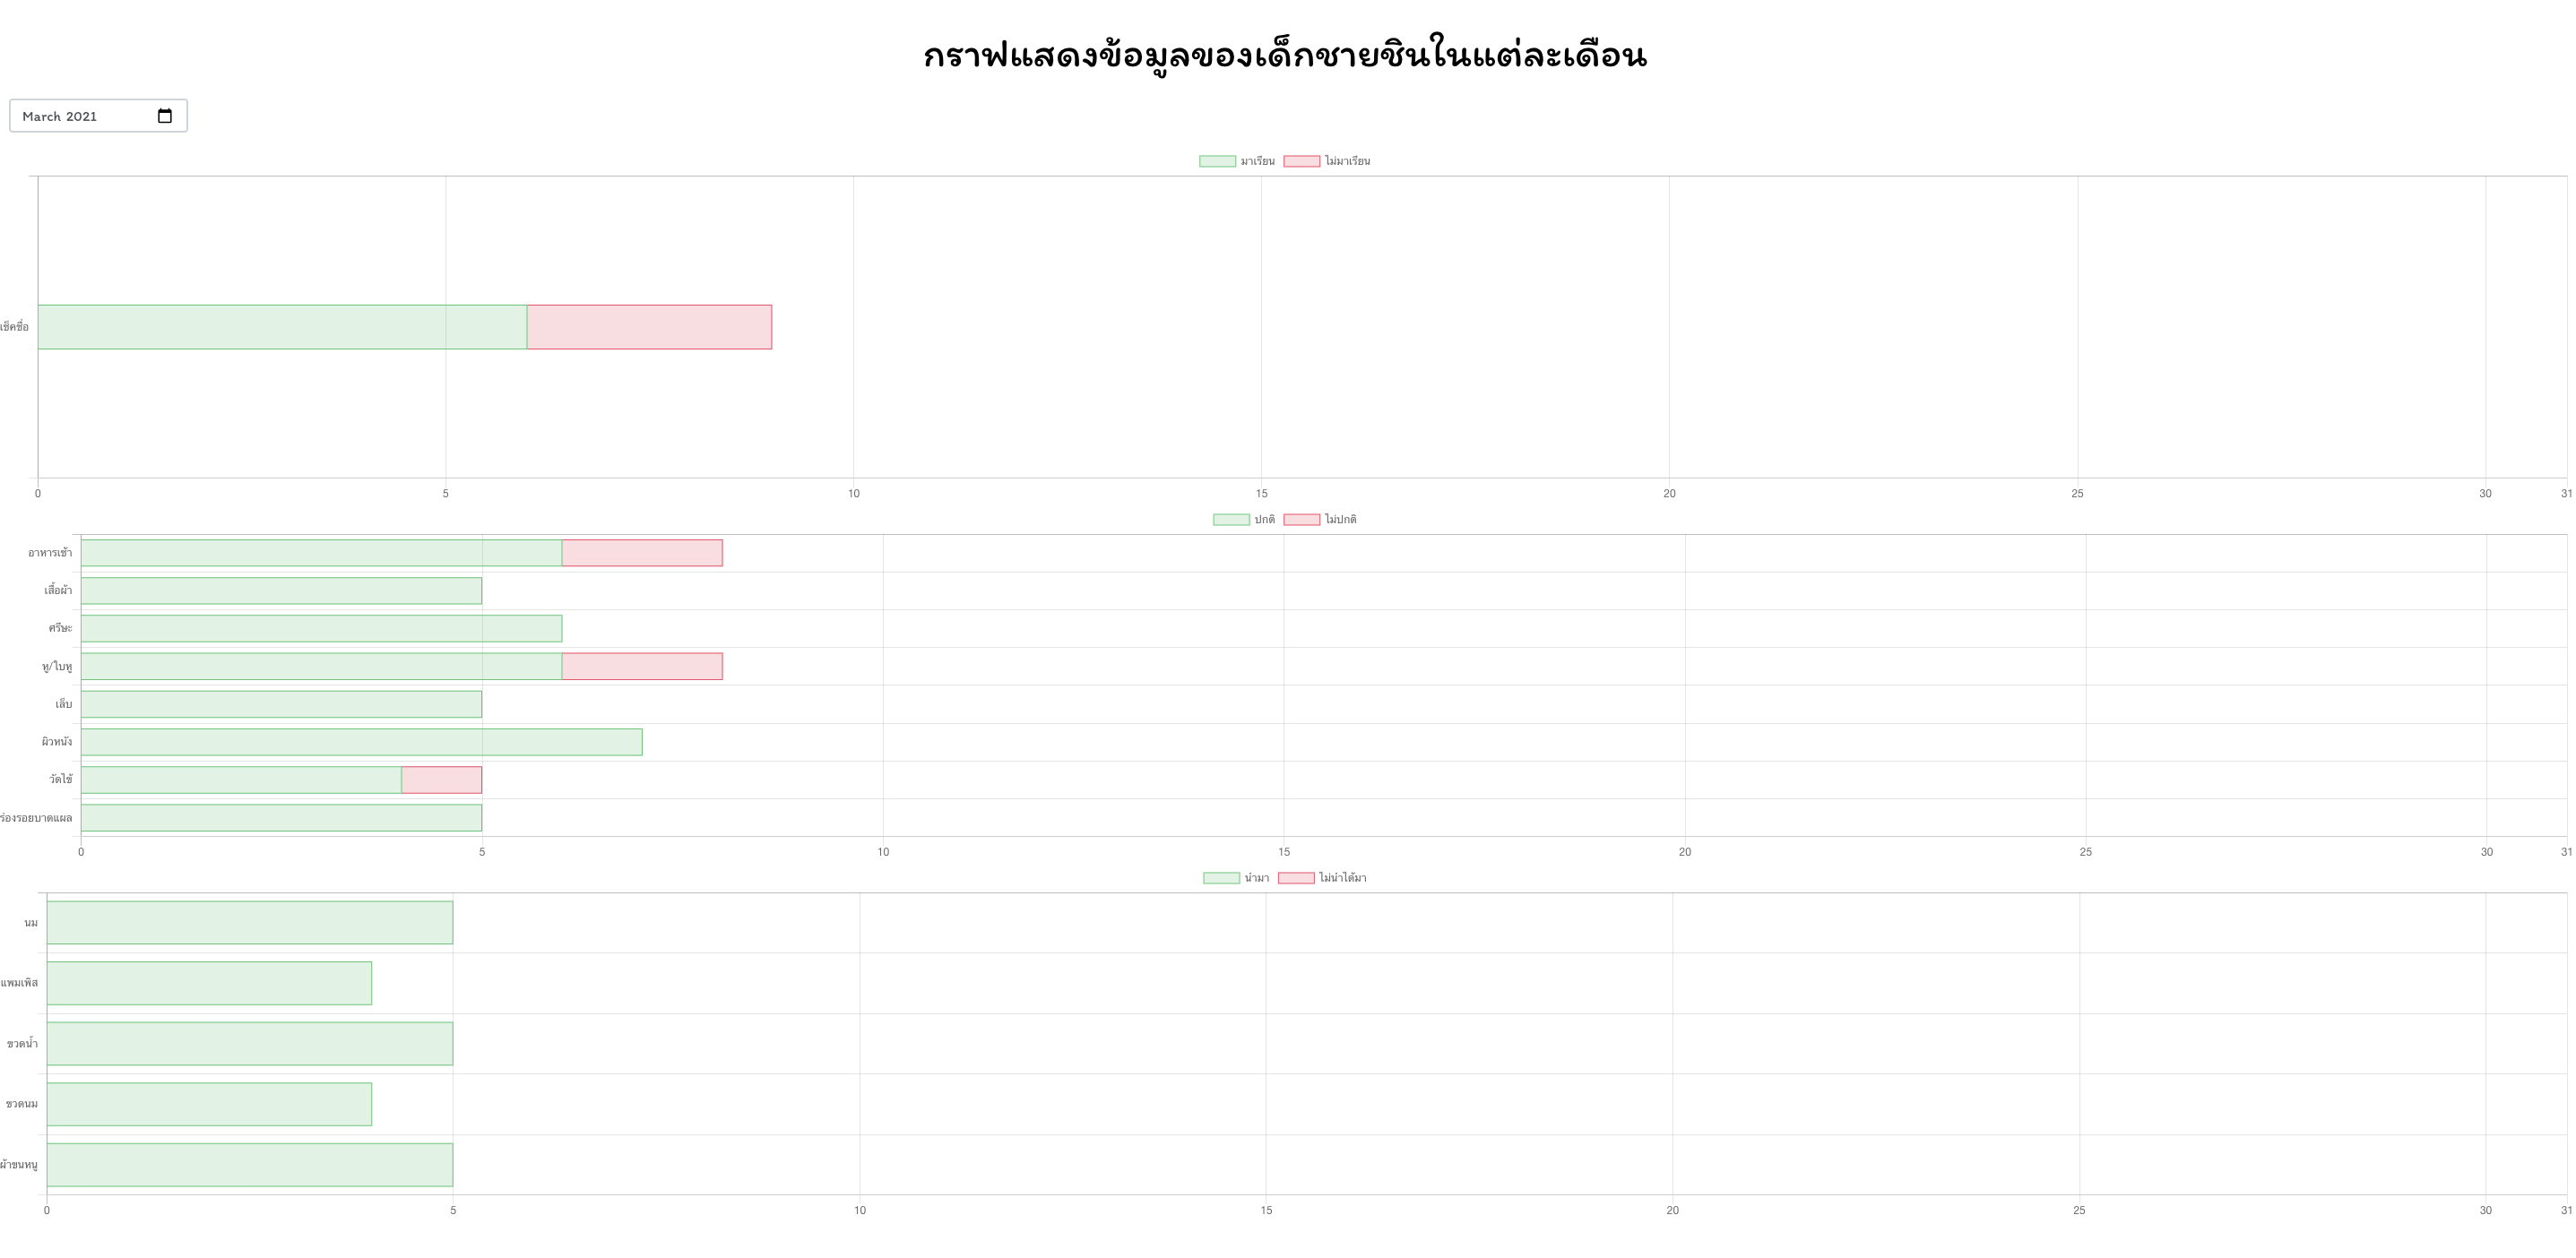
\includegraphics[width=\linewidth]{images/ChartPage.png}
    \end{center}
    \caption[หน้าแสดงข้อมูลรายเดือนเด็ก]{หน้าแสดงข้อมูลรายเดือนเด็ก}
    \label{fig:ChartPage}
  \end{figure}

  \begin{figure}
    \begin{center}
    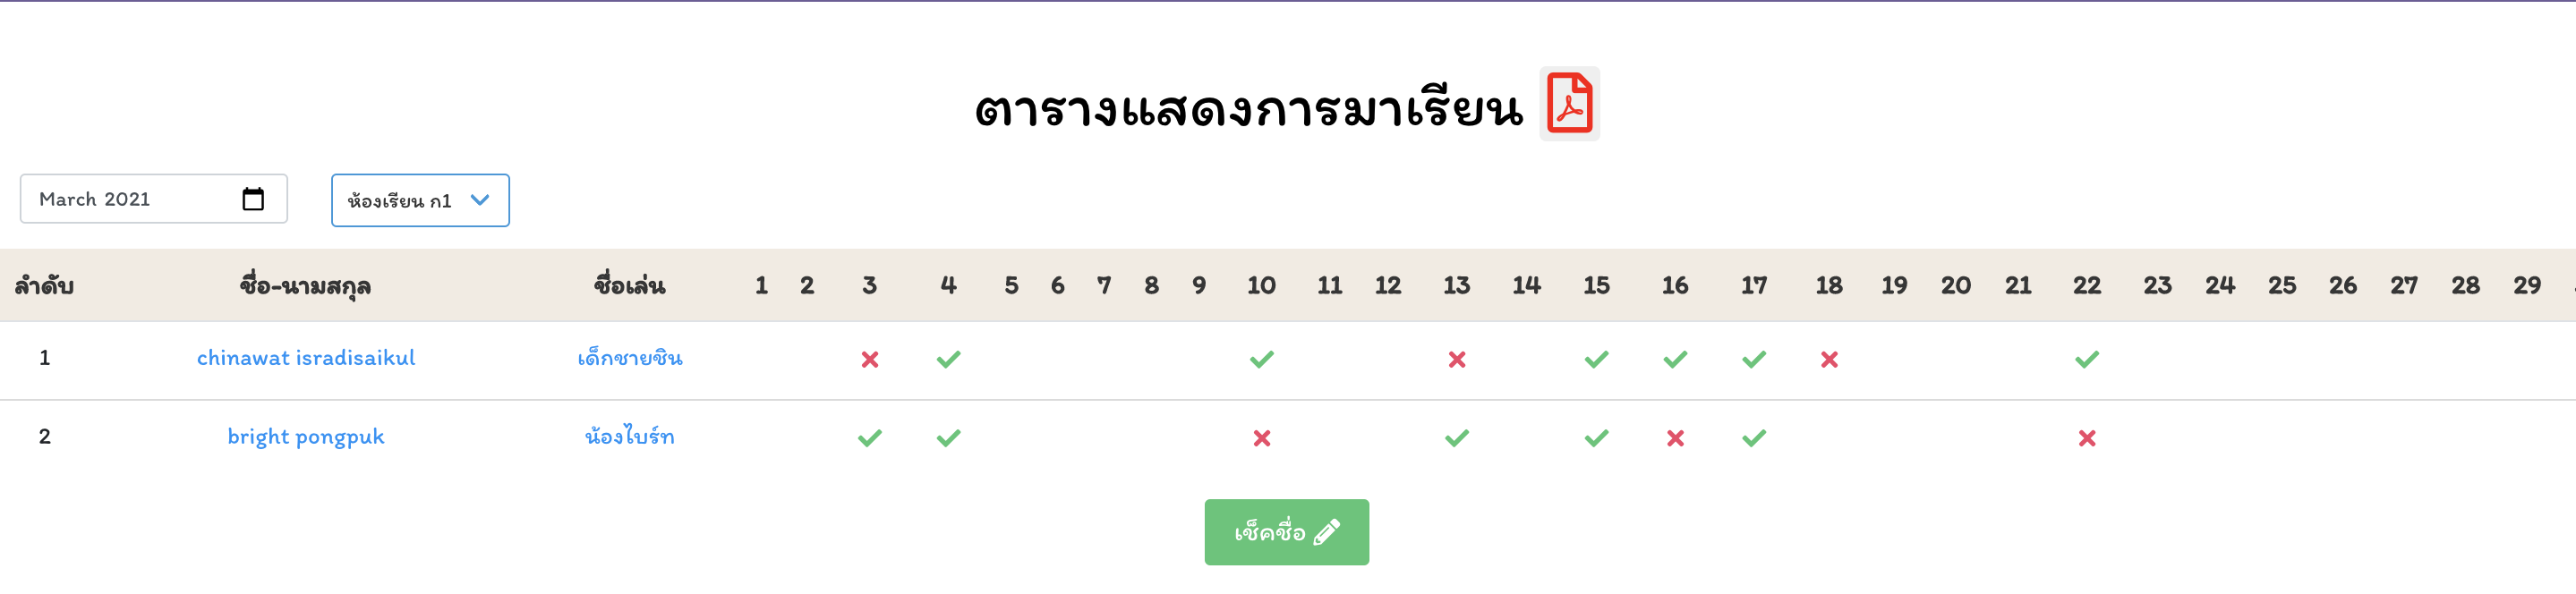
\includegraphics[width=\linewidth]{images/Attendance.png}
    \end{center}
    \caption[หน้าแสดงการเข้าเรียนเด็ก]{หน้าแสดงการเข้าเรียนเด็ก}
    \label{fig:Attendance}
  \end{figure}



  \begin{figure}
    \begin{center}
    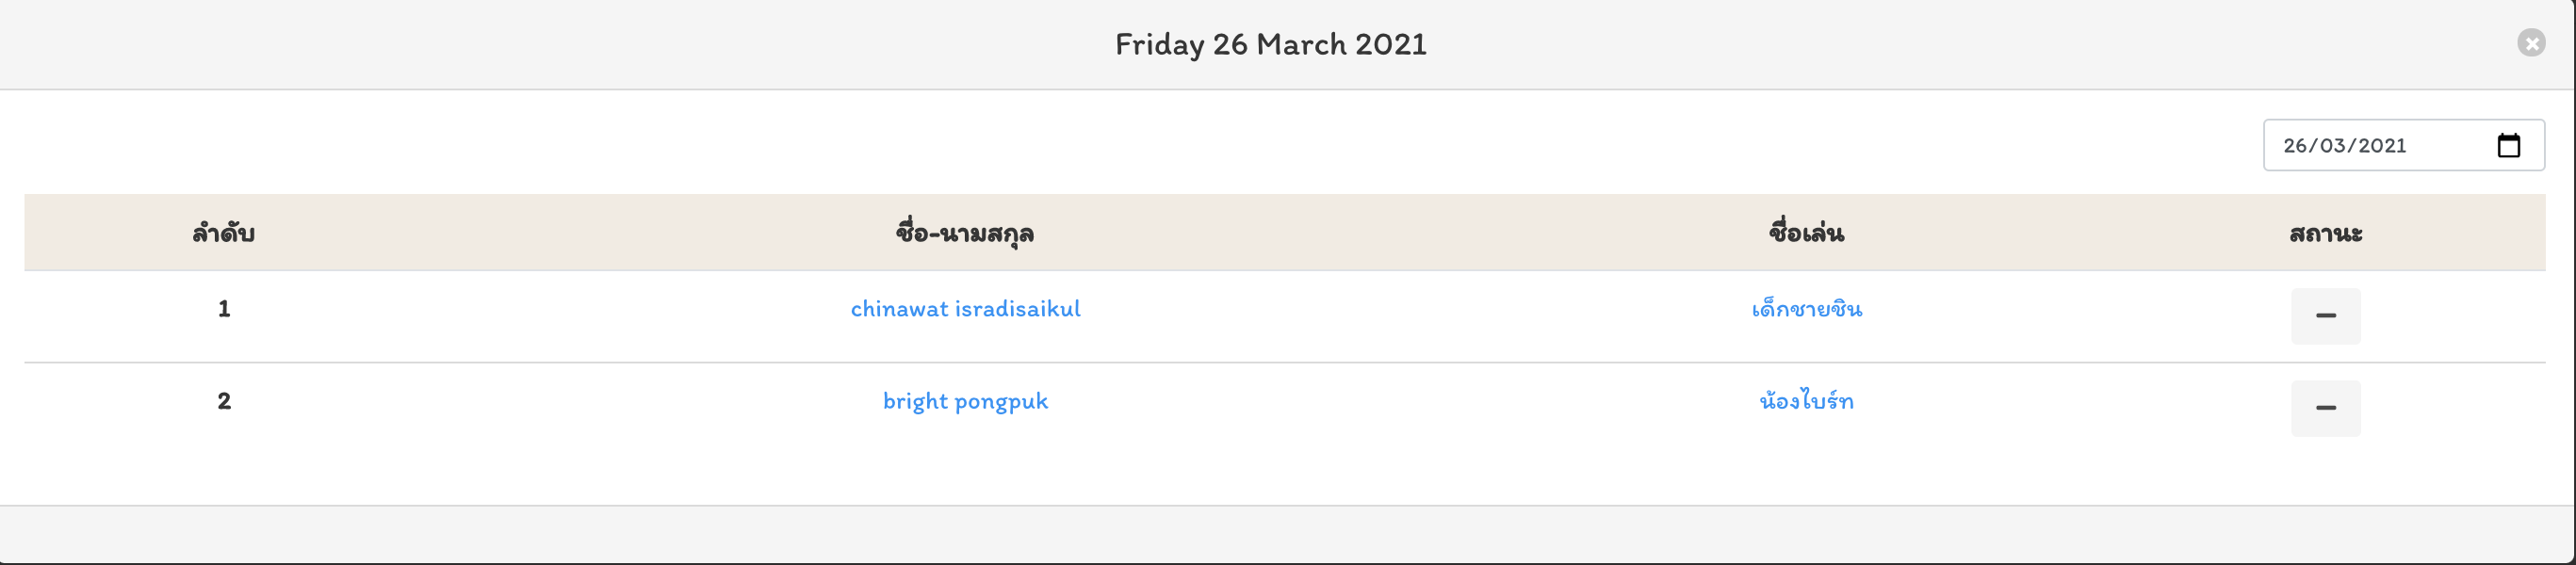
\includegraphics[width=\linewidth]{images/checkAttendance.png}
    \end{center}
    \caption[หน้าเช็คชื่อเด็ก]{หน้าเช็คชื่อเด็ก}
    \label{fig:CheckAttendance}
  \end{figure}

  \begin{figure}
    \begin{center}
    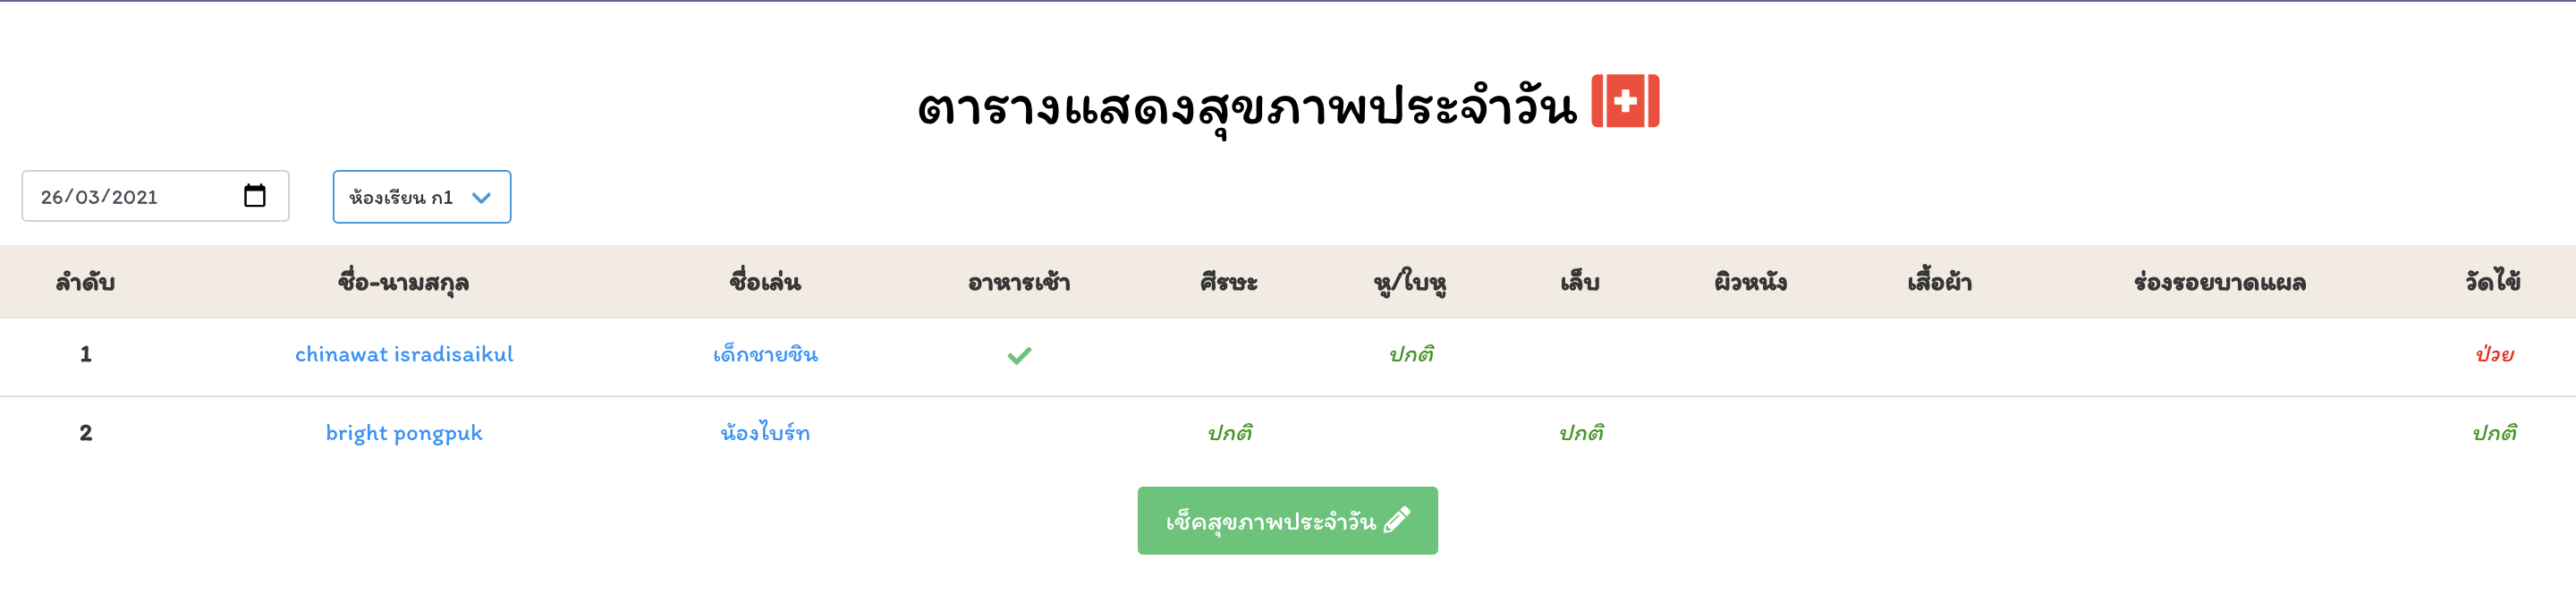
\includegraphics[width=\linewidth]{images/Health.png}
    \end{center}
    \caption[หน้าแสดงข้อมูลสุขภาพเด็กรายวัน]{หน้าแสดงข้อมูลสุขภาพเด็กรายวัน}
    \label{fig:Health}
    \end{figure}

  \begin{figure}
    \begin{center}
    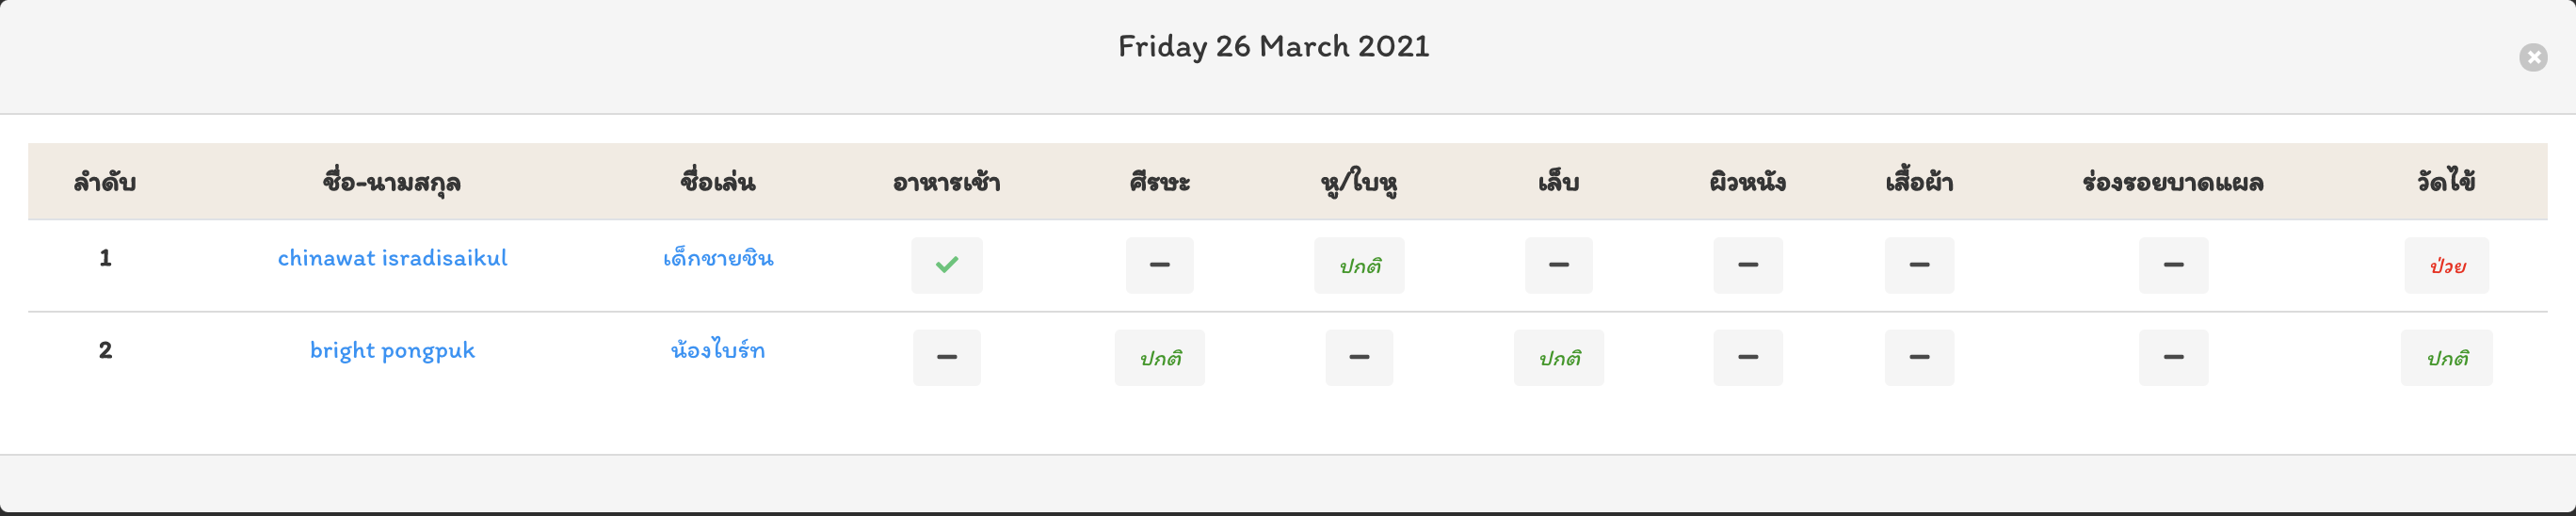
\includegraphics[width=\linewidth]{images/checkHealth.png}
    \end{center}
    \caption[หน้าเช็คสุขภาพเด็ก]{หน้าเช็คสุขภาพเด็ก}
    \label{fig:CheckHealth}
    \end{figure}

    \begin{figure}
      \begin{center}
      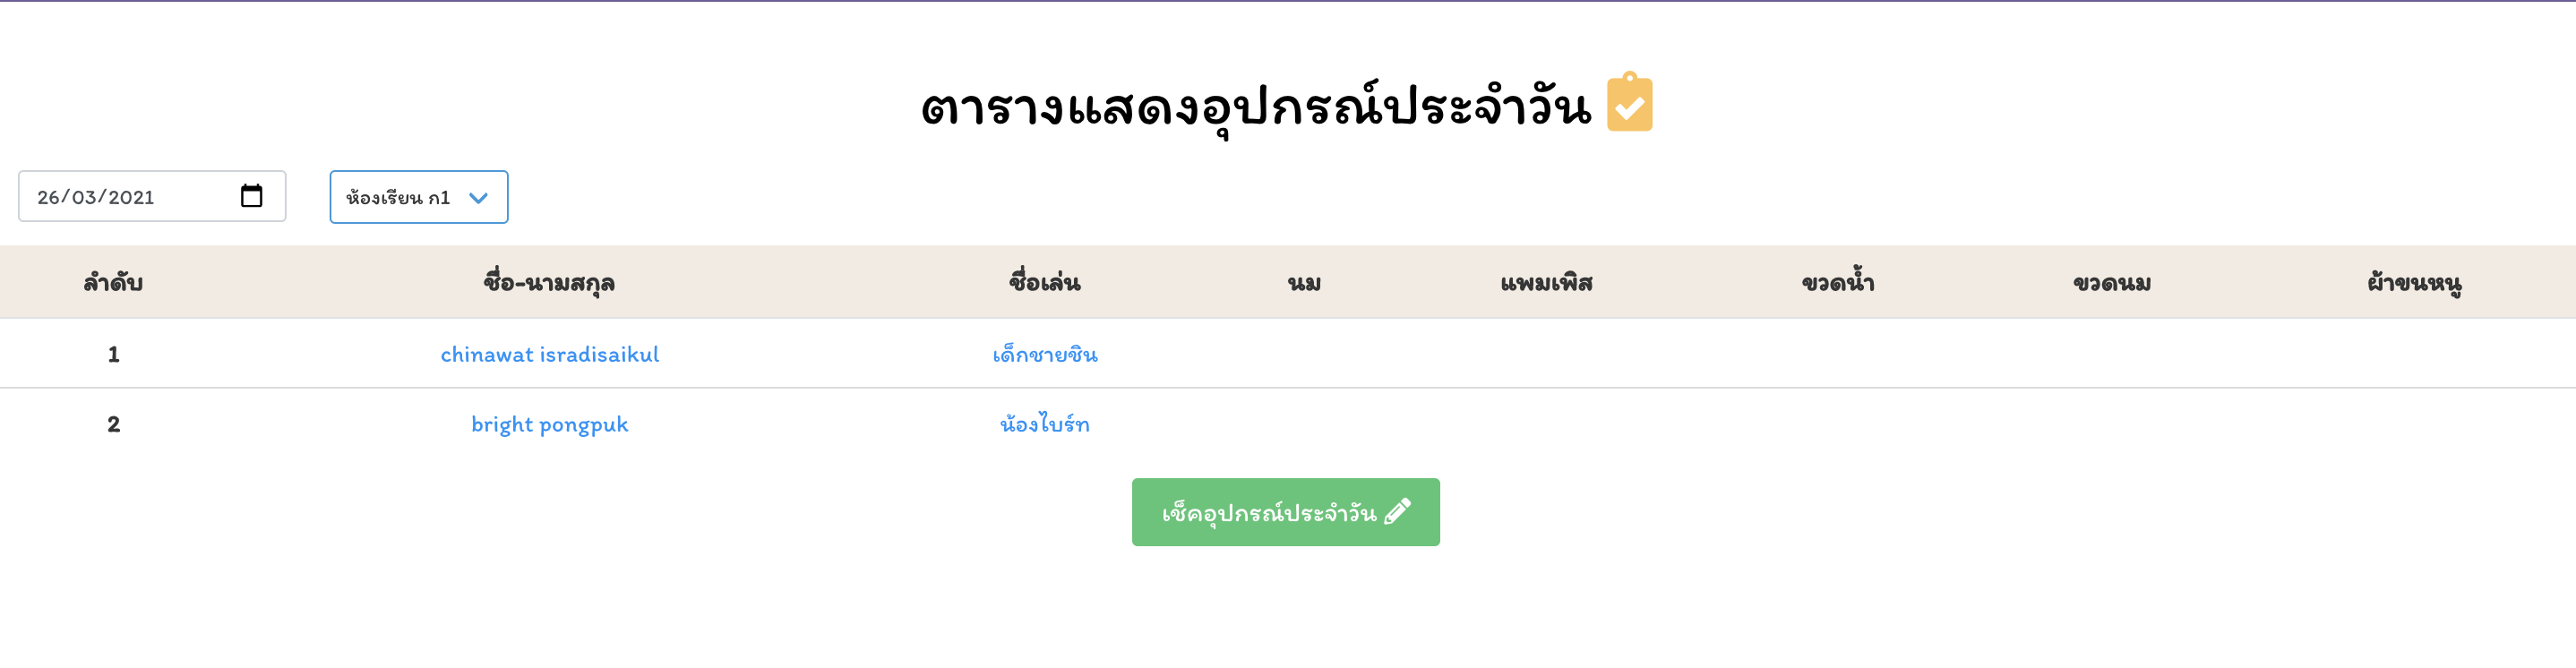
\includegraphics[width=\linewidth]{images/Gadget.png}
      \end{center}
      \caption[หน้าแสดงข้อมูลอุปกรณ์เด็กรายวัน]{หน้าแสดงข้อมูลอุปกรณ์เด็กรายวัน}
      \label{fig:Gadget}
      \end{figure}
  
    \begin{figure}
      \begin{center}
      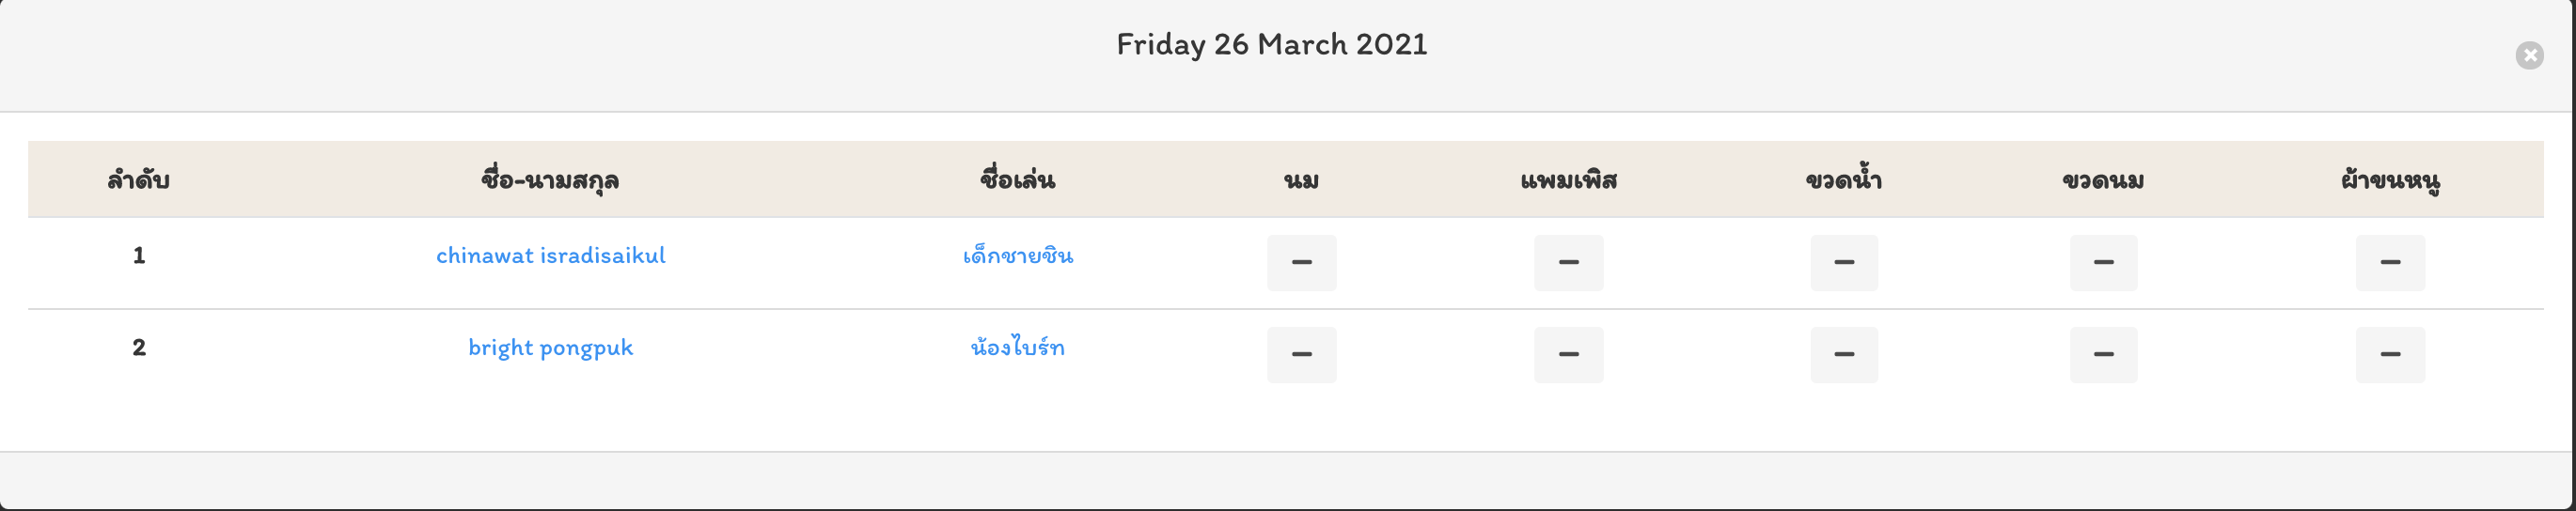
\includegraphics[width=\linewidth]{images/checkGadget.png}
      \end{center}
      \caption[หน้าเช็คอุปกรณ์เด็ก]{หน้าเช็คอุปกรณ์เด็ก}
      \label{fig:CheckGadget}
      \end{figure}
      \begin{figure}
        \begin{center}
        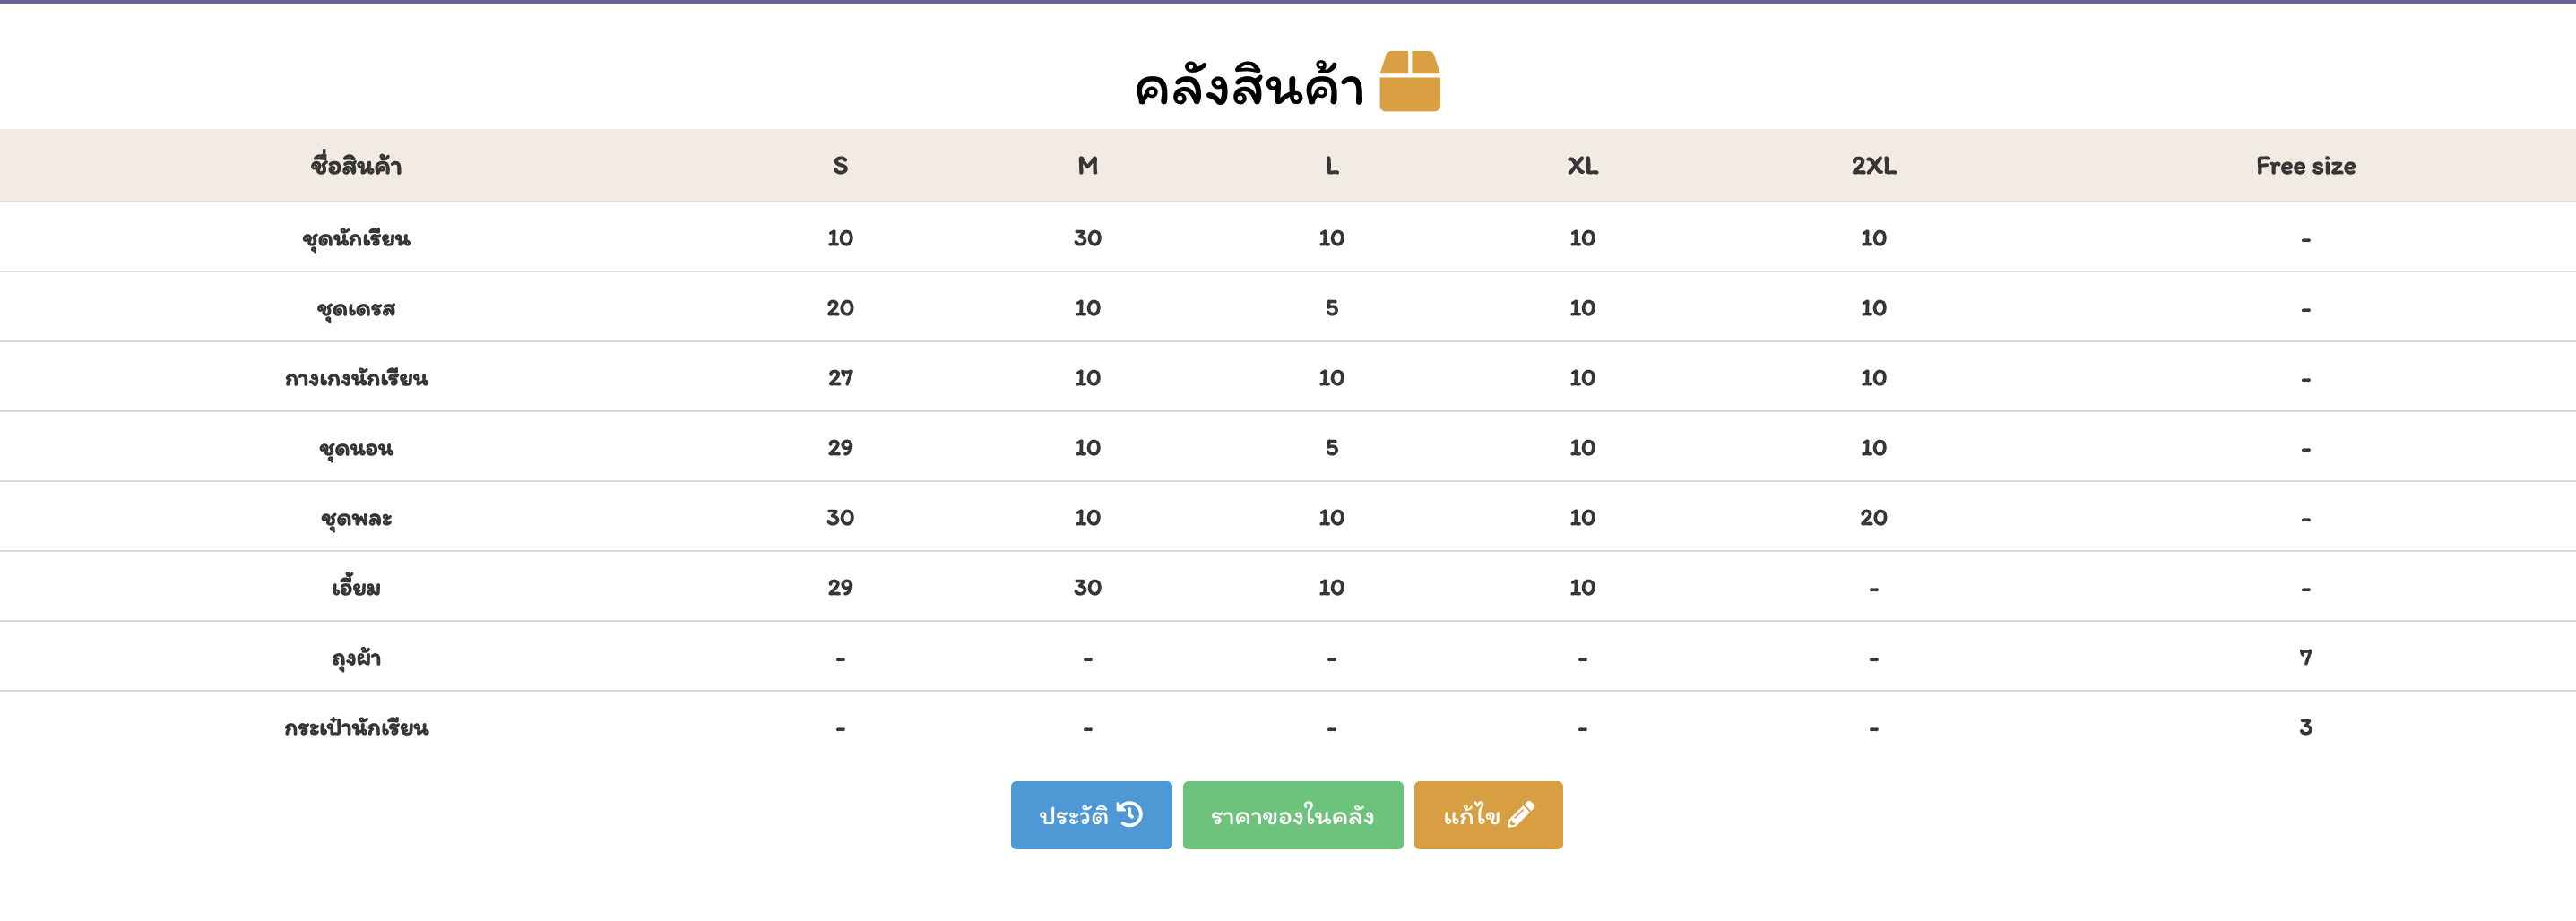
\includegraphics[width=\linewidth]{images/Stock.png}
        \end{center}
        \caption[หน้าแสดงคลังสินค้า]{หน้าแสดงคลังสินค้า}
        \label{fig:Stock}
        \end{figure}
    
    
      \begin{figure}
        \begin{center}
        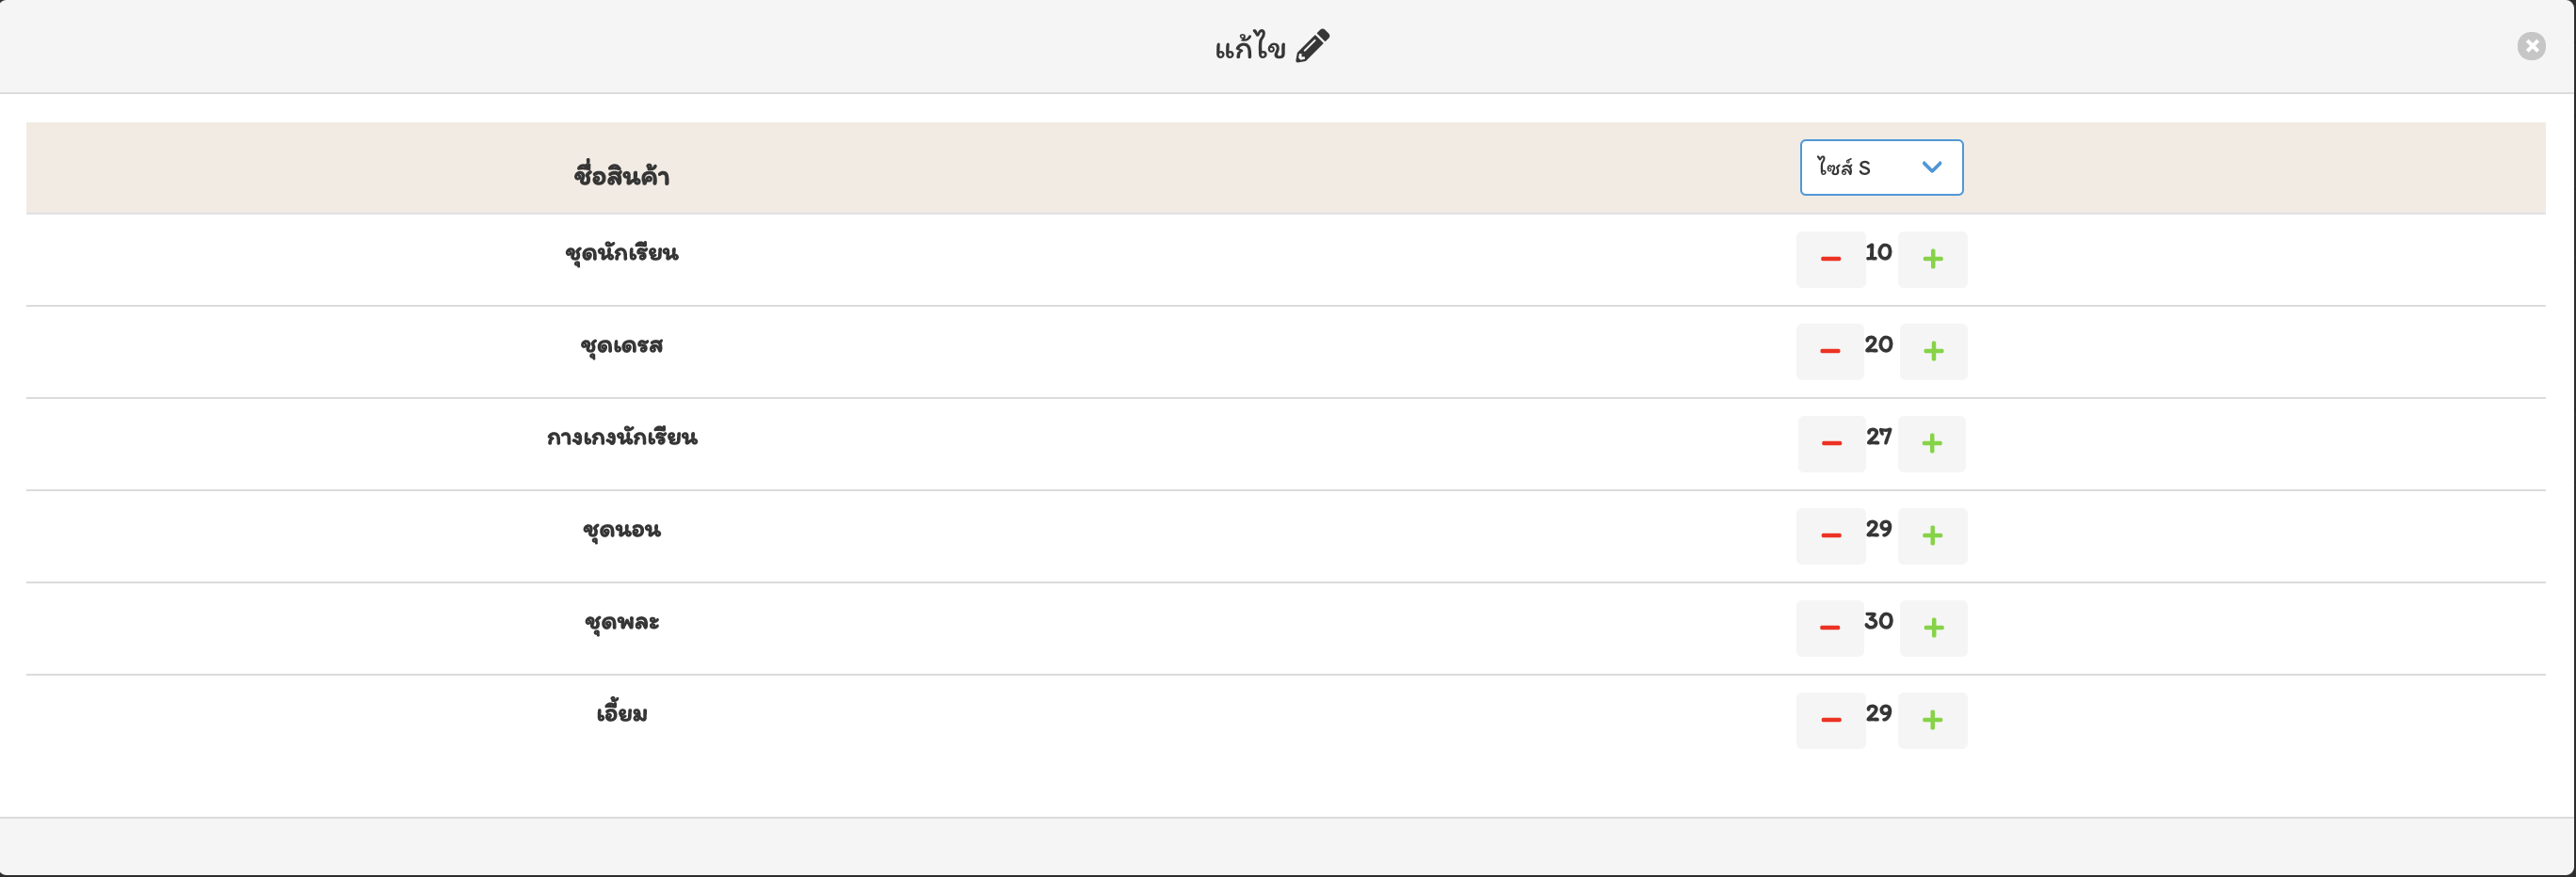
\includegraphics[width=\linewidth]{images/handleStock.png}
        \end{center}
        \caption[หน้าจัดการแก้ไขสต็อกของ]{หน้าจัดการแก้ไขสต็อกของ}
        \label{fig:CheckStock}
        \end{figure}
    
    
    
      \begin{figure}
        \begin{center}
        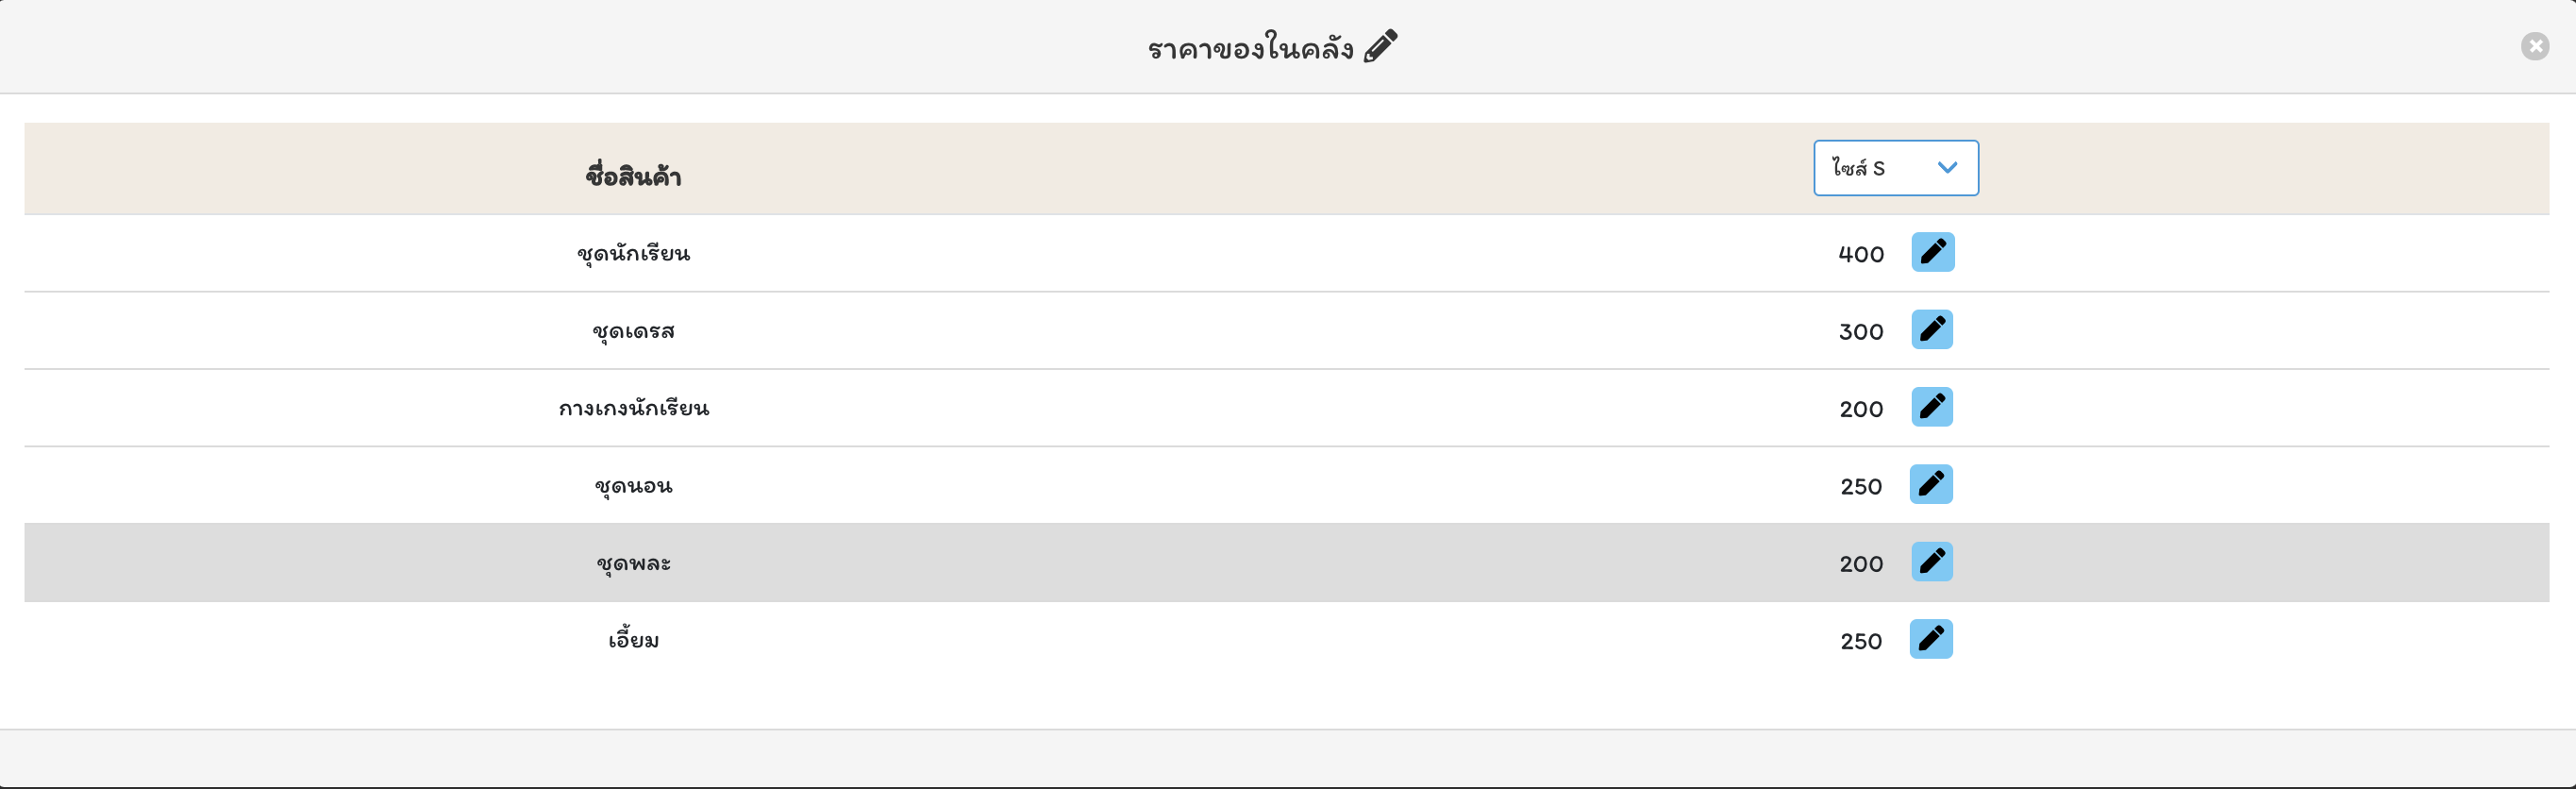
\includegraphics[width=\linewidth]{images/editPrice.png}
        \end{center}
        \caption[หน้าจัดการแก้ไขราคาสินค้า]{หน้าจัดการแก้ไขราคาสินค้า}
        \label{fig:editPrice}
        \end{figure}
    
    
      \begin{figure}
        \begin{center}
        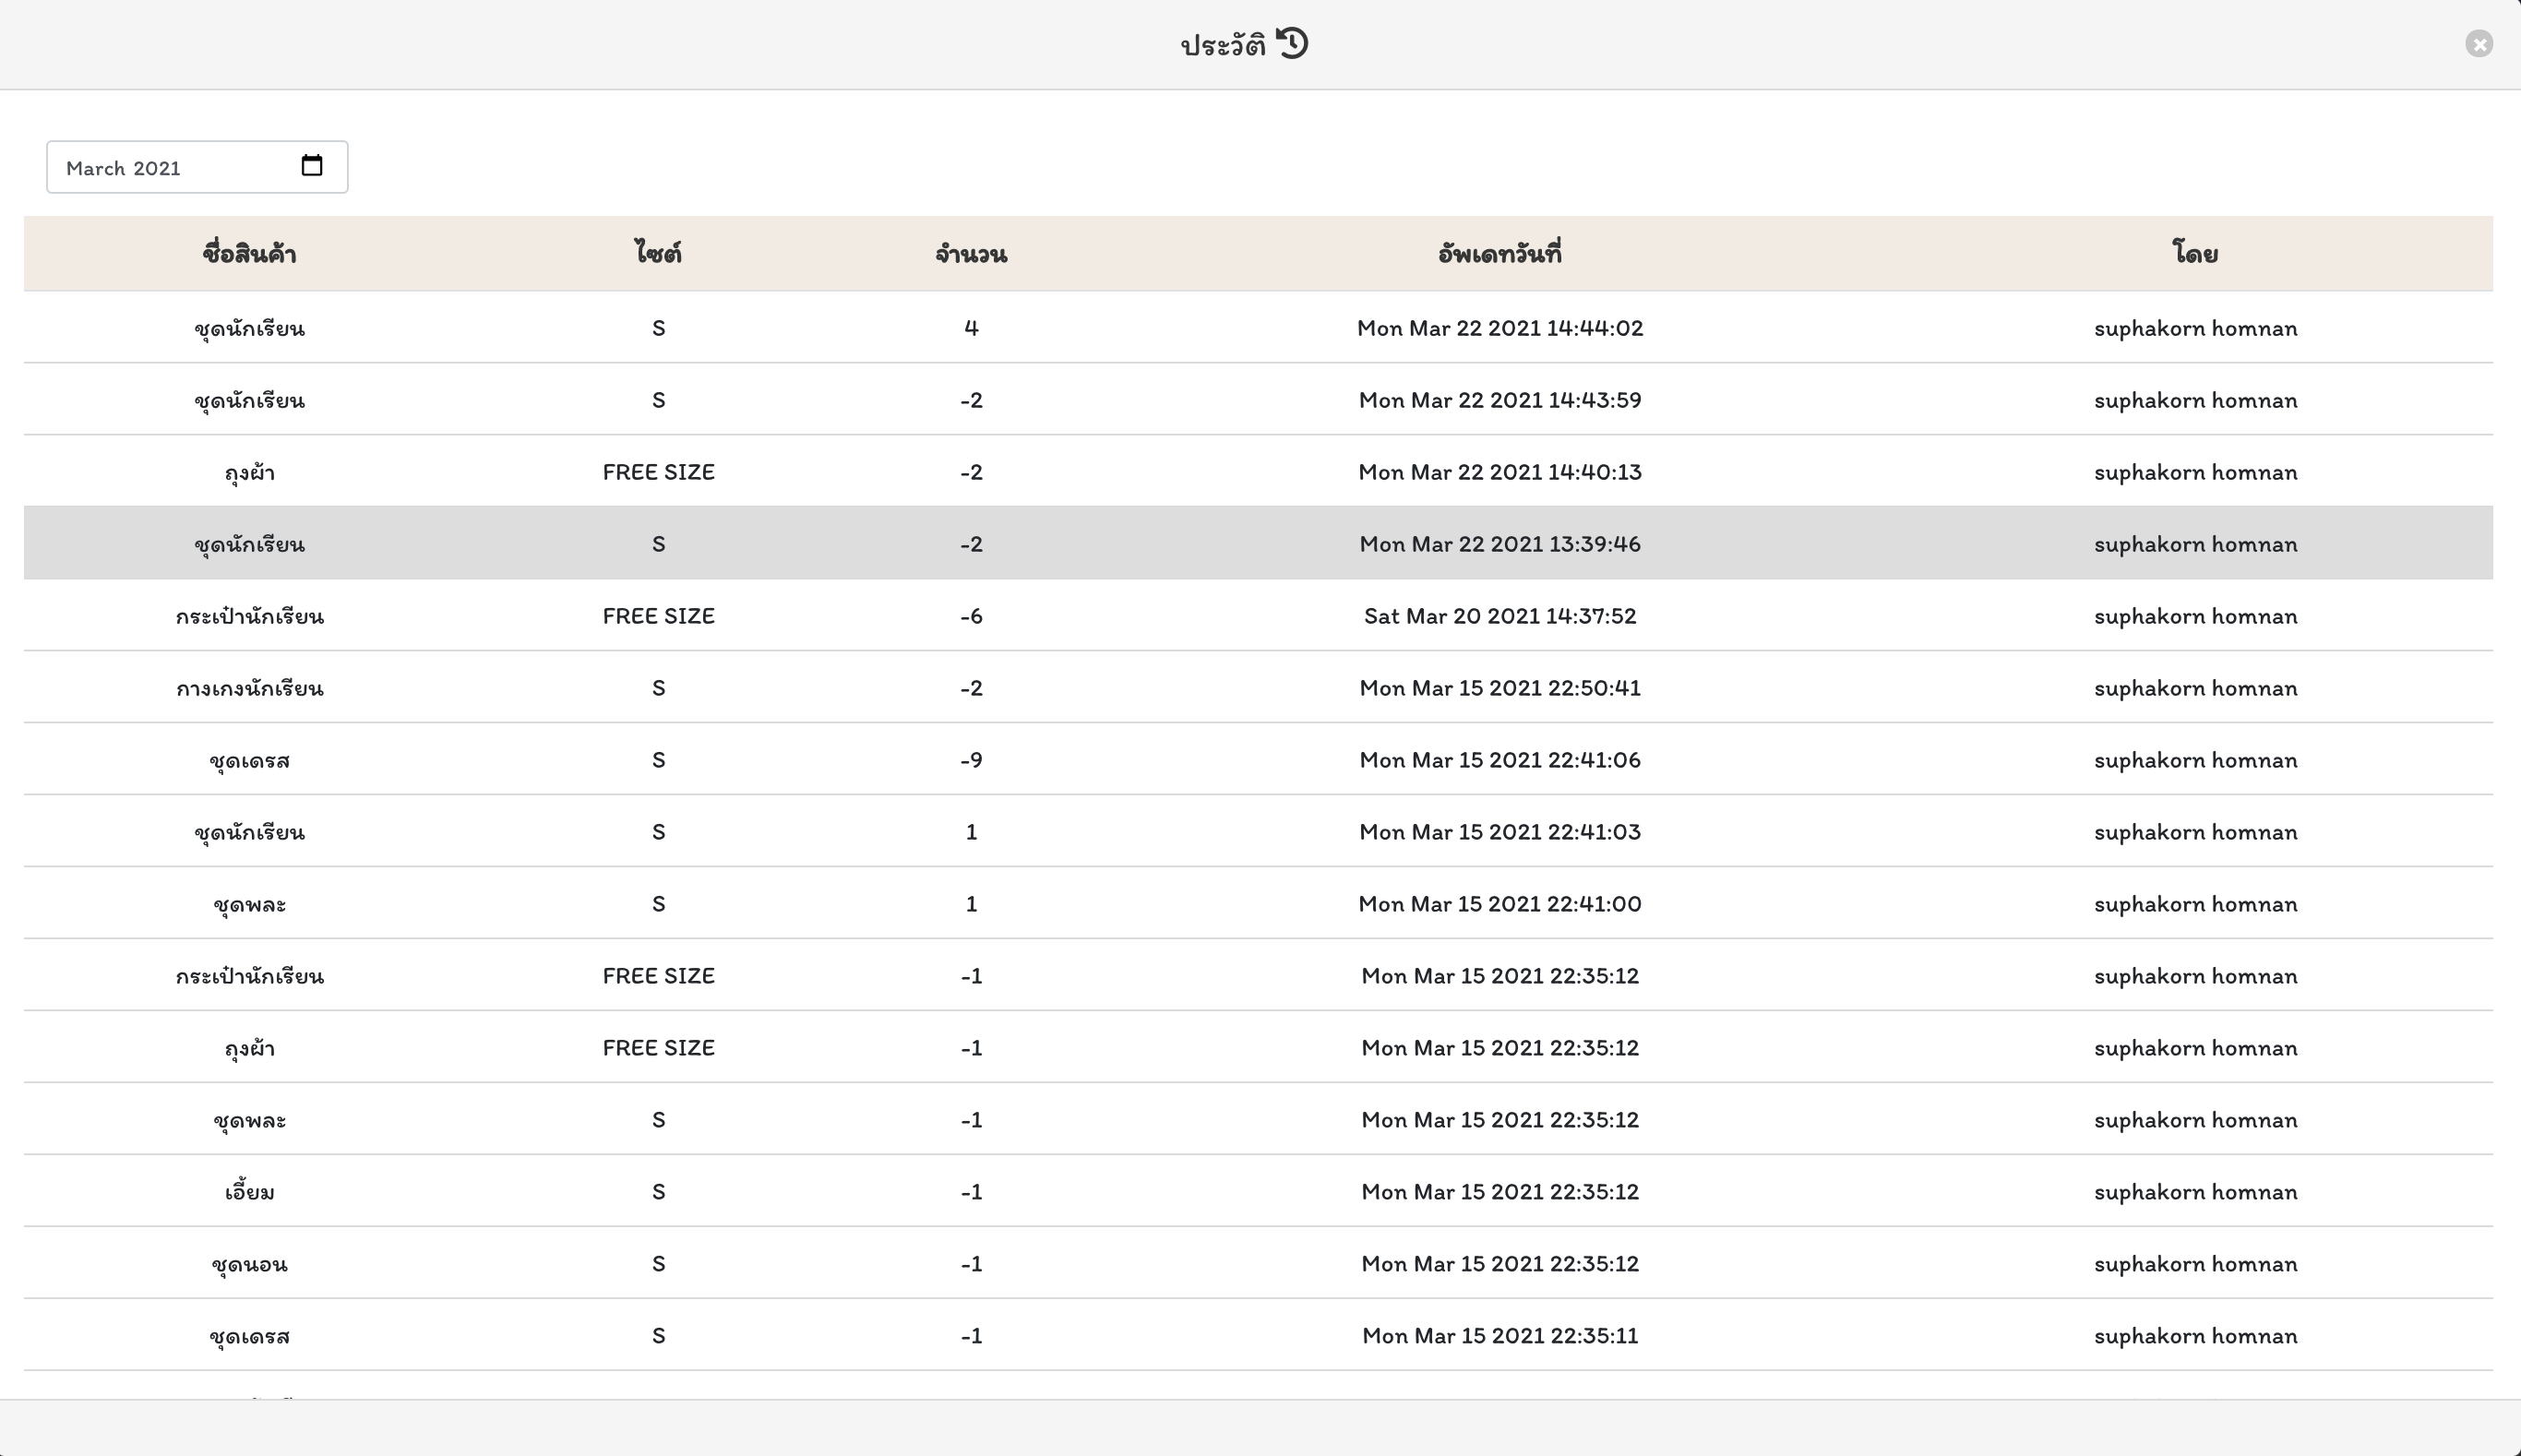
\includegraphics[width=\linewidth]{images/historyStock.png}
        \end{center}
        \caption[หน้าแสดงประวัติการเพิ่มลดของ]{หน้าแสดงประวัติการเพิ่มลดของ}
        \label{fig:HistoryStock}
      \end{figure}
      \begin{figure}
        \begin{center}
        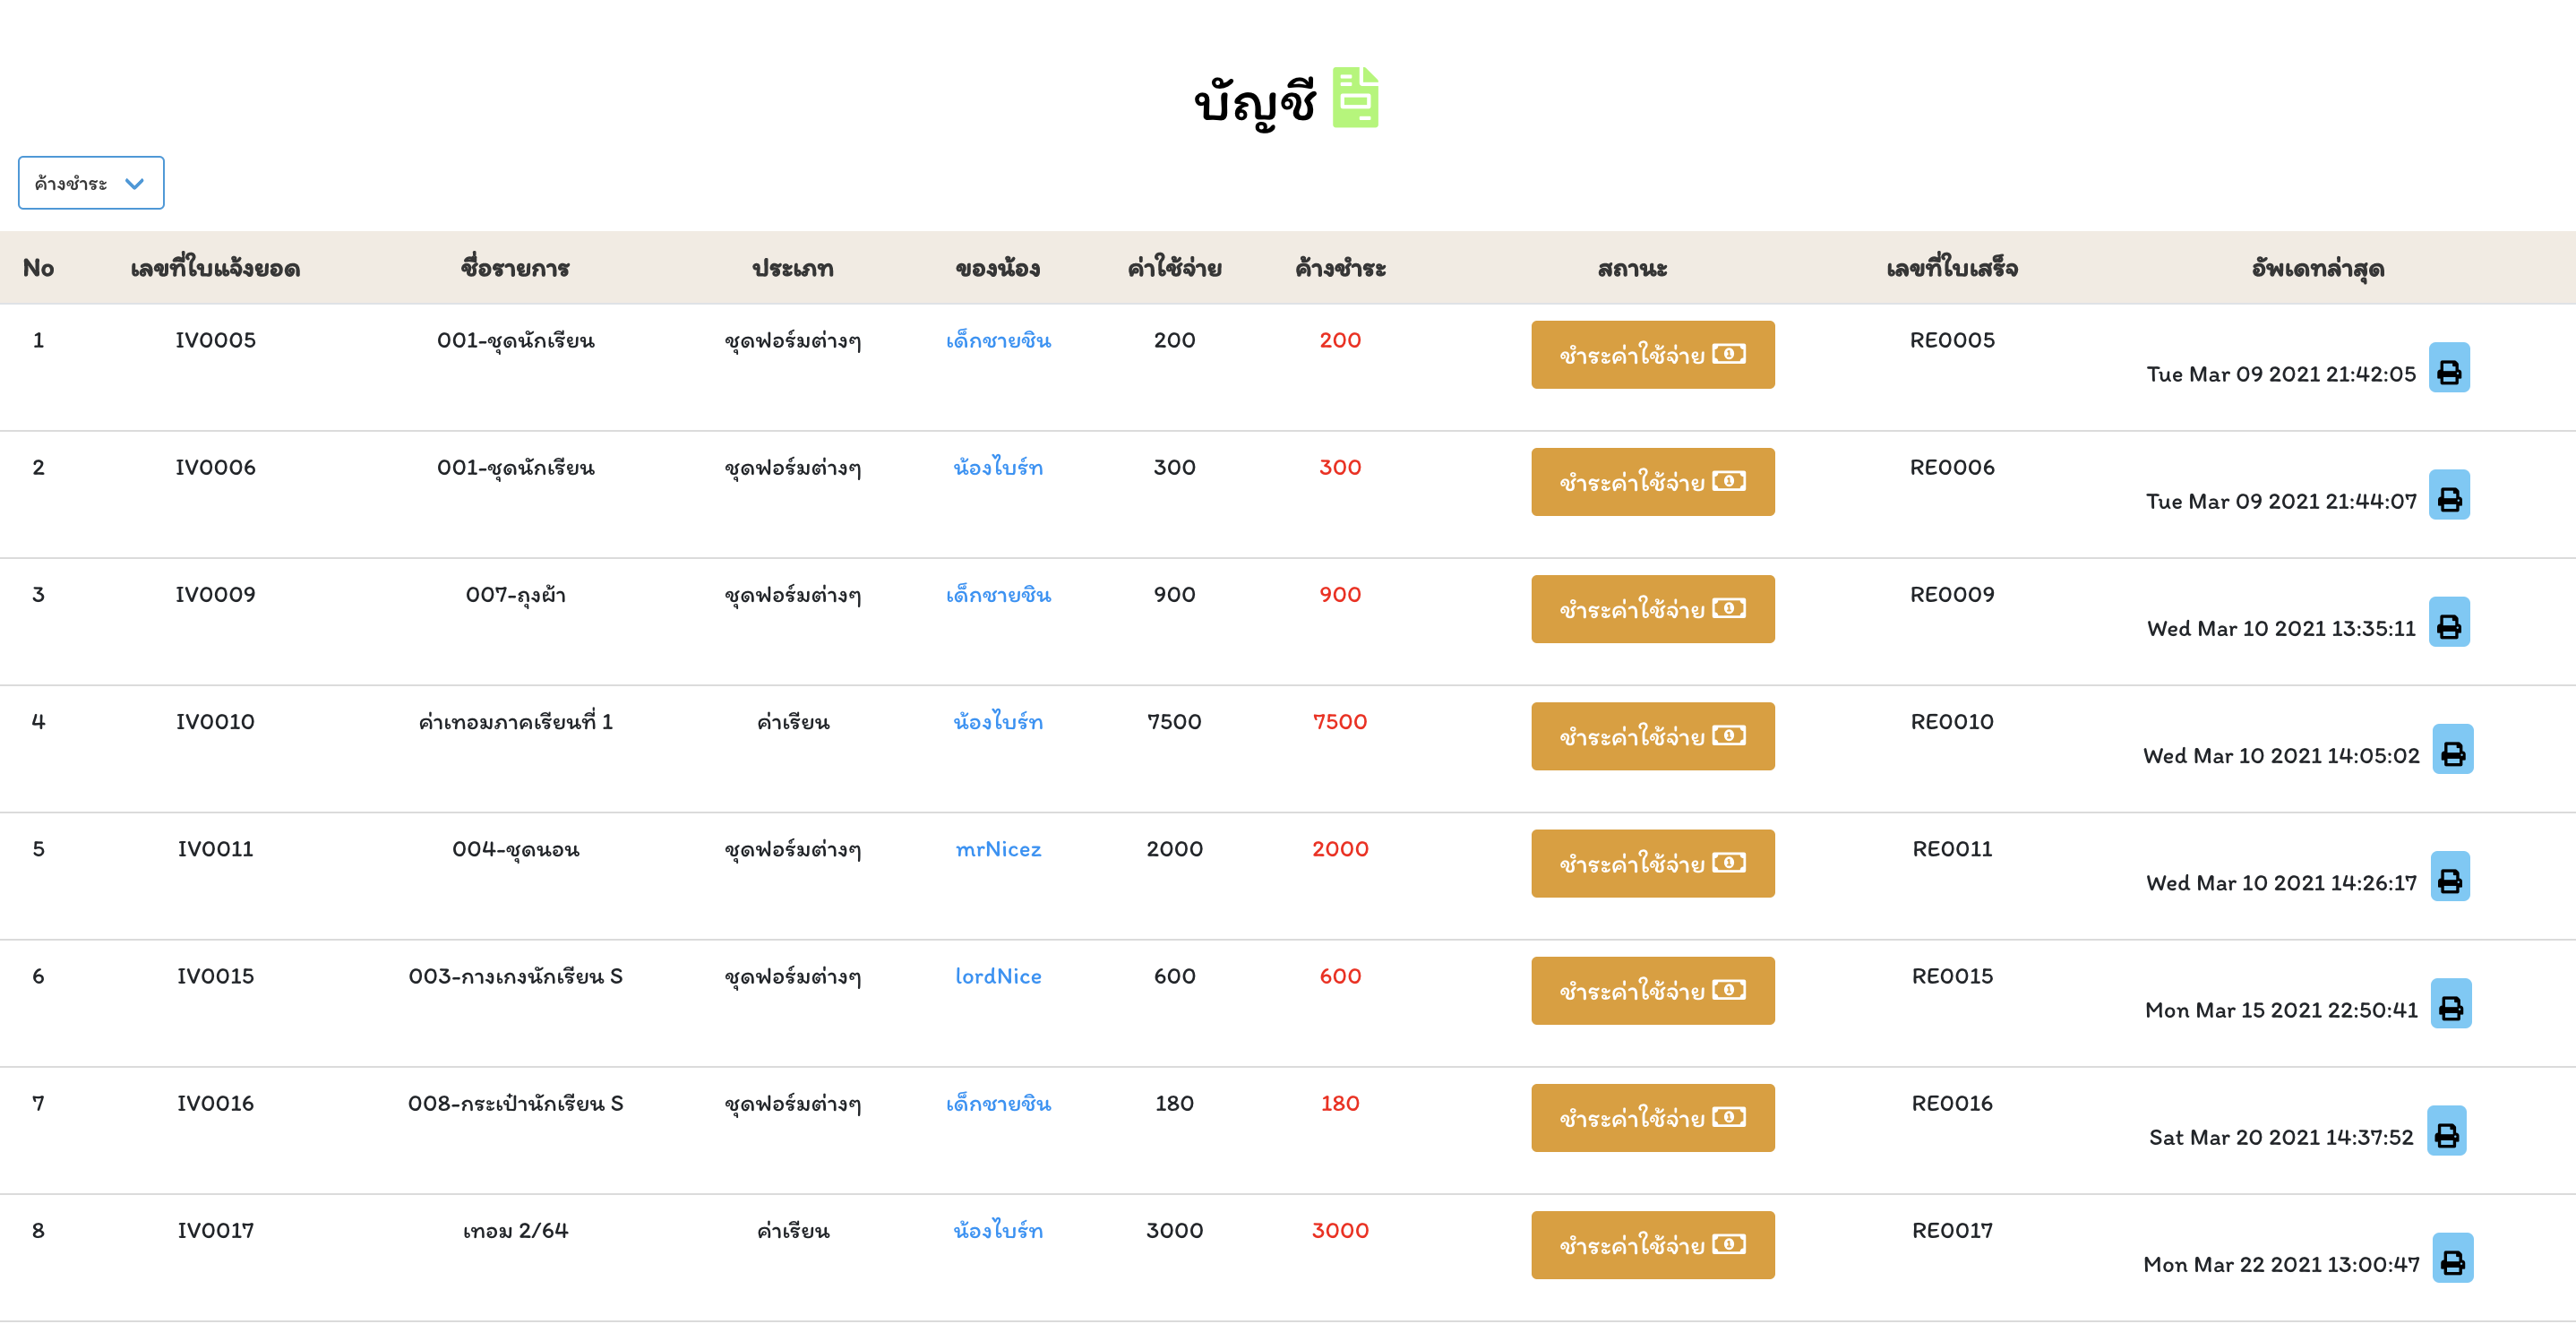
\includegraphics[width=\linewidth]{images/Payment.png}
        \end{center}
        \caption[หน้าแสดงรายการบัญชี]{หน้าแสดงรายการบัญชี}
        \label{fig:Payment}
      
        \end{figure}
    
      \begin{figure}
        \begin{center}
        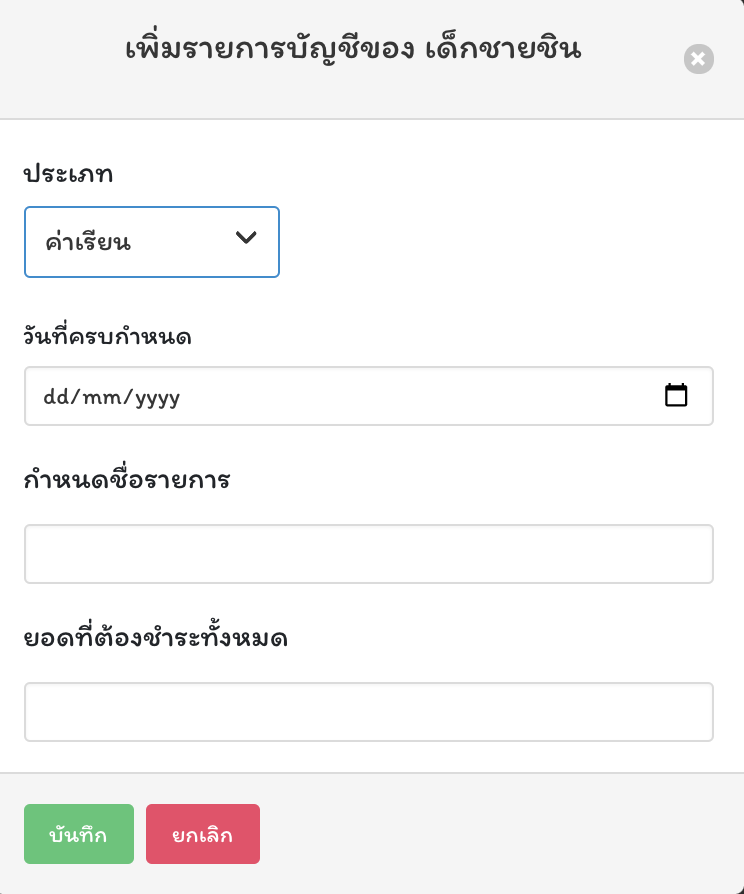
\includegraphics[scale=0.5]{images/CreatePayment.png}
        \end{center}
        \caption[หน้าเพิ่มรายการบัญชี]{หน้าเพิ่มรายการบัญชี}
        \label{fig:CreatePayment}
        \end{figure}
    
    
      \begin{figure}
        \begin{center}
        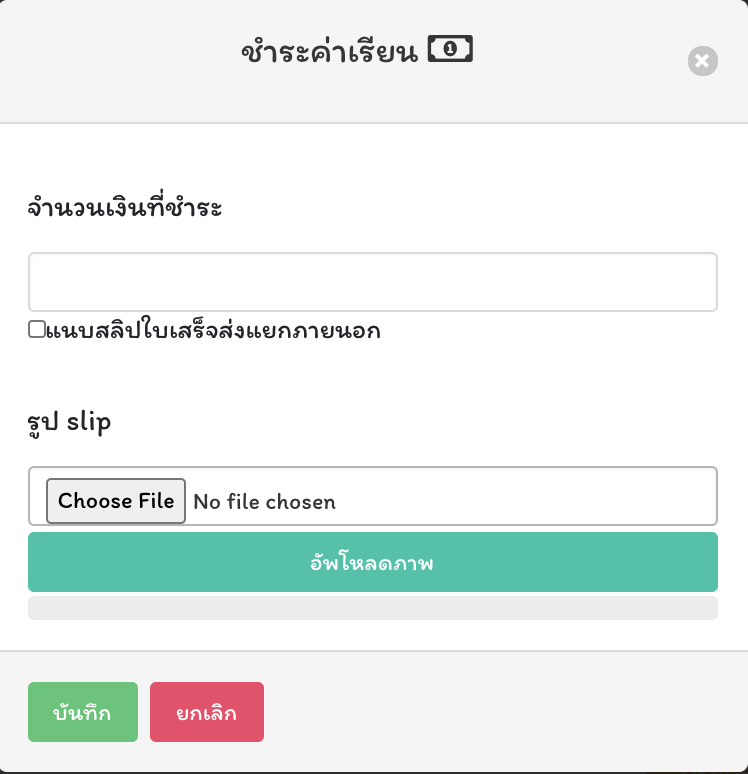
\includegraphics[scale=0.5]{images/UpdatePayment.png}
        \end{center}
        \caption[หน้าชำระค่าใช้จ่าย]{หน้าชำระค่าใช้จ่าย}
        \label{fig:updatePayment}
        \end{figure}
    
        \begin{figure}
          \begin{center}
          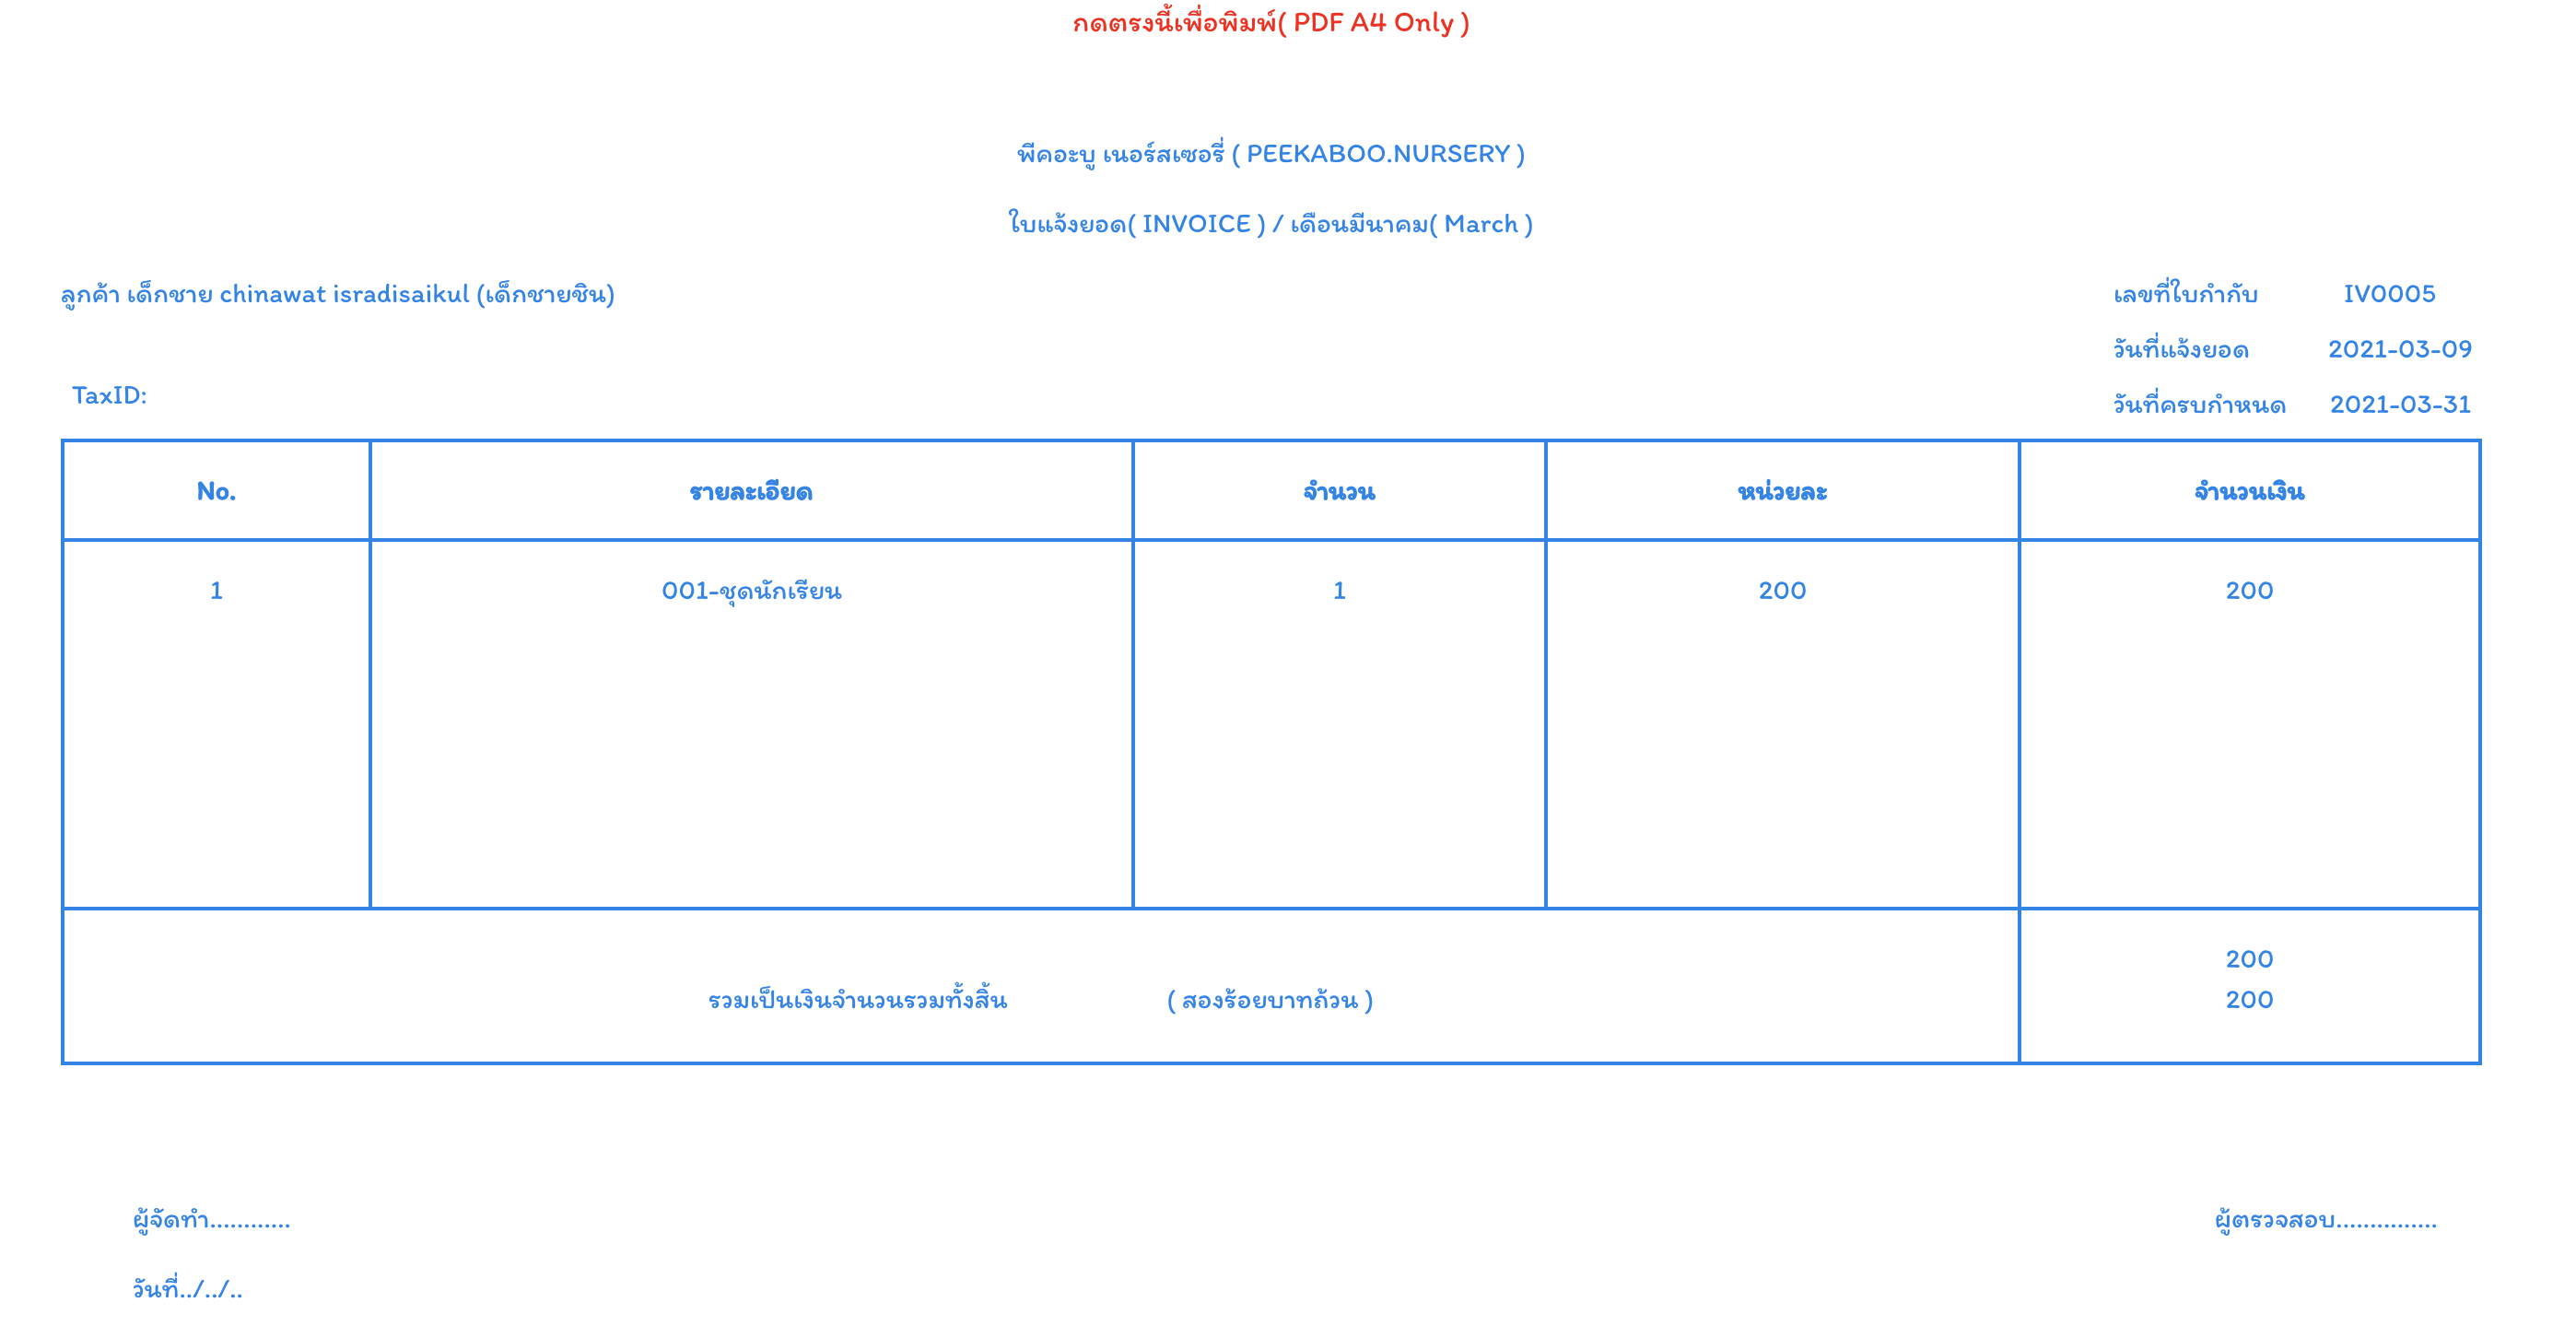
\includegraphics[width=\linewidth]{images/invoicePage.png}
          \end{center}
          \caption[หน้าปริ้นใบแจ้งยอด]{หน้าปริ้นใบแจ้งยอด}
          \label{fig:invoicePage}
          \end{figure}
    
        \begin{figure}
          \begin{center}
          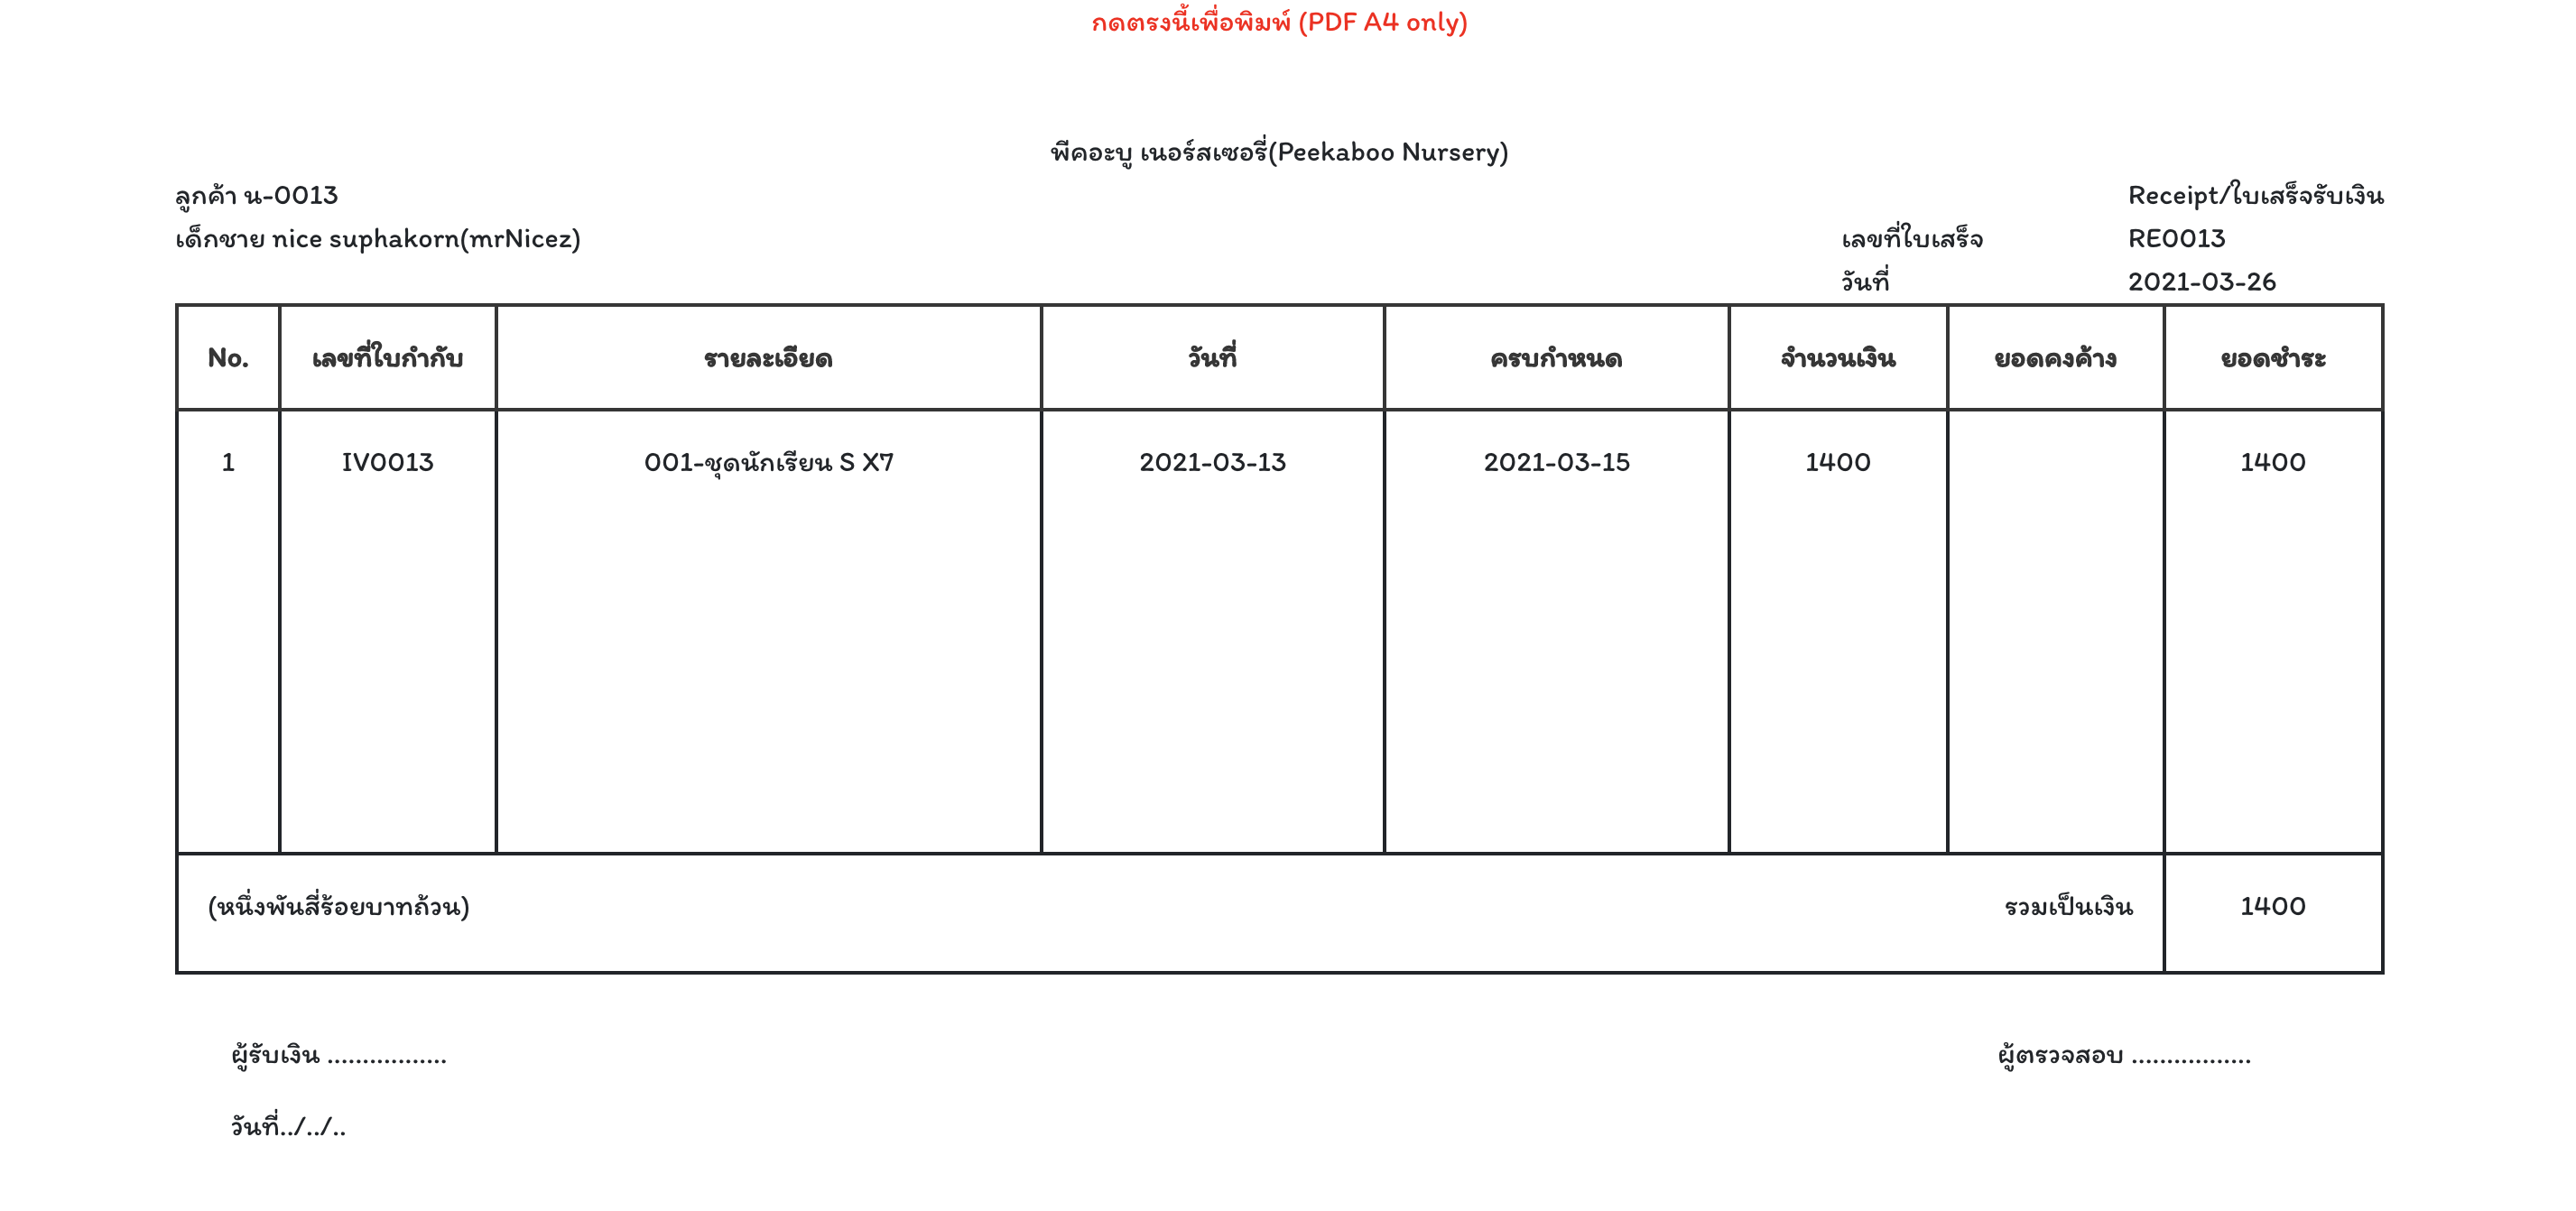
\includegraphics[width=\linewidth]{images/slipPage.png}
          \end{center}
          \caption[หน้าปริ้นใบเสร็จ]{หน้าปริ้นใบเสร็จ}
          \label{fig:slipPage}
          \end{figure}

\chapter{\ifproject%
\ifcpe การทดลองและผลลัพธ์\else Experimentation and Results\fi
\else%
\ifcpe การประเมินระบบ\else System Evaluation\fi
\fi}


\section{ระบบต้องทำงานได้ทั้งหมดดังนี้}
\paragraph{การกรอกใบสมัคร}
\begin{itemize}
    \item การกรอกใบสมัครจะต้องครบถ้วนสมบูรณ์ตามเงื่อนไขที่กำหนดไว้
    \begin{itemize}
        \item วิธีการทดสอบคือ ต้องกรอกชื่อจริง ชื่อเล่น วันเดือนปีเกิด ไม่เช่นนั้น จะไม่สามารถดำเนินการต่อไปในขั้นตอนถัดไปได้ จำเป็นต้องกรอกให้ครบถ้วนก่อนเสมอ
    \end{itemize}
\end{itemize}
\paragraph{การเช็คชื่อ}
\begin{itemize}
    \item ต้องสามารถเช็คชื่อในแต่ละวันและเช็คชื่อย้อนหลังได้
    \begin{itemize}
        \item ขั้นตอนการทดสอบการเช็คชื่อคือ เช็คชื่อเด็กในแต่ละวัน  ถ้าเช็คว่ามาก็จะมีสัญลักษณ์เช็คถูกขึ้นมาใน column ของวันที่เช็ค ในแถวของเด็กคนนั้น  หากเด็กคนนั้นไม่มา ก็จะมีสัญลักษณ์ขีดแดทขึ้นบนช่องนั้น
        \item ขั้นตอนการทดสอบการเช็คชื่อย้อนหลังคือ  เมื่อต้องการแก้ไขให้เด็กคนหนึ่งที่มาเรียนสายมากๆ  จนทำให้คุณครูลืมเช็คชื่อ  จึงต้องทำการเช็คชื่อย้อนหลังในวันถัดๆไป  เพื่อแก้ไขให้เด็กที่มาสายคนนั้นในหน้าแสดงผลให้สัญลักษณ์ขีดแดท กลายเป็น สัญลักษณ์เช็คถูก  โดยจะตรวจสอบด้วยการเลือกวันที่ต้องการเช็คย้อนหลังแล้วทำการเช็คชื่อ  ถ้าหากระบบทำงานได้ปกติ  จะต้องได้ผลลัพธ์แบบที่กล่าวไว้ข้างต้น
    \end{itemize}
\end{itemize}
\paragraph{การตรวจสุภาพประจำวัน}
\begin{itemize}
    \item สามารถเช็คสุขภาพประจำวันได้ครบถ้วนตามที่ระบุไว้และสามารถเช็คย้อนหลังได้
    \begin{itemize}
        \item ขั้นตอนการทดสอบคือ เมื่อมีการเช็คของ ของเด็กแต่ละคน  เมื่อเช็คว่าเอามาใน column ของวันที่เช็ค ในแถวของเด็กนั้น จะมีสัญลักษณ์ เช็คถูกแสดงในช่องนั้น  ถ้าหากไม่ได้เอามาก็จะแสดงสัญลักษณ์ ขีดแดทที่ช่องนั้น
    \end{itemize}
\end{itemize}
\paragraph{การตรวจอุปกรณ์ประจำวัน}
\begin{itemize}
    \item สามารถตรวจเช็คอุปกรณ์ประจำวันได้ครบถ้วนตามที่ระบุไว้และสามารถเช็คย้อนหลังได้
    \begin{itemize}
        \item ขั้นตอนการทดสอบคือ เมื่อตรวจสอบอุปกรณ์ของเด็กแต่ละคนจนเสร็จแล้ว  เราสามารถเข้าไปแก้ไขได้โดย  เมื่อแก้ไขเสร็จแล้ว  
        หน้าแสดงผลก็ควรเปลี่ยนไปตามที่แก้ไขด้วยเช่นกัน        
    \end{itemize}
\end{itemize}
\paragraph{แสดงประวัติส่วนตัว}
\begin{itemize}
    \item สามารถแสดงข้อมูลได้ครบถ้วน
    \begin{itemize}
        \item ขั้นตอนการทดสอบคือ ตรวจเช็คข้อมูลที่แสดงผลดูว่าข้อมูลนั้นๆ ไม่ขาดตกบกพร่อง สามารถเรียกดูรายละเอียดต่างๆได้
    และสามารถแก้ไขข้อมูลที่มีการเปลี่ยนของเด็กได้ เช่น น้ำหนัก  ส่วนสูง  ห้องเรียน         
    \end{itemize}
\end{itemize}
\paragraph{แสดงสิ้นค้าในคลัง}
\begin{itemize}
    \item สามารถแสดงสินค้าทั้งหมดในคลังได้และสามารถแก้ไขจํานวนสิ้นค้าในคลังได้
    \begin{itemize}
        \item ขั้นตอนการทดสอบคือ  เมื่อมีสินค้าในคลังที่ถูกสั่งซื้อไปแล้ว จำนวนสิ้นค้าในคลังควรจะลดลง ถ้ามีสิ้นค้าเข้ามาเพิ่มสินค้าในคลังก็ควรจะเพิ่มเช่นกัน  อีกทั้งเราสามารถลดและเพิ่มจำนวนของสินค้าได้ตามต้องการ 	
    \end{itemize}
\end{itemize}
\paragraph{การเก็บประวัติการจ่ายเงิน}
\begin{itemize}
    \item สามารถเก็บประวัติการจ่ายเงินได้และสามารถเรียกข้อมูลมาดูได้
    \begin{itemize}
        \item ขั้นตอนการทดสอบคือ เมื่อมีการจ่ายเงินค่าเทอมเราสามารถเก็บประวัติการจ่ายเงินนั้นแล้ว  นำมาแสดงว่าบุคคลนั้นจ่ายเงินไปรึยังโดยแสดงผ่านหน้าบัญชี (Payment page)
    \end{itemize}
\end{itemize}



\ifproject
\chapter{\ifcpe บทสรุปและข้อเสนอแนะ\else Conclusions and Discussion\fi}

\section{\ifcpe สรุปผล\else Conclusions\fi}

ตัวโครงงาน  Nursery Management System  ทางผู้พัฒนาจัดทำขึ้นเพื่อปรับเปลี่ยนจากการจัดเก็บข้อมูลแบบเดิม (เอกสาร) ไปเป็นการจัดเก็บข้อมูลแบบใหม่ลงบน platform ออนไลน์ที่จะช่วยลดขั้นตอนในการจัดส่งข้อมูลและลดเวลาในการจัดการกับเอกสารต่างๆ ผ่าน web application 

ในส่วนข้อจำกัดของระบบคือ ทาง application ของเราสามารถทำได้หลักๆ เพียง 7 features ได้แก่ หน้าจัดการเกี่ยวประวัติของเด็ก (profile), หน้าลงทะเบียนเด็ก (register), หน้าเช็คชื่อเด็ก (attendance), หน้าเช็คของเด็ก (gadget), หน้าเช็คสุขภาพ (health), หน้าจัดการสต็อกสินค้า (stock), หน้า payment ทางระบบของเราจะยังไม่รองรับฟังก์ชันการทำงานอื่นๆ นอกเหนือจากนี้

\section{\ifcpe ปัญหาที่พบและแนวทางการแก้ไข\else Challenges\fi}

ปัญหาส่วนใหญ่ที่พบก็คือ การออกแบบที่ยังไม่ตรงตามความต้องการของผู้ใช้จริง  การสื่อสารกันที่ไม่ชัดเจน ทำให้ความเข้าใจของทั้งสองฝั่งต่างกัน เช่น ผู้พัฒนาคิดว่า client ต้องการแค่หน้าเช็คชื่อ
แต่ client กลับต้องการหน้าปริ้น form เช็คชื่อด้วย จึงทำให้เกิดผลลัพธ์ที่ไม่ต้องการ  

สาเหตุหลักๆ ก็มาจากการที่ผู้พัฒนายังอ่อนประสบการณ์ในสายงานพัฒนา web application และยังขาดทักษะในด้านการสื่อสารที่ยังไม่ชัดเจนเท่าที่ควร ทำให้ชิ้นงานยังเกิดข้อผิดพลาดอยู่
ในส่วนของแนวทางการแก้ไขปัญหาก็คือ ทางผู้พัฒนาต้องให้เวลาในส่วนของการออกแบบระบบและมีการไปพูดคุยกับทางผู้ใช้ให้เรียบร้อย เพื่อให้ตอบโจทย์ลูกค้าให้มากที่สุด และ ออกแบบฐานข้อมูลให้สามารถรองรับข้อมูลภายในหน้า UI ได้อย่างครอบคลุมทั้งหมดเพื่อลดการกลับมาแก้ไขโครงสร้างฐานข้อมูลในภายหลัง
\section{\ifcpe%
ข้อเสนอแนะและแนวทางการพัฒนาต่อ
\else%
Suggestions and further improvements
\fi
}

ถ้าหากทาง nursery ต้องการนำตัว platform นี้ไปใช้งานต่อจริง ทางผู้พัฒนาจะบอกคุณสมบัติและข้อจำกัดทั้งหมดของตัวเว็บนี้ว่าสามารถทำอะไรได้บ้าง ฟังก์ชันการทำงานไหนไม่สามารถทำได้
ส่วนในแนวทางการพัฒนาต่อ  ทางผู้พัฒนาคิดจะพัฒนาจากระบบ client--server ไปเป็นระบบแบบ microservice เพื่อให้สามารถจัดการกับฟังก์ชันการทำงานต่างๆ ที่เพิ่มเข้ามาใหม่ให้สามารถทำงานควบคู่ไปกับตัวฟีเจอร์ก่อนหน้านี้ได้อย่างเป็นระบบระเบียบ

\fi

\bibliography{sampleReport}

\ifproject
\appendix
\chapter{The first appendix}

Text for the first appendix goes here.

\section{Appendix section}

Text for a section in the first appendix goes here.

\verb+test ทดสอบฟอนต์ teletype ภาษาไทย+

\texttt{test ทดสอบฟอนต์ teletype ภาษาไทย}

\chapter{\ifcpe คู่มือการใช้งานระบบ\else Manual\fi}

Manual goes here.


%% Display glossary (optional) -- need glossary option.
\ifglossary\glossarypage\fi

%% Display index (optional) -- need idx option.
\ifindex\indexpage\fi

\begin{biosketch}
\begin{center}
  
\includegraphics[width=1.5in]{mugshot.jpg}
\end{center}
Your biosketch goes here. Make sure it sits inside
the \texttt{biosketch} environment.
\end{biosketch}
\fi % \ifproject
\end{document}
